%%%%% Set up %%%%%

% Set document style and font size
\documentclass[12pt]{article}\usepackage[]{graphicx}\usepackage[]{color}
%% maxwidth is the original width if it is less than linewidth
%% otherwise use linewidth (to make sure the graphics do not exceed the margin)
\makeatletter
\def\maxwidth{ %
  \ifdim\Gin@nat@width>\linewidth
    \linewidth
  \else
    \Gin@nat@width
  \fi
}
\makeatother

\definecolor{fgcolor}{rgb}{0.345, 0.345, 0.345}
\newcommand{\hlnum}[1]{\textcolor[rgb]{0.686,0.059,0.569}{#1}}%
\newcommand{\hlstr}[1]{\textcolor[rgb]{0.192,0.494,0.8}{#1}}%
\newcommand{\hlcom}[1]{\textcolor[rgb]{0.678,0.584,0.686}{\textit{#1}}}%
\newcommand{\hlopt}[1]{\textcolor[rgb]{0,0,0}{#1}}%
\newcommand{\hlstd}[1]{\textcolor[rgb]{0.345,0.345,0.345}{#1}}%
\newcommand{\hlkwa}[1]{\textcolor[rgb]{0.161,0.373,0.58}{\textbf{#1}}}%
\newcommand{\hlkwb}[1]{\textcolor[rgb]{0.69,0.353,0.396}{#1}}%
\newcommand{\hlkwc}[1]{\textcolor[rgb]{0.333,0.667,0.333}{#1}}%
\newcommand{\hlkwd}[1]{\textcolor[rgb]{0.737,0.353,0.396}{\textbf{#1}}}%
\let\hlipl\hlkwb

\usepackage{framed}
\makeatletter
\newenvironment{kframe}{%
 \def\at@end@of@kframe{}%
 \ifinner\ifhmode%
  \def\at@end@of@kframe{\end{minipage}}%
  \begin{minipage}{\columnwidth}%
 \fi\fi%
 \def\FrameCommand##1{\hskip\@totalleftmargin \hskip-\fboxsep
 \colorbox{shadecolor}{##1}\hskip-\fboxsep
     % There is no \\@totalrightmargin, so:
     \hskip-\linewidth \hskip-\@totalleftmargin \hskip\columnwidth}%
 \MakeFramed {\advance\hsize-\width
   \@totalleftmargin\z@ \linewidth\hsize
   \@setminipage}}%
 {\par\unskip\endMakeFramed%
 \at@end@of@kframe}
\makeatother

\definecolor{shadecolor}{rgb}{.97, .97, .97}
\definecolor{messagecolor}{rgb}{0, 0, 0}
\definecolor{warningcolor}{rgb}{1, 0, 1}
\definecolor{errorcolor}{rgb}{1, 0, 0}
\newenvironment{knitrout}{}{} % an empty environment to be redefined in TeX

\usepackage{alltt}

% File path to resources (style file etc)
\newcommand{\locRepo}{csas-style}

% Style file for DFO Technical Reports
\usepackage{\locRepo/tech-report}

% header-includes from R markdown entry
\usepackage{pdflscape}

%%%%% Variables %%%%%

% New definitions: Title, year, report number, authors
% Protect lower case words (i.e., species names) in \Addlcwords{}, in "TechReport.sty"
\newcommand{\trTitle}{Summary of the Annual 2018 and 2019 Sablefish (\emph{Anoplopoma fimbria}) Trap Survey, October 9 - November 19, 2018 and October 9 - November 19, 2019}
\newcommand{\trYear}{2020}
\newcommand{\trReportNum}{nnn}
% Optional
\newcommand{\trAuthFootA}{Email: \href{mailto:Lisa.Lacko@dfo-mpo.gc.ca}{\nolinkurl{Lisa.Lacko@dfo-mpo.gc.ca}} \textbar{} telephone: (250) 756-5555}
\newcommand{\trAuthsLong}{Lacko. C. Lisa\textsuperscript{1} and Schon M. Acheson\textsuperscript{1} and Brendan M. Connors\textsuperscript{1}}
\newcommand{\trAuthsBack}{Lacko, L.C. and Acheson, S.M. and Connors, B.M.}

% New definition: Address
\newcommand{\trAddy}{\textsuperscript{1}Pacific Biological Station\\
Fisheries and Oceans Canada, 3190 Hammond Bay Road\\
Nanaimo, British Columbia, V9T 6N7, Canada\\}

% Abstract
\newcommand{\trAbstract}{This document describes sampling activities and summmarizes results from the 2018 and 2019 British Columbia Sablefish research and assessment surveys. It is also intended to provide a historical reference for researchers. The two surveys utilized the same sampling strategies at stratified random (StRS) sites and all traditional inlet sites. The random component was comprised of StRS sets at five depth-stratified areas and the traditional component employed standardized sets at four inlet localities on the mainland.

As in previous surveys, biological sampling for sablefish included collection of length, weight, sex, maturity and age structures. Sablefish were randomly sampled from every third trap on all sets, up to a maximum sample size of 60 sablefish. Biological samples (length, weight, sex, maturity and otoliths) were taken for yelloweye rockfish, shortraker rockfish and rougheye/blackspotted rockfish species from catch in all traps. In addition, genetic samples were taken for the rougheye/blackspotted rockfish complex. Length and weight measurements were collected from all Pacific halibut while only lengths were obtained from Pacific sleeper sharks.

A sablefish tag and release study has been conducted annually since 1991 and was continued in 2018 and 2019. Sablefish were selected randomly for tag and release from every third trap up to a maximum of 125 fish.

In total, 58,415 sablefish were caught in 2018, of which 5,741 were used for biological samples and 11,965 were tagged and released. Of those released, 208 were recaptured tagged fish. Five recaptured fish were retained for samples and the remaining 203 were fitted with a new tag and released back into the water. In 2019, a total of 78,836 sablefish were caught, of which 5,659 were used for biological samples and 12,042 were tagged and released. Of those released, 154 were recaptured tagged fish. Two recaptured fish were retained for samples and the remaining 152 were fitted with a new tag and released back into the water.

Other than sablefish, 52 taxonomic groups and 17 taxonomic groups were represented in the 2018 catches from StRS sets and mainland inlet localities, respectively. In 2019, 49 taxonomic groups and 11 taxonomic groups other than sablefish were captured from StRS sets and mainland inlet localities, respectively.

Catch rates are an important product from this survey. They can be used to infer population trends which are critical data elements used in stock assessment. Catch rates from stratified random sets in the shallow depth stratum have shown a gradual decline in numbers of fish per trap from 2003 to 2009. The catch rates rose again in 2010 and gradually declined from 2011 through 2014 to levels seen in 2009. An increase occurred again in 2015 and 2016, similar to those in 2010 and 2011. Last, the catch rates surged in 2017, 2018 and 2019 to historic levels.

Within all years, the highest catch rates were achieved in the middle depth stratum. Catch rates showed a gradual decline from 2003 to 2010, then an increase in 2011 to those levels seen in 2004. Catch rates dropped once again and fluctuated during 2012, 2013 and 2014. In 2015, a significant rise in numbers of fish per trap occured, followed by a drop in 2016 to levels seen in 2004. Finally, a significant steady increase was seen in 2017, 2018 and 2019.

Catch rates in the deep depth stratum (RD3) increased from 2003 to 2006 but declined in 2007. From 2008 through 2016, catch rates declined and remained low. A slight increase appeared in 2017, followed by another in 2018. In 2019, catch rates returned to those seen in 2006.}

% Resume (i.e., French abstract)
\newcommand{\trResume}{Voici le résumé. Lorem ipsum dolor sit amet, consectetur adipisicing elit, sed do eiusmod tempor incididunt ut labore et dolore magna aliqua. Ut enim ad minim veniam, quis nostrud exercitation ullamco laboris nisi ut aliquip ex ea commodo consequat. Duis aute irure dolor in reprehenderit in voluptate velit esse cillum dolore eu fugiat nulla pariatur. Excepteur sint occaecat cupidatat non proident, sunt in culpa qui officia deserunt mollit anim id est laborum.}

\newcommand{\trISBN}{}

%%%%% Start %%%%%

% Start the document
\IfFileExists{upquote.sty}{\usepackage{upquote}}{}
\begin{document}

%%%% Front matter %%%%%

% Add the first few pages
\frontmatter

%%%%% Drafts %%%%%

%\linenumbers  % Line numbers
%\onehalfspacing  % Extra space between lines
\renewcommand{\headrulewidth}{0.5pt}  % Header line
\renewcommand{\footrulewidth}{0.5pt}  % footer line
%\pagestyle{fancy}\fancyhead[c]{Draft: Do not cite or circulate}  % Header text

%%%%% Main document %%%%%
\hypertarget{introduction}{%
\section{Introduction}\label{introduction}}

Sablefish (\emph{Anoplopoma fimbria}) are a commercially valuable species currently managed in British Columbia (BC) as part of the Integrated Fisheries Management Plan (IFMP) and harvested using trap, longline and trawl gear. For the past ten years (2010 to 2019), BC fishermen have landed an average of approximately 2,122 metric tons of sablefish annually. The majority of sablefish in 2018 were captured by longline hook gear (51\%) and longline trap gear (39\%). The majority of sablefish in 2019 were captured by longline trap gear (51\%) and longline hook gear (43\%). Fisher-log records plotted in a GIS (Geographic Information Systems) show that the commercial harvest of sablefish typically occurs at depths up to 985 fathoms, along the steep-walled slopes off the west coast of Haida Gwaii (formerly Queen Charlotte Islands), in the complex troughs of Queen Charlotte Sound, and in the steep canyons and ridges off the west coast of Vancouver Island.

Fishery-independent research and assessment surveys for sablefish have been conducted in BC coastal waters since 1988. Survey procedures have evolved over time, but each year, the surveys consisted of fishing sets using trap gear at randomly selected and/or index sites. These surveys are used to obtain catch rate data for assessing stock abundance, gather biological sample records, monitor oceanographic data, and collect tag release and recapture data. Since 2011, the survey design has remained relatively the same; combining a stratified random sampling (StRS) design for sites along BC's continental shelf and the continuation of standardized index sites at 5 mainland inlets localities which have been fished since 2002.\\
For details about past survey designs, see the historic overview provided by (Wyeth and Kronlund \protect\hyperlink{ref-Wyeth2003}{2003}) and (Wyeth et al. \protect\hyperlink{ref-Wyeth2004b}{2004}\protect\hyperlink{ref-Wyeth2004b}{a}). For details on specific surveys conducted from 1988 through 1993 see (Smith et al. \protect\hyperlink{ref-Smith1996}{1996}); for surveys in 1994 and 1995 see (Downes et al. \protect\hyperlink{ref-Downes1997}{1997}); for surveys from 1996 to 2000 see (Wyeth and Kronlund \protect\hyperlink{ref-Wyeth2003}{2003}). For the 2001 through 2006 surveys see (Wyeth and Kronlund \protect\hyperlink{ref-Wyeth2003}{2003}), (Wyeth et al. \protect\hyperlink{ref-Wyeth2004a}{2004}\protect\hyperlink{ref-Wyeth2004a}{b}), (Wyeth et al. \protect\hyperlink{ref-Wyeth2004b}{2004}\protect\hyperlink{ref-Wyeth2004b}{a}) and (Wyeth et al. \protect\hyperlink{ref-Wyeth2006}{2006}), respectively.

This technical report describes survey operations and summarizes the data collected on the 2018 chartered survey aboard the F/V Ocean Pearl and the 2019 chartered survey aboard the F/V Pacific Viking. Tables and figures referred to in the main text are numbered sequentially. Tables and figures in the appendices are labelled with a letter code.

\hypertarget{methods}{%
\section{Methods}\label{methods}}

\hypertarget{survey-design}{%
\subsection{SURVEY DESIGN}\label{survey-design}}

Methodology for the 2018 and 2019 Sablefish research and assessment surveys employed a stratified random sampling (StRS) design component and a traditional standardized inlet component. The standard survey protocol requires the StRS component to be completed first, fishing from South to North. Next, the traditional inlet component must be conducted, fishing from North to South. If weather impacts the survey plan, the inlet sites are fished before completing the northern StRS sites in order to reduce the number of fishing days.

\hypertarget{stratified-random-sampling-survey-design-component}{%
\subsubsection{STRATIFIED RANDOM SAMPLING SURVEY DESIGN COMPONENT}\label{stratified-random-sampling-survey-design-component}}

Since 2011, the StRS design has been conducted in all offshore survey areas. The StRS design began on the 2003 survey with the purpose of distributing tag releases at random, collecting biological samples and developing a catch-rate based index of abundance (Wyeth and Kronlund \protect\hyperlink{ref-Wyeth2003}{2003}). It also provided an alternative design to the historic traditional offshore component of the survey (1990 to 2010).

The offshore survey area is partitioned into five spatial strata (S\textsubscript{1} to S\textsubscript{5}) and three depth strata (RD\textsubscript{1} to RD\textsubscript{3}) for a total of 15 strata (Figure~\ref{fig:figure1}). The 5 spatial strata are S\textsubscript{1} (South West Coast Vancouver Island or SWCVI), S\textsubscript{2} (North West Coast Vancouver Island or NWCVI), S\textsubscript{3} (Queen Charlotte Sound or QCS), S\textsubscript{4} (South West Coast of Haida Gwaii or SWCHG),and S\textsubscript{5} (North West Coast of Haida Gwaii or NWCHG). The three targeted depth ranges are 100-250 fathoms (RD\textsubscript{1}), 250-450 fathoms (RD\textsubscript{2}) and 450-750 fathoms(RD\textsubscript{3}). The area within each of the 15 strata is sectioned into 2 km x 2 km grid cells or `fishing blocks' from which set locations are randomly chosen.

Historically, from 2003 through 2005, five grid cells were randomly selected in each spatial-depth stratum. Then from 2006 through 2010, the number of grid cells randomly selected in each spatial-depth stratum were increased to six. An analysis was completed for the 2011 survey to optimize the allocation of the blocks for the 2011 and 2012 survey. In order to lower survey costs, the number of blocks allocated were further reduced for the 2013 survey, from a total of 110 offshore blocks to 91 offshore blocks. This allocation has been used on all subsequent surveys (Table~\ref{tab:table1}). The start locations of the 2018 survey are shown in Figure~\ref{fig:figure3} (top), while the start locations of the 2019 survey are shown in Figure~\ref{fig:figure3} (bottom).

\hypertarget{traditional-standard-survey-components}{%
\subsubsection{TRADITIONAL STANDARD SURVEY COMPONENTS}\label{traditional-standard-survey-components}}

Standardized fishing sets under the traditional component of the survey have specific gear, bait, and sampling protocols. The purpose of the standardized sets is to collect catch rate data in order to index trends in abundance, tag fish and obtain biological samples. A list of the historic standardized localities and a timeline marking the notable changes in these traditional components over the survey years is presented in Appendix A.

Standardized fishing sets occurred within four mainland inlet localities during the 2018 and 2019 survey. A string of twenty-five (25) traps were set at five specific localities in each of the following four (4) areas: Portland Inlet, Gil Island, Finlayson Channel, and Dean/Burke Channel. The geographic boundaries of these localities are shown in Figure~\ref{fig:figure1} and fished set lines shown in Figure~\ref{fig:figure4}. Trap gear was deployed near the center of each of the five localities in order to avoid the steep slopes characteristic of these channels/fjords.

\hypertarget{vessels}{%
\subsection{VESSELS}\label{vessels}}

This survey is completed using a chartered commercial fishing vessel. The 2018 survey of 111 sets was conducted aboard the F/V Ocean Pearl, skippered by Darcy Nichols and Mike Derry between Oct 9 - Nov 19 , 2018 (Figure~\ref{fig:figure2}, top). The 2019 survey of 109 sets was conducted aboard the F/V Pacific Viking, skippered by Albert (Deacon) Melnychuk between Oct 8 - Nov 25 , 2019 (Figure~\ref{fig:figure2}, bottom). A complete list of vessels and sets on sablefish research and assessment surveys is found in Appendix B.

\hypertarget{fishing-gear}{%
\subsection{FISHING GEAR}\label{fishing-gear}}

The longline trap gear consisted of a groundline resting on the ocean floor with 25 baited traps attached to beckets at 150 foot intervals along its length and 90 pound anchors at each end (Figure~\ref{fig:figure5}). A flagpole was required for at least one end of the set to improve visibility for retrieval. The traps were steel frame with a bottom hoop diameter of 54 inches and covered with an North American \#84 black braided nylon web of 2.75 inch mesh. The tunnels were made of green braided, knotless, 1.25 inch mesh. The traps did not include escape rings; but instead a `rot panel' of \# 21 cotton located above the middle ring. The trap web was a braided poly with an inner stretched mesh diameter of 2.5 inches.

Standard bait bags (6 by 12 inches) made of 1/8 inch web with a nylon drawstring and \#7 stainless trolling snaps were included with the traps. The bait methods for each survey component are listed in Table~\ref{tab:table2}.

\hypertarget{fishing-operations}{%
\subsection{FISHING OPERATIONS}\label{fishing-operations}}

Gear was deployed on alternate days and soaked between 22 and 26 hours. The Fishing Master inspected the targeted block before setting the gear to ensure it was fishable and fell within the targeted depth range. There are instances when a randomly chosen block cannot be fished for a variety of reasons ie. unfishable bottom, lack of depth stratum, tides, or presence of fishing gear. The survey protocol dictates that an alternate block is to be chosen after the exploration of adjacent blocks to the east or west of the original, then north and south. If none of those blocks meet the targeted criteria, an alternate block for the same area and depth strata is randomly chosen.

When the gear was deployed, a science staff member was positioned in the wheelhouse to enter the required fields on the GFBioField bridge log form within the Electronic Data Acquisition System (EDAS). The Global positioning system (GPS) and bottom sounder data were logged continuously for the duration of the survey and designated fields on the bridge log were auto-populated. Details on electronic entry of the all GFBioField forms mentioned in this document is available in the GFBio Field User Guide 2018 and (Olsen \protect\hyperlink{ref-Olsen2010}{2010}).

A set log was filled out on the deck by the science staff recorder who had maximum visibility of the crew setting the traps over the stern rail. The set log included the time and identity of the first and last buoys, anchor time, a tally of beckets and traps as well as the serial number of any sensors deployed.

\hypertarget{stratified-random-component}{%
\subsubsection{Stratified Random Component}\label{stratified-random-component}}

Sets in StRS blocks had a targeted soak time of 24 hours with useable fishing sets hauled as early as 22 hours or as late as 26 hours. The traps were baited with 10 pounds of loose offshore Pacific Hake (\emph{Merluccius productus}) and 2 pounds of bagged squid (Table~\ref{tab:table2}).

\hypertarget{traditional-standardized-inlet-component}{%
\subsubsection{Traditional Standardized Inlet Component}\label{traditional-standardized-inlet-component}}

Fishing in inlet localities had a targeted soak time of 18 hours with useable fishing sets hauled between 16 hours and 20 hours. Traps in the inlets were baited with 2 pounds of bagged squid (Table~\ref{tab:table2}).

\hypertarget{catch-processing}{%
\subsection{CATCH PROCESSING}\label{catch-processing}}

Sets were hauled at a speed well timed for the science crew to record the catch. Two science staff were positioned on deck at the haul card station; one person recorded the catch and the other person managed the movement of baskets. In addition, the catch recorder entered the haul start and end times into the GFBioField Bridge Log. As the groundline was hauled, each becket and trap were entered in the GFBioField Sablefish Trap Catch form. Crew members alerted the recorder about any damage to a trap (i.e.~holes) to enter in the GFBioField Trap Usability form.

The catch by species from each trap was sorted into baskets by the crew. Baskets were then weighed to the nearest 0.2 kg on a motion compensating scale and given a basket use code of D, A, T, SD or F. The code of D designated the legal sized sablefish and rockfish as commercial catch, A allocated the sablefish for age samples and T allocated sablefish to be tagged and released. The code of SD identified the sublegal sablefish discards and F represented fish frames with amphipod or hagfish damage.

\hypertarget{sablefish-allocation-details}{%
\subsubsection{Sablefish Allocation Details}\label{sablefish-allocation-details}}

In previous years, sablefish were tagged from 1/3 of the traps on the randomized tagging sets and 1/2 of the traps on the inlet sets. Due to high catch numbers, the survey protocol changed in 2018 to designate \textasciitilde125 sablefish to be tagged (T) from 1/3 of the traps on all sets. When catches were high, traps targeted for tagging were spread throughout the string to avoid tagging the first 125 fish. A biological sample was collected from the coded ``A'' traps with the goal of selecting 50 to 60 fish. If catch rates were high, the new survey protocol of 2018 designated a minimal of two traps to be used for samples. If these two traps contained more than 60 sablefish, a random process was used to select \textasciitilde60 specimens.

The remaining traps were allocated to the discard category and sorted by size into either legal or sublegal discards. The SD (sublegal discards) code was added during the 2017 survey to account for the large numbers of juvenile sablefish and facilitate their quick return to the ocean. Legal discards (D) of sablefish were kept by the vessels and processed as commercial catch. The use of sablefish catch in the 2018 and 2019 survey for each trap basket is listed in Appendix E and Appendix F, respectively.

\hypertarget{biological-sampling-lwsmo}{%
\subsection{BIOLOGICAL SAMPLING (LWSMO)}\label{biological-sampling-lwsmo}}

Biological sampling were completed for sablefish, yelloweye rockfish (\emph{Sebastes ruberrimus}), shortraker rockfish (\emph{Sebastes borealis}) and rougheye/blackspotted (\emph{Sebastes aleutianus/Sebastes melanostictus}) specimens on the GFBioField Fish Recording form. Measurements were electronically recorded for fork length (L), body weight (W), sex (S) and maturity level (M). Sagittal otoliths (O) were collected and stored for later age lab determination. In addition, tissue for DNA was collected for the rougheye and blackspotted rockfish complex for later species determination. Since this complex of two distinct species (Orr and Hawkins \protect\hyperlink{ref-Orr2008}{2008}) have similar appearances with slight variations in colour markings and dorsal fin lengths, the sampler visually identifed each specimen as either a rougheye, blackspotted or a hybrid species. All legal-sized sablefish (fork length \textgreater{} 55 cm) that were sacrificed for biological samples were dressed, frozen, and landed as commercial catch.

Length (L) and weight (W) measurements were collected from all Pacific halibut (\emph{Hippoglossus stenolepis}) before they were released at sea. Only the length (L) was recorded for Pacific sleeper sharks (\emph{Somniosus pacificus}) before release. The summary of biological samples for fish other than sablefish for the 2018 and 2019 survey is listed in Appendix I and Appendix J, respectively.

\hypertarget{sablefish-tagging}{%
\subsection{SABLEFISH TAGGING}\label{sablefish-tagging}}

Fish destined to be tagged were transferred from the sorting area to the tagging tank. A vessel crew member was positioned to retrieve sablefish from the tank and provide assistance with fish handling. A science team member was stationed at the tag sample computer to record errors, injuries and ensure correct tag numbering. A third science team member stood at the sample station and tagged fish with a Mark II Long Tagging gun loaded with Floy FD-94 T-bar anchor tags. The tag was inserted on the left side of the fish, 1 cm below and 2-3 cm behind the anterior insertion of the first dorsal fin. Fork length (mm to the nearest ½ cm) measurements taken on the Scantrol measuring board were electronically transferred to the GFBioField Fish Recording form. Before release, any sampling errors, injuries or damage to the fish were documented on the Fish Recording form. Tag checks were performed systematically to ensure tag numbers on the data form matched those on the fish specimen.

\hypertarget{sablefish-tag-recovery}{%
\subsection{SABLEFISH TAG RECOVERY}\label{sablefish-tag-recovery}}

Any previously tagged fish brought aboard may have been treated in one of two ways. First, sablefish with Canadian tags were re-released with a new tag and the previous tag was removed. In addition, any wound levels were recorded. Second, sablefish with a foreign agency tag or sablefish that had sustained numerous injuries were retained for biological sampling. For these specimens, the tag and/or otoliths were stored in a bar-coded vial to be scanned into the GFBioField Tag Recovery Entry form. The Department later returns those tags released by other countries.

In previous years, re-releases of recovered tagged sablefish with the same tag occured during the survey years 1992 through 1997 and 2004. Re-releases of recovered tagged sablefish with a new tag began in 2005.

\hypertarget{oceanographic-sensor-data-collection}{%
\subsection{OCEANOGRAPHIC SENSOR DATA COLLECTION}\label{oceanographic-sensor-data-collection}}

A Sea-bird Bird SBE 39 temperature and pressure logger was placed in a protective plastic pipe and attached to the inside of the middle or end traps. Data was successfully collected from 107 sets in 2018 (Appendix C) and 105 sets in 2019 (Appendix D). A SBE 39 was also placed in the tagging tank on hauling days to record water temperature.

In order to evaluate the impact of fishing gear on benthic habitat, Nuytco autonomous camera systems and HOBO Pendant G accelerometers were attached to traps to capture images and movement (2012 through 2017). During the 2018 and 2019 surveys, only accelerometers were deployed. Data was successfully collected from 109 sets in 2018 (Appendix C) and 66 sets in 2019 (Appendix D). Last, a single accelerometer was stationed just forward of the hauler post.

A Concerto CTD (conductivity, temperature and depth) sensor was placed inside the middle or end traps on 15 sets in 2018 and 13 sets in 2019. Data from the accelerometers, CTD sensors, SBE temperature and pressure loggers were processed after the set was complete using tools on the GFBioField Upload Sensor Data form.

\hypertarget{electronic-monitoring-video-data-collection}{%
\subsection{ELECTRONIC MONITORING VIDEO DATA COLLECTION}\label{electronic-monitoring-video-data-collection}}

At the time of hauling gear, the electronic monitoring (EM) system cameras were activated by the hydraulic sensor. Three standard analog cameras were positioned at optimal viewing angles to record survey activities. Two cameras were stationed along the mast to record the catch as it was processed at the hopper. A third camera was stationed on the side of the wheelhouse to record the traps as they were brought over the rail. The video data from each set was reviewed by science staff the following day to provide quality control on catch data.

\clearpage

\hypertarget{results-and-discussion}{%
\section{Results and Discussion}\label{results-and-discussion}}

\hypertarget{catch-rates}{%
\subsection{CATCH RATES}\label{catch-rates}}

The annual catch rates (number of sablefish/number of traps) for StRS sets are summarized with boxplots in Figure~\ref{fig:figure6} for each depth stratum (RD\textsubscript{1}-RD\textsubscript{3}) since the stratified random sampling program began in 2003. The annual catch rates at mainland inlet locations are also summarized with boxplots since 1994 in Figure~\ref{fig:figure7}.

\hypertarget{shallow-depth-stratum-rd1}{%
\subsubsection{\texorpdfstring{Shallow depth stratum (RD\textsubscript{1})}{Shallow depth stratum (RD1)}}\label{shallow-depth-stratum-rd1}}

Catch rates in the shallow depth stratum have shown a gradual decline from 2003 to 2009 (\textasciitilde11 to 5 fish per trap). The catch rates rose again to an average of 8 fish per trap in 2010 and gradually declined from 2011 to 2014 (\textasciitilde7 to 4 fish per trap). An increase occurred in 2015 and 2016 (\textasciitilde8 and 6 fish per trap, respectively). The catch rates surged in 2017, 2018 and 2019 (\textasciitilde14,13 and 19 fish per trap, respectively). In the shallow depth stratum the uncertainty was lowest in 2003 with a cv=0.73.

\hypertarget{middle-depth-stratum-rd2}{%
\subsubsection{\texorpdfstring{Middle depth stratum (RD\textsubscript{2})}{Middle depth stratum (RD2)}}\label{middle-depth-stratum-rd2}}

Figure~\ref{fig:figure6} shows that within all years, the highest catch rates were achieved in the middle depth stratum. Catch rates in the middle depth stratum have shown a gradual decline from 2003 to 2010 (\textasciitilde18 to 10 fish per trap) but an increase in 2011 (\textasciitilde14 fish per trap). Over 2012, 2013 and 2014 the catch rate fluctuated (\textasciitilde10, 12 and 10 fish per trap, respectively). In 2015, a significant rise to \textasciitilde19 fish per trap occured, followed by a drop in 2016 (\textasciitilde14 fish per trap). In the past three years, 2017, 2018 and 2019 a significant increase was seen (\textasciitilde26, 37 and 47 fish per trap, respectively). In the middle depth stratum (RD2) the uncertainty was lowest in 2007 with a cv=0.39

\hypertarget{deep-depth-stratum-rd3}{%
\subsubsection{\texorpdfstring{Deep depth stratum (RD\textsubscript{3})}{Deep depth stratum (RD3)}}\label{deep-depth-stratum-rd3}}

Catch rates in the deep depth stratum (RD3) increased from 2003 to 2006 (\textasciitilde6 to 12 fish per trap) but declined in 2007 (\textasciitilde7 fish per trap). They rose again in 2008 (\textasciitilde9 fish per trap) but showed a significant drop in 2009 (\textasciitilde5 fish per trap). In 2010, 2011 and 2013, the catch rates averaged \textasciitilde6 fish per trap, similar to those levels seen in the first two years of the survey. In 2012 and 2014, the catch rate dropped again to \textasciitilde4 fish per trap. During 2015, 2016 and 2017, the catch rates remained low (\textasciitilde5, 3 and 6 fish per trap, respectively). Once again, the catch rates of \textasciitilde9 fish per trap (2008) were seen in 2018. In 2019, the catch rate was the highest at 12 fish per trap. In the deep depth stratum (RD\textsubscript{3}) the uncertainty was lowest in 2004 and 2006 with a cv=0.59.

\hypertarget{mainland-inlets}{%
\subsubsection{Mainland Inlets}\label{mainland-inlets}}

Figure~\ref{fig:figure7} illustrates the repetative increase and decrease in catch rates at mainland inlet locations. The mean catch rates remained consistent in the mid 1990s, from 1994 through 1997 (\textasciitilde8 to 10 fish per trap), then increased in 1998 (\textasciitilde15 fish per trap) and again in 1999 (\textasciitilde23 fish per trap). Catch rates from 2000 through 2002 (\textasciitilde8 to 11 fish per trap) returned to levels seen in the mid-1990s. High catch rates (\textasciitilde20 and 21 fish per trap, respectively) appeared again in 2003 and 2004.

A steadily decline began in 2005 through 2008 (from \textasciitilde14 down to 5 fish per trap). During 2009 through 2011, a steady increase in catch rates occurred, with the 2010 catch rate (\textasciitilde15 fish per trap) being similar to that in 1998, and the 2011 catch rate (\textasciitilde22 fish per trap) being similar to that in 1999. Again, a steady decrease in catch rates was seen over the years 2012 through 2015 (from \textasciitilde13 to 5 fish per trap). Last, a steady increase to record levels was seen from 2016 through 2019 (\textasciitilde9 to 36 fish per trap).

\hypertarget{catch-composition}{%
\subsection{CATCH COMPOSITION}\label{catch-composition}}

Fifty-three taxonomic groups were represented in the catches during the StRS design (Type 3 tagging) sets in 2018 (Table~\ref{tab:table3}). These included ten roundfish species, thirteen rockfish species, three flatfish species and twenty-seven invertebrate species. Other than sablefish, the most common species in order of total weight captured were Spiny dogfish (\emph{Squalus acanthias}), Pacific halibut (\emph{Hippoglossus stenolepis}), Lingcod (\emph{Ophiodon elongatus}), Yelloweye rockfish (\emph{Sebastes ruberrimus}) and Arrowtooth flounder (\emph{Atheresthes stomias}).

Eighteen taxonomic groups were represented in the catches from traditional standardized sets conducted at mainland inlet localities in 2018 (Table~\ref{tab:table4}). These included two roundfish species, four rockfish species, two flatfish species and ten invertebrate species. The most common species captured, in order of total weights, other than sablefish were Spiny dogfish (Squalus acanthias) and Pacific halibut (Hippoglossus stenolepis).

Fifty taxonomic groups were represented in the catches during the StRS design (Type 3 tagging) sets in 2019 (Table~\ref{tab:table5}). These included eleven roundfish species, thirteen rockfish species, four flatfish species and twenty invertebrate species. Other than sablefish, the most common species in order of total weight captured were Lingcod (\emph{Ophiodon elongatus}), Pacific halibut (\emph{Hippoglossus stenolepis}), Spiny dogfish (\emph{Squalus acanthias}), Rougheye rockfish (\emph{Sebastes aleutianus}) and Redbanded rockfish (\emph{Sebastes babcocki}).

Twelve taxonomic groups were represented in the catches from traditional standardized sets conducted at mainland inlet localities in 2019 (Table~\ref{tab:table6}). These included three roundfish species, no rockfish species, three flatfish species and six invertebrate species. The most common species captured, in order of total weights, other than sablefish were Pacific halibut (Hippoglossus stenolepis) and Spiny dogfish (Squalus acanthias).

\hypertarget{sablefish-sampling}{%
\subsection{SABLEFISH SAMPLING}\label{sablefish-sampling}}

During the 2018 random design survey, a total of 46,808 sablefish were caught. Of that total, 8,458 were tagged and released and 4,663 were retained for biological sampling. Of the tagged fish, 126 were previously tagged fish that were re-released with a new tag. Last, 5 were previously tagged fish that were retained for sampling (Appendix G).

Out of the 11,607 sablefish captured during the 2018 traditional survey (inlet standardized sets), 2,507 were tagged and released, 1,078 were used for biological sampling and 82 were previously tagged fish re-released with a new tag.

Overall, the StRS design sets had a higher proportion of females to males over the spatial strata S\textsubscript{1}, S\textsubscript{2}, S\textsubscript{3} and S\textsubscript{4} (Table~\ref{tab:table7}). More females than males were seen in the shallow depth stratum within the spatial strata S\textsubscript{1}, S\textsubscript{2}, S\textsubscript{3}, S\textsubscript{4} and S\textsubscript{5}. In the mid depth stratum, there were more males than females in S\textsubscript{1}, S\textsubscript{2}, S\textsubscript{3}, S\textsubscript{4} and S\textsubscript{5}. The deepest depth stratum saw more females in spatial strata S\textsubscript{1}, S\textsubscript{2} and S\textsubscript{3}. More females than males were sampled in all traditional mainland inlet localities and ranged from 58 to 74 percent females (Table~\ref{tab:table7}).

During the 2019 random design survey, a total of 60,965 sablefish were caught. Of that total, 9,143 were tagged and released and 4,591 were retained for biological sampling. Of the tagged fish, 98 were previously tagged fish that were re-released with a new tag. Last, 2 were previously tagged fish that were retained for sampling (Appendix H).

Out of the 17,871 sablefish captured during the 2019 traditional survey (inlet standardized sets), 2,899 were tagged and released, 1,068 were used for biological sampling and 56 were previously tagged fish re-released with a new tag.

Overall, the StRS design sets had a higher proportion of females to males over the spatial strata S\textsubscript{1}, S\textsubscript{2}, S\textsubscript{3} and S\textsubscript{4} (Table~\ref{tab:table8}). More females than males were seen in the shallow depth stratum within the spatial strata S\textsubscript{1}, S\textsubscript{2}, S\textsubscript{3}, S\textsubscript{4} and S\textsubscript{5}. In the mid depth stratum, there were more males than females in S\textsubscript{1}, S\textsubscript{2}, S\textsubscript{3}, S\textsubscript{4} and S\textsubscript{5}. The deepest depth stratum saw more females in spatial strata S\textsubscript{1}, S\textsubscript{2} and S\textsubscript{3}. More females than males were sampled in all traditional mainland inlet localities and ranged from 68 to 71 percent females (Table~\ref{tab:table8}).

Figure~\ref{fig:figure8} (top) shows the length frequency histograms for the 38,165 female and 35,328 male sablefish sampled for length and sex during the StRS portion of the 2003 - 2019 surveys. Out of the 73,577 sablefish sampled for length and sex, 84 were looked at but no sex could be determined. The mean fork length (\(\bar{x}\)) for females was 65.3 cm and the mean fork length (\(\bar{x}\)) for males was 58.5 cm.

Figure~\ref{fig:figure8} (bottom) graphs the average length of male and female sablefish by year. In 2018, the average mean fork length for the 2,363 females was 62 cm and the average mean fork length for the 2,024 males was 57 cm. In 2019, the average mean fork length for the 2,609 females was 61 cm and the average mean fork length for the 1,719 males was 55 cm.

The length (cm) weight (kg) relationships for male and female sablefish are shown by the 2018 survey year (Figure~\ref{fig:figure9}, left) and the 2019 survey year (Figure~\ref{fig:figure9}, right). Female sablefish grow faster and reach far greater size and weight compared to males.

\hypertarget{sablefish-sub-legal-encounters}{%
\subsection{SABLEFISH SUB-LEGAL ENCOUNTERS}\label{sablefish-sub-legal-encounters}}

The percentage of sub-legal sablefish (\textless55 cm fork length) sampled in each the StRS strata are shown in Figure~\ref{fig:figure10} since the the winter of 2013-14, when a warm body of water dubbed ``The Blob'' was detected (Bond et al. \protect\hyperlink{ref-Bond2015}{2015}). More than half of the specimens that were sub-legal were found in the southern strata (S\textsubscript{1}) mid-depth waters (RD\textsubscript{2}) in 2014 and shallow waters (RD\textsubscript{1}) in 2015. The sub-legal specimen count was above 50\% in both 2017 and 2018 in the northern strata of S\textsubscript{4} and S\textsubscript{5} mid-depth waters (RD\textsubscript{2}). In 2019, the sub-legal specimens dominated with over 50\% found in all StRS survey strata (S\textsubscript{1} to S\textsubscript{5}) mid-depth waters (RD\textsubscript{2}).

\hypertarget{other-fish-sampling}{%
\subsection{OTHER FISH SAMPLING}\label{other-fish-sampling}}

The biological data collected during the 2018 and 2019 surveys from species other than sablefish are listed in Appendix I and Appendix J, respectively. Length, sex, maturity, otoliths and DNA samples were taken for 147 (2018) and 195 (2019) specimens of the Rougheye/Blackspotted Rockfish complex. Length, sex, maturity, otoliths were taken for 25 (2018) and 11 (2019) Shortraker Rockfish. In addition, length, sex, maturity, otoliths were taken for 150 (2018) and 49 (2019) Yelloweye Rockfish.

For Pacific Halibut, only length samples were performed on 147 (2018) and 247 (2019) specimens. Last, a length sample was taken for 1 (2019) Pacific Sleeper shark.

\hypertarget{recovered-tagged-sablefish}{%
\subsection{RECOVERED TAGGED SABLEFISH}\label{recovered-tagged-sablefish}}

During the 2018 and 2019 sablefish surveys, 208 and 154 previously tagged fish were re-released live with a new tag, respectively. Table~\ref{tab:table9} lists the counts of DFO tagged fish released and recovered from 1991 through 2019 up to the time of this report. Every year, the highest number of recovered tags has occurred one year after release.

\hypertarget{sablefish-ages}{%
\subsection{SABLEFISH AGES}\label{sablefish-ages}}

Figure~\ref{fig:figure11} show bubble plots for sablefish that have been aged by year from StRS sets. The highest proportion of male sablefish sampled from StRS sets for the years 2003 through to 2011 showed a steady increment at 3, 5, 5, 6, 8, 8, 8, 10 and 12 years of age, respectively. Then, another increment began in 2012 through to 2016 at 4, 5, 7, 7 and 8 years of age. Last, the year 2017 was dominated by 3 year olds and 2018 by 5 year olds. (Figure~\ref{fig:figure11}, top).

The highest proportion of female sablefish sampled from StRS sets for the years 2003 through to 2010 showed a steady increment at 3, 4, 5, 6, 7, 8, 9 and 10 years of age, respectively. Between 2011 and 2015, another increment started at 3, 4, 5, 6 and 7 years of age. In 2016, 2017 and 2018, the highest proportion of female sablefish were ages 3, 4 and 5 (Figure~\ref{fig:figure11}, bottom).

Historic data from all samples lists the oldest female sablefish at 92 years of age collected in 2003 where as the oldest male sablefish with the age of 96 years old was documented for the year 2018.

\hypertarget{oceanographic-temperatures-and-depths}{%
\subsection{OCEANOGRAPHIC TEMPERATURES AND DEPTHS}\label{oceanographic-temperatures-and-depths}}

Co-plots of average temperatures and average depths by 1-degree latitude intervals from south-west Vancouver Island to northwest Haida Gwaii are shown for 2018 and 2019 in Figure~\ref{fig:figure12}. Although the number of sets that deployed Sea-bird SBE 39 loggers varied in each 1-degree latitude zone, the general trend shows that the average temperatures decrease with increased depth.

Figure~\ref{fig:figure13} displays the average temperatures as reported from the Sea-bird SBE 39 temperature and depth loggers since 2006, at three depth intervals: 100-250 fathoms (183 to 457 meters), 250-450 fathoms (458-823 meters) and 450-750 fathoms (824-1372 meters). In the shallow waters, the lowest average temperature was 4.9 \(^\circ\)C (2010) within the 54\(^\circ\)- 55\(^\circ\) latitude band. The highest average temperature was 7.3 \(^\circ\)C (2015) in the southern 50\(^\circ\) - 51\(^\circ\) latitude band.

Moving into the mid-depth waters, from 458-823 meters, the lowest average temperature was 4 \(^\circ\)C (2007) within the 52\(^\circ\)-53 \(^\circ\) latitude band. The highest average temperature was 5.2 \(^\circ\)C (2006) in the southern 48\(^\circ\)- 49\(^\circ\) latitude band. In the deepest waters, the lowest average temperature of 2.6 \(^\circ\)C (2016) was found in the 54\(^\circ\)- 55\(^\circ\) latitude band and the highest average temperature was 3.9\(^\circ\)C (2013) in the southern 49\(^\circ\)-50\(^\circ\) latitude band.

\hypertarget{acknowledgements}{%
\subsection{ACKNOWLEDGEMENTS}\label{acknowledgements}}

The stock assessment survey and data report is the result of the collaborative efforts of many individuals. The Canadian Sablefish Management has provided coordination and support of the annual Sablefish survey since 1994. The scientific staff that conducted the 2018 sablefish research charter included Kevin Baker, Guy Boxall and Talyn Ridgway of Archipelago Marine Research Ltd (AMR); and Schon Acheson, Brendan Connors, Grant Garner, Kathryn Temple, Daniel Williams, and Malcolm Wyeth of Fisheries and Oceans, Canada. The scientific staff that conducted the 2019 sablefish research charter included Guy Boxall and Olivia Schaefer of Archipelago Marine Research Ltd (AMR); and Schon Acheson, Travis Bell, Brendan Connors, Lindsay Dealy, Kathryn Temple, Daniel Williams, and Malcolm Wyeth of Fisheries and Oceans, Canada.

A special thanks to the skipper and crew of the F/V Ocean Pearl, whose efforts made the 2018 survey successful. In 2018, the crew consisted of Mike Derry (skipper), D'Arcy Nichols (skipper), Travis Anderson, Alec Fraumeni, Dan Heslop, Dylan Holstein, Jason Johnston and Alex Pugh. Also, much appreciation to the skipper and crew of the F/V Pacific Viking, whose efforts made the 2019 survey successful. In 2019, the crew consisted of Deacon Melnychuk (skipper), Cody Melnychuk, Dave Holomego, Rick Schneider, Mike Zboyovsky and Rory Johnson.

\clearpage

\hypertarget{tables-and-figures}{%
\section{Tables and Figures}\label{tables-and-figures}}


\begin{table}

\caption{\label{tab:table1}Count of random set locations selected from the set of 2x2km grid cells, within the five spatial strata (S\textsubscript{1}-S\textsubscript{5}) and three depth strata (RD\textsubscript{1}-RD\textsubscript{3}) for all years the random survey component has been conducted. The five spatial strata can be seen in Figure 1, and the depth strata include RD\textsubscript{1} (100-250 fathoms), RD\textsubscript{2} (250-450 fathoms) and RD\textsubscript{3} (450-750 fathoms).}
\centering
\fontsize{8}{10}\selectfont
\begin{tabular}[t]{rlrrrrrlrrrr}
\toprule
\textbf{Year} & \textbf{Strata} & \textbf{RD1} & \textbf{RD2} & \textbf{RD3} & \textbf{Total} & \textbf{Year} & \textbf{Strata} & \textbf{RD1} & \textbf{RD2} & \textbf{RD3} & \textbf{Total}\\
\midrule
2003 & S1 & 5 & 5 & 5 & 15 & 2011 & S1 & 7 & 8 & 8 & 23\\
 & S2 & 5 & 5 & 5 & 15 &  & S2 & 7 & 7 & 8 & 22\\
 & S3 & 5 & 5 & 5 & 15 &  & S3 & 14 & 6 & 6 & \vphantom{1} 26\\
 & S4 & 5 & 5 & 5 & 15 &  & S4 & 6 & 6 & 6 & \vphantom{1} 18\\
 & S5 & 5 & 5 & 5 & 15 &  & S5 & 7 & 7 & 7 & \vphantom{1} 21\\
\hline
\textbf{} & \textbf{Total} & \textbf{25} & \textbf{25} & \textbf{25} & \textbf{75} & \textbf{} & \textbf{Total} & \textbf{41} & \textbf{34} & \textbf{35} & \textbf{110}\\
\hline
2004 & S1 & 5 & 5 & 5 & 15 & 2012 & S1 & 7 & 8 & 8 & 23\\
 & S2 & 4 & 5 & 6 & 15 &  & S2 & 7 & 7 & 8 & 22\\
 & S3 & 5 & 5 & 5 & 15 &  & S3 & 14 & 6 & 6 & 26\\
 & S4 & 5 & 5 & 5 & 15 &  & S4 & 6 & 6 & 6 & 18\\
 & S5 & 5 & 5 & 5 & 15 &  & S5 & 7 & 7 & 7 & 21\\
\hline
\textbf{} & \textbf{Total} & \textbf{24} & \textbf{25} & \textbf{26} & \textbf{75} & \textbf{} & \textbf{Total} & \textbf{41} & \textbf{34} & \textbf{35} & \textbf{110}\\
\hline
2005 & S1 & 5 & 5 & 5 & 15 & 2013 & S1 & 6 & 8 & 5 & 19\\
 & S2 & 5 & 5 & 5 & 15 &  & S2 & 5 & 8 & 5 & 18\\
 & S3 & 5 & 5 & 5 & 15 &  & S3 & 8 & 6 & 5 & 19\\
 & S4 & 5 & 5 & 5 & 15 &  & S4 & 6 & 6 & 5 & 17\\
 & S5 & 4 & 5 & 5 & 14 &  & S5 & 6 & 7 & 5 & 18\\
\hline
\textbf{} & \textbf{Total} & \textbf{24} & \textbf{25} & \textbf{25} & \textbf{74} & \textbf{} & \textbf{Total} & \textbf{31} & \textbf{35} & \textbf{25} & \textbf{91}\\
\hline
2006 & S1 & 6 & 6 & 6 & 18 & 2014 & S1 & 6 & 8 & 5 & 19\\
 & S2 & 6 & 6 & 6 & 18 &  & S2 & 6 & 7 & 5 & \vphantom{4} 18\\
 & S3 & 6 & 6 & 6 & 18 &  & S3 & 8 & 6 & 5 & \vphantom{4} 19\\
 & S4 & 6 & 6 & 6 & 18 &  & S4 & 6 & 6 & 5 & \vphantom{3} 17\\
 & S5 & 6 & 6 & 6 & 18 &  & S5 & 6 & 7 & 5 & \vphantom{3} 18\\
\hline
\textbf{} & \textbf{Total} & \textbf{30} & \textbf{30} & \textbf{30} & \textbf{90} & \textbf{} & \textbf{Total} & \textbf{32} & \textbf{34} & \textbf{25} & \textbf{\vphantom{2} 91}\\
\hline
2007 & S1 & 6 & 6 & 6 & 18 & 2015 & S1 & 6 & 8 & 5 & 19\\
 & S2 & 6 & 6 & 6 & 18 &  & S2 & 6 & 7 & 5 & \vphantom{3} 18\\
 & S3 & 6 & 6 & 6 & 18 &  & S3 & 8 & 6 & 5 & \vphantom{3} 19\\
 & S4 & 6 & 6 & 6 & 18 &  & S4 & 6 & 6 & 5 & \vphantom{2} 17\\
 & S5 & 6 & 6 & 6 & 18 &  & S5 & 6 & 7 & 5 & \vphantom{2} 18\\
\hline
\textbf{} & \textbf{Total} & \textbf{30} & \textbf{30} & \textbf{30} & \textbf{90} & \textbf{} & \textbf{Total} & \textbf{32} & \textbf{34} & \textbf{25} & \textbf{\vphantom{1} 91}\\
\hline
2008 & S1 & 6 & 6 & 6 & 18 & 2016 & S1 & 6 & 8 & 5 & 19\\
 & S2 & 6 & 6 & 6 & 18 &  & S2 & 6 & 7 & 5 & \vphantom{2} 18\\
 & S3 & 6 & 6 & 6 & 18 &  & S3 & 8 & 6 & 5 & \vphantom{2} 19\\
 & S4 & 6 & 6 & 6 & 18 &  & S4 & 6 & 6 & 5 & \vphantom{1} 17\\
 & S5 & 6 & 6 & 6 & 18 &  & S5 & 6 & 7 & 5 & \vphantom{1} 18\\
\hline
\textbf{} & \textbf{Total} & \textbf{30} & \textbf{30} & \textbf{30} & \textbf{90} & \textbf{} & \textbf{Total} & \textbf{32} & \textbf{34} & \textbf{25} & \textbf{91}\\
\hline
2009 & S1 & 6 & 6 & 6 & 18 & 2017 & S1 & 6 & 8 & 5 & 19\\
 & S2 & 6 & 6 & 6 & 18 &  & S2 & 6 & 7 & 5 & \vphantom{1} 18\\
 & S3 & 6 & 6 & 6 & 18 &  & S3 & 8 & 6 & 5 & \vphantom{1} 19\\
 & S4 & 6 & 6 & 6 & 18 &  & S4 & 6 & 6 & 3 & 15\\
 & S5 & 6 & 6 & 6 & 18 &  & S5 & 6 & 7 & 5 & 18\\
\hline
\textbf{} & \textbf{Total} & \textbf{30} & \textbf{30} & \textbf{30} & \textbf{90} & \textbf{} & \textbf{Total} & \textbf{32} & \textbf{34} & \textbf{23} & \textbf{89}\\
\hline
2010 & S1 & 6 & 6 & 6 & 18 & 2018 & S1 & 6 & 8 & 5 & 19\\
 & S2 & 6 & 6 & 6 & 18 &  & S2 & 6 & 7 & 5 & 18\\
 & S3 & 6 & 6 & 6 & 18 &  & S3 & 8 & 6 & 5 & 19\\
 & S4 & 6 & 6 & 6 & 18 &  & S4 & 6 & 6 & 5 & 17\\
 & S5 & 4 & 6 & 6 & 16 &  & S5 & 6 & 7 & 5 & 18\\
\hline
\textbf{} & \textbf{Total} & \textbf{28} & \textbf{30} & \textbf{30} & \textbf{88} & \textbf{} & \textbf{Total} & \textbf{32} & \textbf{34} & \textbf{25} & \textbf{91}\\
\hline
 &  &  &  &  &  & 2019 & S1 & 6 & 8 & 5 & 19\\
 &  &  &  &  &  &  & S2 & 6 & 7 & 5 & 18\\
 &  &  &  &  &  &  & S3 & 8 & 6 & 5 & 19\\
 &  &  &  &  &  &  & S4 & 6 & 7 & 4 & 17\\
 &  &  &  &  &  &  & S5 & 5 & 7 & 4 & 16\\
\hline
\textbf{} & \textbf{} & \textbf{} & \textbf{} & \textbf{} & \textbf{} & \textbf{} & \textbf{Total} & \textbf{31} & \textbf{35} & \textbf{23} & \textbf{89}\\
\bottomrule
\end{tabular}
\end{table}

\begin{table}

\caption{\label{tab:table2}Components of the 2018 and 2019 sablefish research and assessment surveys.}
\centering
\fontsize{8}{10}\selectfont
\begin{tabular}[t]{llll}
\toprule
Component & Bait & Locations & Sampling Protocol\\
\midrule
Stratified random sampling, & 2 lbs frozen squid & Five spatial strata & 1/3 of traps used for tagging (<125 pieces),\\
(StRS) & (bagged) & (S1-S5) & 1/3 of traps used for biosamples,\\
Type 3 (Random tagging) & 10 lbs Hake (loose) &  & (50 piece LSWMO)\\
 &  &  & 1/3 of traps discarded\\
\hline
Traditional Inlet & 2 lbs frozen squid & Dean/Burke Channel & 1/3 of traps used for tagging,\\
Standardized & (bagged) & Finlayson Channel & 1/3 of traps used for biosample\\
 &  & Gil Island & (50 piece LSWMO)\\
 &  & Portland Inlet & \\
\bottomrule
\end{tabular}
\end{table}

\begin{table}

\caption{\label{tab:table3}Summary of species captured during the 2018 survey Type 3 tagging sets (StRS design) conducted by the Ocean Pearl. No value in the weight column indicates that the catch was not weighed. No value in both weight and count indicates trace weights of less than 1 kg recorded.}
\centering
\fontsize{8}{10}\selectfont
\begin{tabular}[t]{lllrr}
\toprule
Category & Common Name & Scientific Name & Count & Weight(kg)\\
\midrule
Roundfish Species & Sablefish & ANOPLOPOMA FIMBRIA &  & 99246\\
 & Spiny dogfish & SQUALUS ACANTHIAS &  & 2973\\
 & Lingcod & OPHIODON ELONGATUS &  & 1912\\
 & Pectoral rattail & ALBATROSSIA PECTORALIS &  & 377\\
 & Pacific grenadier & CORYPHAENOIDES ACROLEPIS &  & 332\\
 & Pacific cod & GADUS MACROCEPHALUS &  & 11\\
 & Pink snailfish & PARALIPARIS ROSACEUS &  & 10\\
 & Pacific flatnose & ANTIMORA MICROLEPIS &  & 8\\
 & Black hagfish & EPTATRETUS DEANI &  & 1\\
 & Spotted ratfish & HYDROLAGUS COLLIEI &  & 1\\
\hline
Rockfish Species & Yelloweye rockfish & SEBASTES RUBERRIMUS &  & 1158\\
 & Redbanded rockfish & SEBASTES BABCOCKI &  & 389\\
 & Rougheye rockfish & SEBASTES ALEUTIANUS &  & 342\\
 & Shortraker rockfish & SEBASTES BOREALIS &  & 80\\
 & Shortspine thornyhead & SEBASTOLOBUS ALASCANUS &  & 58\\
 & Canary rockfish & SEBASTES PINNIGER &  & 17\\
 & Rosethorn rockfish & SEBASTES HELVOMACULATUS &  & 2\\
 & Silvergray rockfish & SEBASTES BREVISPINIS &  & 2\\
 & Pacific ocean perch & SEBASTES ALUTUS &  & 1\\
 & Sharpchin rockfish & SEBASTES ZACENTRUS &  & 1\\
 &  & SEBASTES &  & 1\\
 & Aurora rockfish & SEBASTES AURORA &  & 1\\
 & Longspine thornyhead & SEBASTOLOBUS ALTIVELIS & 2 & \\
\hline
Flatfish Species & Pacific halibut & HIPPOGLOSSUS STENOLEPIS &  & 2492\\
 & Arrowtooth flounder & ATHERESTHES STOMIAS &  & 678\\
 & Dover sole & MICROSTOMUS PACIFICUS &  & 8\\
\hline
Invertebrate Species & Grooved Tanner Crab & CHIONOECETES TANNERI &  & 119\\
 & Red Queen Crab & LITHODES COUESI &  & 14\\
 &  & PARALOMIS MULTISPINA &  & 10\\
 &  & ALLOCENTROTUS FRAGILIS &  & 8\\
 & Brown box crab & LOPHOLITHODES FORAMINATUS &  & 4\\
 & Oregontriton & FUSITRITON OREGONENSIS &  & 3\\
 &  & NEPTUNEIDAE &  & 2\\
 &  & NEPTUNEA &  & 1\\
 & Anemone & ACTINIARIA &  & 1\\
 & Fish-eating star & STYLASTERIAS FORRERI &  & 1\\
 & Golden king crab & LITHODES AEQUISPINA &  & 1\\
 &  & RATHBUNASTER CALIFORNICUS & 4 & \\
 &  & PORANIIDAE & 1 & \\
 & Ophiuroidea & OPHIUROIDEA & 1 & \\
 & Prawn & PANDALUS PLATYCEROS & 1 & \\
 & Sea cucumber & HOLOTHUROIDEA & 1 & \\
 & Soft sea cucumber & PSEUDOSTICHOPUS MOLLIS & 1 & \\
 & Sweet potato sea cucumber & MOLPADIA INTERMEDIA &  & \\
 & Sea lilies and feather stars & CRINODEA &  & \\
 & Rose starfish & CROSSASTER PAPPOSUS &  & \\
 & Hermit crabs & PAGURIDAE &  & \\
 & Metridium & METRIDIUM &  & \\
 &  & TRITONIA &  & \\
 &  & OPHIOSCOLEX &  & \\
 &  & AMPHIOPHIURA PONDEROSA &  & \\
 &  & HETEROZONIAS ALTERNATUS &  & \\
 &  & LOPHASTER FURCILLIGER VEXATOR &  & \\
\bottomrule
\end{tabular}
\end{table}

\begin{table}

\caption{\label{tab:table4}Summary of species captured by the Ocean Pearl during the 2018 survey standardized sets conducted at mainland inlet localities. Null values indicate the catch was not counted or weighed. No value in both weight and count indicates trace weights of less than 1 kg recorded.}
\centering
\fontsize{8}{10}\selectfont
\begin{tabular}[t]{lllrr}
\toprule
Category & Common Name & Scientific Name & Count & Weight(kg)\\
\midrule
Roundfish Species & Sablefish & ANOPLOPOMA FIMBRIA &  & 19908\\
 & Codfishes & GADIDAE & 1 & \\
\hline
Rockfish Species & Shortraker rockfish & SEBASTES BOREALIS &  & 6\\
 & Shortspine thornyhead & SEBASTOLOBUS ALASCANUS &  & 5\\
 & Rougheye rockfish & SEBASTES ALEUTIANUS &  & 5\\
 & Aurora rockfish & SEBASTES AURORA &  & 1\\
\hline
Flatfish Species & Pacific halibut & HIPPOGLOSSUS STENOLEPIS &  & 495\\
 & Arrowtooth flounder & ATHERESTHES STOMIAS &  & 33\\
\hline
Invertebrate Species & Mud star & CTENODISCUS CRISPATUS & 15 & \\
 & Oregontriton & FUSITRITON OREGONENSIS & 2 & \\
 & Redclaw crab & CHORILIA LONGIPES & 1 & \\
 & Sea cucumber & HOLOTHUROIDEA &  & \\
 & Vermillion starfish & MEDIASTER AEQUALIS &  & \\
 &  & MAIIDAE &  & \\
 &  & NEPTUNEA &  & \\
 & Anemone & ACTINIARIA &  & \\
 & Cookie star & CERAMASTER PATAGONICUS &  & \\
 & Heart urchins & ATELOSTOMATA &  & \\
\bottomrule
\end{tabular}
\end{table}

\begin{table}

\caption{\label{tab:table5}Summary of species captured during the 2019 survey Type 3 tagging sets (StRS design) conducted by the Pacific Viking, No value in the weight column indicates that the catch was not weighed. No value in both weight and count indicates trace weights of less than 1 kg recorded.}
\centering
\fontsize{8}{10}\selectfont
\begin{tabular}[t]{lllrr}
\toprule
Category & Common Name & Scientific Name & Count & Weight(kg)\\
\midrule
Roundfish Species & Sablefish & ANOPLOPOMA FIMBRIA &  & 111296\\
 & Lingcod & OPHIODON ELONGATUS &  & 1888\\
 & Spiny dogfish & SQUALUS ACANTHIAS &  & 1318\\
 & Pacific grenadier & CORYPHAENOIDES ACROLEPIS &  & 172\\
 & Pectoral rattail & ALBATROSSIA PECTORALIS &  & 150\\
 & Pacific sleeper shark & SOMNIOSUS PACIFICUS &  & 12\\
 & Pacific cod & GADUS MACROCEPHALUS &  & 10\\
 & Pacific flatnose & ANTIMORA MICROLEPIS &  & 7\\
 & Pink snailfish & PARALIPARIS ROSACEUS &  & 7\\
 & Darkfin sculpin & MALACOCOTTUS ZONURUS & 1 & \\
 & Threadfin sculpin & ICELINUS FILAMENTOSUS &  & \\
\hline
Rockfish Species & Rougheye rockfish & SEBASTES ALEUTIANUS &  & 502\\
 & Redbanded rockfish & SEBASTES BABCOCKI &  & 386\\
 & Yelloweye rockfish & SEBASTES RUBERRIMUS &  & 168\\
 & Shortraker rockfish & SEBASTES BOREALIS &  & 45\\
 & Shortspine thornyhead & SEBASTOLOBUS ALASCANUS &  & 31\\
 & Yellowmouth rockfish & SEBASTES REEDI &  & 5\\
 & Silvergray rockfish & SEBASTES BREVISPINIS &  & 3\\
 & Rosethorn rockfish & SEBASTES HELVOMACULATUS &  & 3\\
 &  & SEBASTES &  & 3\\
 & Canary rockfish & SEBASTES PINNIGER &  & 2\\
 & Aurora rockfish & SEBASTES AURORA &  & 1\\
 & Longspine thornyhead & SEBASTOLOBUS ALTIVELIS & 4 & \\
 & Sharpchin rockfish & SEBASTES ZACENTRUS & 2 & \\
\hline
Flatfish Species & Pacific halibut & HIPPOGLOSSUS STENOLEPIS &  & 1884\\
 & Arrowtooth flounder & ATHERESTHES STOMIAS &  & 229\\
 & Dover sole & MICROSTOMUS PACIFICUS &  & 8\\
 & Petrale sole & EOPSETTA JORDANI &  & 7\\
\hline
Invertebrate Species & Grooved Tanner Crab & CHIONOECETES TANNERI &  & 143\\
 & Oregontriton & FUSITRITON OREGONENSIS &  & 9\\
 & Red Queen Crab & LITHODES COUESI &  & 9\\
 & Giant pacific octopus & ENTEROCTOPUS DOFLEINI &  & 3\\
 & Brown box crab & LOPHOLITHODES FORAMINATUS &  & 1\\
 &  & ALLOCENTROTUS FRAGILIS &  & 1\\
 &  & PARALOMIS MULTISPINA &  & 1\\
 &  & NEPTUNEA & 6 & \\
 &  & RATHBUNASTER CALIFORNICUS & 1 & \\
 &  & SOLASTER & 1 & \\
 &  & ZOROASTERIDAE & 1 & \\
 & Starfish & ASTERIODEA & 1 & \\
 & Jellyfish & SCYPHOZOA &  & \\
 & Ophiuroidea & OPHIUROIDEA &  & \\
 & Rose starfish & CROSSASTER PAPPOSUS &  & \\
 & Sea lilies and feather stars & CRINODEA &  & \\
 &  & SOLASTERIDAE &  & \\
 &  & TARSASTER ALASCANUS &  & \\
 &  & AMPHIOPHIURA PONDEROSA &  & \\
 &  & BUCCINIDAE &  & \\
\bottomrule
\end{tabular}
\end{table}

\begin{table}

\caption{\label{tab:table6}Summary of species captured by the Pacific Viking during the 2019 survey standardized sets conducted at mainland inlet localities. Null values indicate the catch was not counted or weighed. No value in both weight and count indicates trace weights of less than 1 kg recorded.}
\centering
\fontsize{8}{10}\selectfont
\begin{tabular}[t]{lllrr}
\toprule
Category & Common Name & Scientific Name & Count & Weight(kg)\\
\midrule
Roundfish Species & Sablefish & ANOPLOPOMA FIMBRIA &  & 30270\\
 & Spiny dogfish & SQUALUS ACANTHIAS &  & 7\\
\hline
 & Pacific sleeper shark & SOMNIOSUS PACIFICUS & 1 & \\
Flatfish Species & Pacific halibut & HIPPOGLOSSUS STENOLEPIS &  & 247\\
 & Arrowtooth flounder & ATHERESTHES STOMIAS &  & 1\\
 & Dover sole & MICROSTOMUS PACIFICUS &  & 1\\
\hline
Invertebrate Species &  & NEPTUNEA &  & \\
 & Heart urchins & ATELOSTOMATA &  & \\
\hline
 & Inshore Tanner Crab & CHIONOECETES BAIRDI &  & \\
 & Mud star & CTENODISCUS CRISPATUS &  & \\
 & Oregontriton & FUSITRITON OREGONENSIS &  & \\
 & Vermillion starfish & MEDIASTER AEQUALIS &  & \\
\bottomrule
\end{tabular}
\end{table}

\begin{table}

\caption{\label{tab:table7}Summary of sablefish biological data collected during the 2018 stratified random sets by spatial and depth stratum.}
\centering
\fontsize{8}{10}\selectfont
\begin{tabular}[t]{llrrrrr}
\toprule
\multicolumn{2}{c}{Depth Strata/Locality} & \multicolumn{2}{c}{Proportion} & \multicolumn{3}{c}{Mean Fork Length (mm)} \\
\cmidrule(l{3pt}r{3pt}){1-2} \cmidrule(l{3pt}r{3pt}){3-4} \cmidrule(l{3pt}r{3pt}){5-7}
Spatial & Depth & Males & Females & Males & Females & Tagged\\
\midrule
S1 & RD1 & 0.43 & 0.57 & 580 & 635 & 611\\
 & RD2 & 0.71 & 0.29 & 570 & 600 & 565\\
 & RD3 & 0.33 & 0.67 & 558 & 621 & 585\\
\hline
\textbf{} & \textbf{} & \textbf{0.49} & \textbf{0.51} & \textbf{569} & \textbf{619} & \textbf{587}\\
\hline
S2 & RD1 & 0.26 & 0.74 & 591 & 636 & 607\\
 & RD2 & 0.56 & 0.44 & 557 & 624 & 574\\
 & RD3 & 0.22 & 0.78 & 569 & 653 & 625\\
\hline
\textbf{} & \textbf{} & \textbf{0.35} & \textbf{0.65} & \textbf{572} & \textbf{638} & \textbf{602}\\
\hline
S3 & RD1 & 0.19 & 0.81 & 557 & 628 & 610\\
 & RD2 & 0.68 & 0.32 & 564 & 628 & 576\\
 & RD3 & 0.31 & 0.69 & 568 & 655 & 603\\
\hline
\textbf{} & \textbf{} & \textbf{0.39} & \textbf{0.61} & \textbf{563} & \textbf{637} & \textbf{596}\\
\hline
S4 & RD1 & 0.21 & 0.79 & 618 & 649 & 658\\
 & RD2 & 0.59 & 0.41 & 545 & 561 & 548\\
 & RD3 & 0.65 & 0.35 & 613 & 676 & 640\\
\hline
\textbf{} & \textbf{} & \textbf{0.48} & \textbf{0.52} & \textbf{592} & \textbf{629} & \textbf{615}\\
\hline
S5 & RD1 & 0.28 & 0.72 & 585 & 633 & 590\\
 & RD2 & 0.60 & 0.40 & 551 & 543 & 526\\
 & RD3 & 0.62 & 0.38 & 592 & 634 & 602\\
\hline
\textbf{} & \textbf{} & \textbf{0.50} & \textbf{0.50} & \textbf{576} & \textbf{603} & \textbf{573}\\
\hline
Dean/Burke Channel &  & 0.34 & 0.66 & 487 & 539 & 521\\
Finlayson Channel &  & 0.42 & 0.58 & 516 & 560 & 541\\
Gil Island &  & 0.26 & 0.74 & 511 & 565 & 540\\
Portland Inlet &  & 0.29 & 0.71 & 528 & 567 & 546\\
\hline
\textbf{} & \textbf{} & \textbf{0.33} & \textbf{0.67} & \textbf{510} & \textbf{558} & \textbf{537}\\
\bottomrule
\end{tabular}
\end{table}

\begin{table}

\caption{\label{tab:table8}Summary of sablefish biological data collected during the 2019 stratified random sets by spatial and depth stratum.}
\centering
\fontsize{8}{10}\selectfont
\begin{tabular}[t]{llrrrrr}
\toprule
\multicolumn{2}{c}{Depth Strata/Locality} & \multicolumn{2}{c}{Proportion} & \multicolumn{3}{c}{Mean Fork Length (mm)} \\
\cmidrule(l{3pt}r{3pt}){1-2} \cmidrule(l{3pt}r{3pt}){3-4} \cmidrule(l{3pt}r{3pt}){5-7}
Spatial & Depth & Males & Females & Males & Females & Tagged\\
\midrule
S1 & RD1 & 0.43 & 0.57 & 580 & 635 & 611\\
 & RD2 & 0.71 & 0.29 & 570 & 600 & 565\\
 & RD3 & 0.33 & 0.67 & 558 & 621 & 585\\
\hline
\textbf{} & \textbf{} & \textbf{0.49} & \textbf{0.51} & \textbf{569} & \textbf{619} & \textbf{587}\\
\hline
S2 & RD1 & 0.26 & 0.74 & 591 & 636 & 607\\
 & RD2 & 0.56 & 0.44 & 557 & 624 & 574\\
 & RD3 & 0.22 & 0.78 & 569 & 653 & 625\\
\hline
\textbf{} & \textbf{} & \textbf{0.35} & \textbf{0.65} & \textbf{572} & \textbf{638} & \textbf{602}\\
\hline
S3 & RD1 & 0.19 & 0.81 & 557 & 628 & 610\\
 & RD2 & 0.68 & 0.32 & 564 & 628 & 576\\
 & RD3 & 0.31 & 0.69 & 568 & 655 & 603\\
\hline
\textbf{} & \textbf{} & \textbf{0.39} & \textbf{0.61} & \textbf{563} & \textbf{637} & \textbf{596}\\
\hline
S4 & RD1 & 0.21 & 0.79 & 618 & 649 & 658\\
 & RD2 & 0.59 & 0.41 & 545 & 561 & 548\\
 & RD3 & 0.65 & 0.35 & 613 & 676 & 640\\
\hline
\textbf{} & \textbf{} & \textbf{0.48} & \textbf{0.52} & \textbf{592} & \textbf{629} & \textbf{615}\\
\hline
S5 & RD1 & 0.28 & 0.72 & 585 & 633 & 590\\
 & RD2 & 0.60 & 0.40 & 551 & 543 & 526\\
 & RD3 & 0.62 & 0.38 & 592 & 634 & 602\\
\hline
\textbf{} & \textbf{} & \textbf{0.50} & \textbf{0.50} & \textbf{576} & \textbf{603} & \textbf{573}\\
\hline
Dean/Burke Channel &  & 0.32 & 0.68 & 513 & 553 & 534\\
Finlayson Channel &  & 0.32 & 0.68 & 504 & 554 & 532\\
Gil Island &  & 0.29 & 0.71 & 520 & 558 & 536\\
Portland Inlet &  & 0.31 & 0.69 & 521 & 549 & 538\\
\hline
\textbf{} & \textbf{} & \textbf{0.31} & \textbf{0.69} & \textbf{514} & \textbf{554} & \textbf{535}\\
\bottomrule
\end{tabular}
\end{table}


\begingroup\fontsize{7}{9}\selectfont
\begin{landscape}
\begin{longtable}[t]{>{\raggedleft\arraybackslash}p{0.3cm}>{\raggedleft\arraybackslash}p{0.5cm}>{\raggedleft\arraybackslash}p{0.5cm}>{\raggedleft\arraybackslash}p{0.2cm}>{\raggedleft\arraybackslash}p{0.2cm}>{\raggedleft\arraybackslash}p{0.2cm}>{\raggedleft\arraybackslash}p{0.2cm}>{\raggedleft\arraybackslash}p{0.2cm}>{\raggedleft\arraybackslash}p{0.2cm}>{\raggedleft\arraybackslash}p{0.2cm}>{\raggedleft\arraybackslash}p{0.2cm}>{\raggedleft\arraybackslash}p{0.2cm}>{\raggedleft\arraybackslash}p{0.2cm}>{\raggedleft\arraybackslash}p{0.2cm}>{\raggedleft\arraybackslash}p{0.2cm}>{\raggedleft\arraybackslash}p{0.3cm}>{\raggedleft\arraybackslash}p{0.3cm}>{\raggedleft\arraybackslash}p{0.3cm}>{\raggedleft\arraybackslash}p{0.3cm}>{\raggedleft\arraybackslash}p{0.3cm}>{\raggedleft\arraybackslash}p{0.2cm}>{\raggedleft\arraybackslash}p{0.2cm}>{\raggedleft\arraybackslash}p{0.2cm}>{\raggedleft\arraybackslash}p{0.2cm}>{\raggedleft\arraybackslash}p{0.2cm}>{\raggedleft\arraybackslash}p{0.2cm}>{\raggedleft\arraybackslash}p{0.2cm}>{\raggedleft\arraybackslash}p{0.2cm}>{\raggedleft\arraybackslash}p{0.2cm}>{\raggedleft\arraybackslash}p{0.2cm}>{\raggedleft\arraybackslash}p{0.2cm}>{\raggedleft\arraybackslash}p{0.4cm}>{\raggedleft\arraybackslash}p{0.2cm}}
\caption{\label{tab:table9}Count of tagged fish released since 1991 (including re-released fish) and counts of verified tag recoveries by year including any recoveries that had no reported year. The total count of tag recoveries represent the sum of all verified recoveries.}\\
\toprule
\textbf{Year} & \textbf{Release} & \textbf{91} & \textbf{92} & \textbf{93} & \textbf{94} & \textbf{95} & \textbf{96} & \textbf{97} & \textbf{98} & \textbf{99} & \textbf{00} & \textbf{01} & \textbf{02} & \textbf{03} & \textbf{04} & \textbf{05} & \textbf{06} & \textbf{07} & \textbf{08} & \textbf{09} & \textbf{10} & \textbf{11} & \textbf{12} & \textbf{13} & \textbf{14} & \textbf{15} & \textbf{16} & \textbf{17} & \textbf{18} & \textbf{19} & \textbf{Total} & \textbf{no year}\\
\midrule
\endfirsthead
\caption[]{Continued...}\\
\toprule
\textbf{Year} & \textbf{Release} & \textbf{91} & \textbf{92} & \textbf{93} & \textbf{94} & \textbf{95} & \textbf{96} & \textbf{97} & \textbf{98} & \textbf{99} & \textbf{00} & \textbf{01} & \textbf{02} & \textbf{03} & \textbf{04} & \textbf{05} & \textbf{06} & \textbf{07} & \textbf{08} & \textbf{09} & \textbf{10} & \textbf{11} & \textbf{12} & \textbf{13} & \textbf{14} & \textbf{15} & \textbf{16} & \textbf{17} & \textbf{18} & \textbf{19} & \textbf{Total} & \textbf{no year}\\
\midrule
\endhead
\
\endfoot
\bottomrule
\endlastfoot
1991 & 2447 & 16 & 112 & 49 & 40 & 30 & 24 & 18 & 16 & 8 & 9 & 11 & 5 & 5 & 3 & 1 & 1 & 3 & 1 & 3 & 3 & 3 & 3 & 0 & 0 & 1 & 0 & 0 & 0 & 0 & 372 & 7\\
1992 & 3586 & 0 & 15 & 131 & 99 & 66 & 51 & 33 & 45 & 31 & 9 & 20 & 15 & 6 & 3 & 4 & 3 & 4 & 3 & 4 & 7 & 0 & 4 & 2 & 2 & 0 & 1 & 0 & 0 & 0 & 574 & 16\\
1993 & 7019 & 0 & 0 & 7 & 432 & 228 & 89 & 94 & 98 & 72 & 44 & 42 & 30 & 8 & 10 & 13 & 9 & 9 & 9 & 4 & 9 & 3 & 8 & 6 & 1 & 3 & 0 & 1 & 0 & 0 & 1256 & 27\\
1994 & 7044 & 0 & 0 & 0 & 13 & 421 & 253 & 238 & 229 & 127 & 77 & 61 & 46 & 14 & 17 & 21 & 10 & 5 & 8 & 2 & 6 & 6 & 5 & 4 & 0 & 2 & 0 & 1 & 0 & 0 & 1582 & 16\\
1995 & 15907 & 0 & 0 & 0 & 0 & 84 & 1573 & 957 & 606 & 372 & 247 & 164 & 90 & 50 & 57 & 26 & 43 & 22 & 15 & 13 & 12 & 16 & 15 & 3 & 7 & 6 & 6 & 3 & 3 & 1 & 4485 & 94\\
1996 & 28379 & 0 & 0 & 0 & 0 & 0 & 494 & 2326 & 1363 & 674 & 458 & 373 & 239 & 88 & 87 & 88 & 85 & 64 & 56 & 51 & 25 & 33 & 23 & 20 & 14 & 12 & 11 & 11 & 4 & 4 & 6719 & 116\\
1997 & 19782 & 0 & 0 & 0 & 0 & 0 & 0 & 1244 & 2326 & 913 & 496 & 369 & 244 & 94 & 72 & 93 & 100 & 62 & 60 & 34 & 20 & 18 & 29 & 21 & 8 & 6 & 5 & 5 & 3 & 0 & 6345 & 123\\
1998 & 21966 & 0 & 0 & 0 & 0 & 0 & 0 & 0 & 321 & 1746 & 1107 & 752 & 489 & 185 & 170 & 203 & 213 & 112 & 85 & 57 & 38 & 35 & 39 & 17 & 14 & 18 & 6 & 10 & 9 & 0 & 5685 & 59\\
1999 & 27412 & 0 & 0 & 0 & 0 & 0 & 0 & 0 & 0 & 234 & 2280 & 1434 & 938 & 354 & 397 & 334 & 280 & 164 & 122 & 61 & 56 & 58 & 43 & 42 & 23 & 18 & 16 & 19 & 21 & 3 & 6950 & 53\\
2000 & 22913 & 0 & 0 & 0 & 0 & 0 & 0 & 0 & 0 & 0 & 149 & 2044 & 931 & 320 & 313 & 288 & 233 & 139 & 108 & 66 & 80 & 39 & 49 & 15 & 16 & 24 & 8 & 14 & 10 & 5 & 4890 & 39\\
2001 & 18272 & 0 & 0 & 0 & 0 & 0 & 0 & 0 & 0 & 0 & 0 & 137 & 1565 & 418 & 468 & 383 & 396 & 187 & 155 & 69 & 60 & 33 & 45 & 42 & 15 & 23 & 10 & 11 & 10 & 0 & 4084 & 57\\
2002 & 19857 & 0 & 0 & 0 & 0 & 0 & 0 & 0 & 0 & 0 & 0 & 0 & 95 & 907 & 712 & 483 & 400 & 203 & 159 & 126 & 131 & 44 & 48 & 35 & 28 & 32 & 18 & 9 & 13 & 1 & 3484 & 40\\
2003 & 24658 & 0 & 0 & 0 & 0 & 0 & 0 & 0 & 0 & 0 & 0 & 0 & 0 & 166 & 1278 & 1037 & 635 & 356 & 271 & 183 & 119 & 89 & 82 & 46 & 30 & 36 & 23 & 16 & 13 & 3 & 4428 & 45\\
2004 & 19328 & 0 & 0 & 0 & 0 & 0 & 0 & 0 & 0 & 0 & 0 & 0 & 0 & 0 & 144 & 1376 & 880 & 470 & 300 & 184 & 151 & 86 & 86 & 56 & 32 & 37 & 13 & 18 & 12 & 0 & 3887 & 42\\
2005 & 16511 & 0 & 0 & 0 & 0 & 0 & 0 & 0 & 0 & 0 & 0 & 0 & 0 & 0 & 0 & 128 & 1175 & 572 & 327 & 184 & 142 & 76 & 67 & 50 & 35 & 19 & 16 & 11 & 10 & 3 & 2853 & 38\\
2006 & 19335 & 0 & 0 & 0 & 0 & 0 & 0 & 0 & 0 & 0 & 0 & 0 & 0 & 0 & 0 & 0 & 288 & 1333 & 678 & 366 & 271 & 133 & 129 & 80 & 48 & 44 & 24 & 19 & 27 & 5 & 3482 & 37\\
2007 & 16598 & 0 & 0 & 0 & 0 & 0 & 0 & 0 & 0 & 0 & 0 & 0 & 0 & 0 & 0 & 0 & 0 & 203 & 1003 & 548 & 367 & 193 & 145 & 115 & 50 & 64 & 36 & 22 & 16 & 3 & 2805 & 40\\
2008 & 8300 & 0 & 0 & 0 & 0 & 0 & 0 & 0 & 0 & 0 & 0 & 0 & 0 & 0 & 0 & 0 & 0 & 0 & 71 & 378 & 278 & 132 & 82 & 54 & 30 & 30 & 22 & 14 & 10 & 0 & 1115 & 14\\
2009 & 7474 & 0 & 0 & 0 & 0 & 0 & 0 & 0 & 0 & 0 & 0 & 0 & 0 & 0 & 0 & 0 & 0 & 0 & 0 & 62 & 487 & 261 & 175 & 100 & 42 & 54 & 18 & 21 & 16 & 5 & 1253 & 12\\
2010 & 9921 & 0 & 0 & 0 & 0 & 0 & 0 & 0 & 0 & 0 & 0 & 0 & 0 & 0 & 0 & 0 & 0 & 0 & 0 & 0 & 20 & 402 & 349 & 179 & 71 & 86 & 55 & 35 & 26 & 5 & 1249 & 21\\
2011 & 12541 & 0 & 0 & 0 & 0 & 0 & 0 & 0 & 0 & 0 & 0 & 0 & 0 & 0 & 0 & 0 & 0 & 0 & 0 & 0 & 0 & 48 & 610 & 396 & 230 & 216 & 104 & 52 & 54 & 18 & 1747 & 19\\
2012 & 8725 & 0 & 0 & 0 & 0 & 0 & 0 & 0 & 0 & 0 & 0 & 0 & 0 & 0 & 0 & 0 & 0 & 0 & 0 & 0 & 0 & 0 & 81 & 462 & 243 & 230 & 113 & 68 & 62 & 13 & 1287 & 15\\
2013 & 7978 & 0 & 0 & 0 & 0 & 0 & 0 & 0 & 0 & 0 & 0 & 0 & 0 & 0 & 0 & 0 & 0 & 0 & 0 & 0 & 0 & 0 & 0 & 77 & 329 & 300 & 161 & 74 & 59 & 9 & 1026 & 17\\
2014 & 6425 & 0 & 0 & 0 & 0 & 0 & 0 & 0 & 0 & 0 & 0 & 0 & 0 & 0 & 0 & 0 & 0 & 0 & 0 & 0 & 0 & 0 & 0 & 0 & 34 & 392 & 173 & 101 & 66 & 11 & 786 & 9\\
2015 & 9788 & 0 & 0 & 0 & 0 & 0 & 0 & 0 & 0 & 0 & 0 & 0 & 0 & 0 & 0 & 0 & 0 & 0 & 0 & 0 & 0 & 0 & 0 & 0 & 1 & 35 & 325 & 208 & 155 & 31 & 766 & 11\\
2016 & 8586 & 0 & 0 & 0 & 0 & 0 & 0 & 0 & 0 & 0 & 0 & 0 & 0 & 0 & 0 & 0 & 0 & 0 & 0 & 0 & 0 & 0 & 0 & 0 & 0 & 0 & 31 & 369 & 240 & 50 & 699 & 9\\
2017 & 15693 & 0 & 0 & 0 & 0 & 0 & 0 & 0 & 0 & 0 & 0 & 0 & 0 & 0 & 0 & 0 & 0 & 0 & 0 & 0 & 0 & 0 & 0 & 0 & 0 & 0 & 0 & 70 & 532 & 109 & 718 & 7\\
2018 & 10965 & 0 & 0 & 0 & 0 & 0 & 0 & 0 & 0 & 0 & 0 & 0 & 0 & 0 & 0 & 0 & 0 & 0 & 0 & 0 & 0 & 0 & 0 & 0 & 0 & 0 & 0 & 0 & 41 & 111 & 153 & 1\\
2019 & 12042 & 0 & 0 & 0 & 0 & 0 & 0 & 0 & 0 & 0 & 0 & 0 & 0 & 0 & 0 & 0 & 0 & 0 & 0 & 0 & 0 & 0 & 0 & 0 & 0 & 0 & 0 & 0 & 0 & 0 & 0 & 0\\*
\end{longtable}
\end{landscape}
\endgroup{}
\clearpage


\begin{figure}[htb]

{\centering \pdftooltip{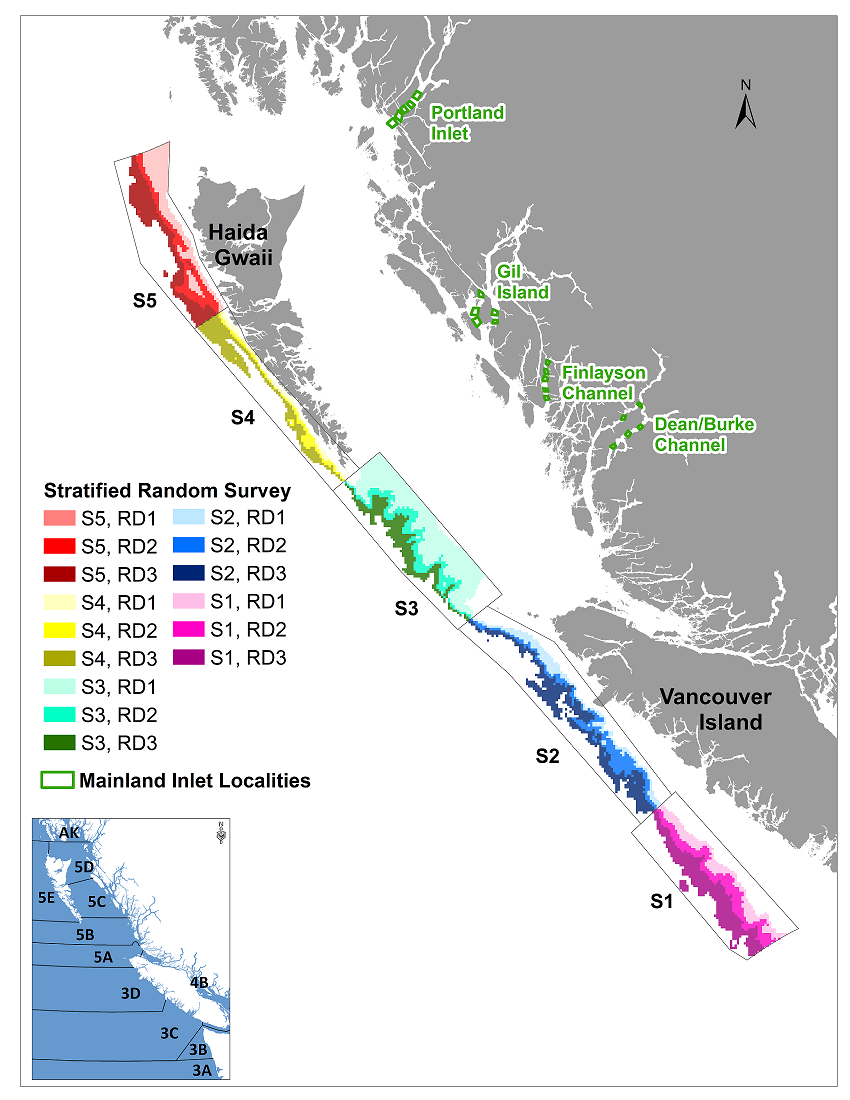
\includegraphics[width=400px,height=500px]{C:/github/surveyreport/figures/Figure_1_Report_Overview_survey_2019}}{Figure \ref{fig:figure1}} 

}

\caption{Location of the boundaries of the mainland inlet localities, and the five spatial areas (S\textsubscript{1}-S\textsubscript{5}) of the stratified random survey design. The three depths strata (RD\textsubscript{1}-RD\textsubscript{3}) are colour-coded, nested within each of the five spatial strata. The insert depicts the commercial groundfish management areas.}\label{fig:figure1}
\end{figure}
\clearpage


\begin{figure}[htb]

{\centering \pdftooltip{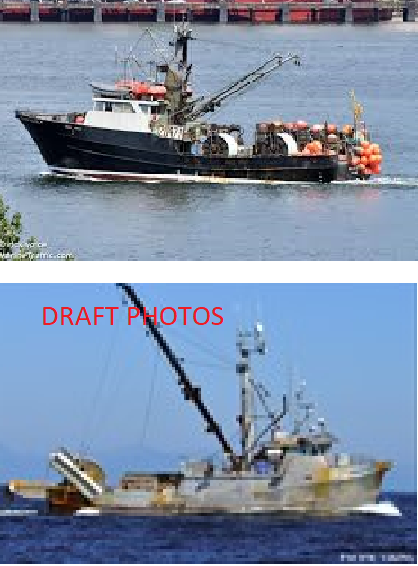
\includegraphics[width=350px,height=600px]{C:/github/surveyreport/figures/Figure_2_vessels}}{Figure \ref{fig:figure2}} 

}

\caption{Image of F/V Ocean Pearl of 35.66 meters (top) and F/V Pacific Viking of 25.34 meters (bottom). Photo credit: Joe Smith.}\label{fig:figure2}
\end{figure}
\clearpage


\begin{figure}[htb]

{\centering \pdftooltip{\includegraphics[width=350px,height=600px]{C:/github/surveyreport/figures/Figure_3_Report_S1_S5_20182019}}{Figure \ref{fig:figure3}} 

}

\caption{Start locations of survey sets (red markers) conducted in 2018 (top) and 2019 (bottom) for the stratified random survey areas S\textsubscript{1} through S\textsubscript{5}.}\label{fig:figure3}
\end{figure}
\clearpage


\begin{figure}[htb]

{\centering \pdftooltip{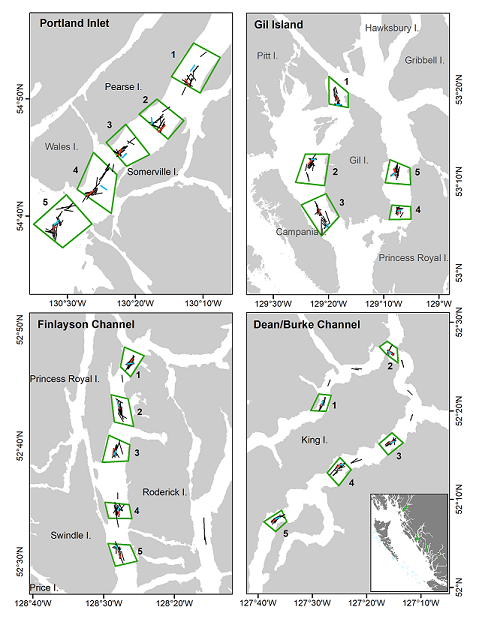
\includegraphics[width=400px]{C:/github/surveyreport/figures/Figure_4_Report_Inlets_2019}}{Figure \ref{fig:figure4}} 

}

\caption{Location of the traditional survey sets within the mainland inlet localities since 1994. The setlines for 2018 are shown in blue and setlines for 2019 are shown in red.}\label{fig:figure4}
\end{figure}
\clearpage


\begin{figure}[htb]

{\centering \pdftooltip{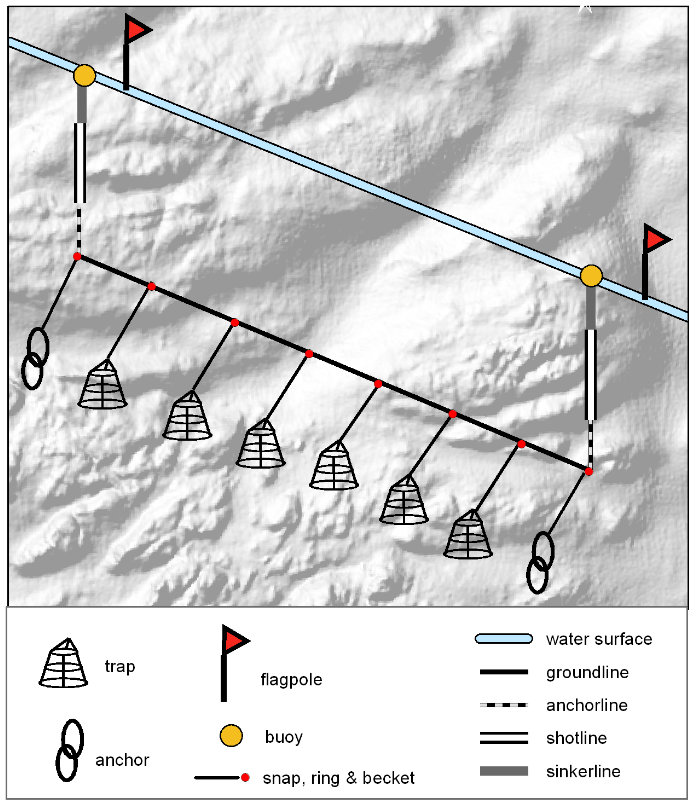
\includegraphics[width=400px]{C:/github/surveyreport/figures/Figure_5_gearelements}}{Figure \ref{fig:figure5}} 

}

\caption{Trap gear elements consisting of 25 baited traps snapped to beckets along a groundline.}\label{fig:figure5}
\end{figure}
\clearpage


\begin{figure}[htb]

{\centering \pdftooltip{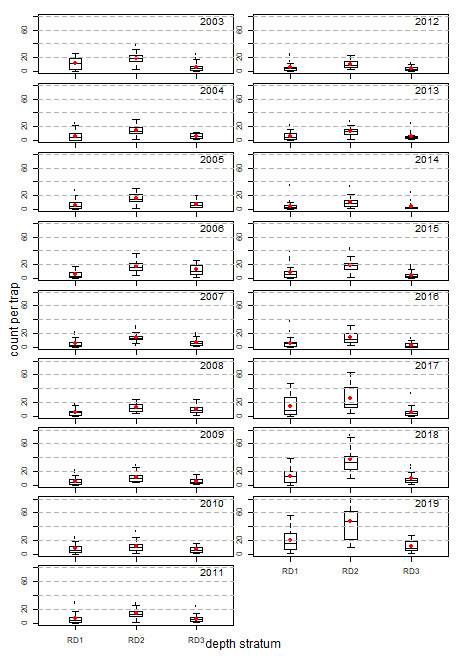
\includegraphics[width=400px,height=620px]{C:/github/surveyreport/figures/Figure_6_cpue}}{Figure \ref{fig:figure6}} 

}

\caption{Distribution of yearly catch rates for Type 3 tagging sets summarised by a boxplot. Each panel shows catch rates grouped by depth strata from shallow to deep (RD\textsubscript{1}-RD\textsubscript{3}) for each year of the StRS survey. The red circles show the mean catch rates for each depth stratum.}\label{fig:figure6}
\end{figure}
\clearpage


\begin{figure}[htb]

{\centering \pdftooltip{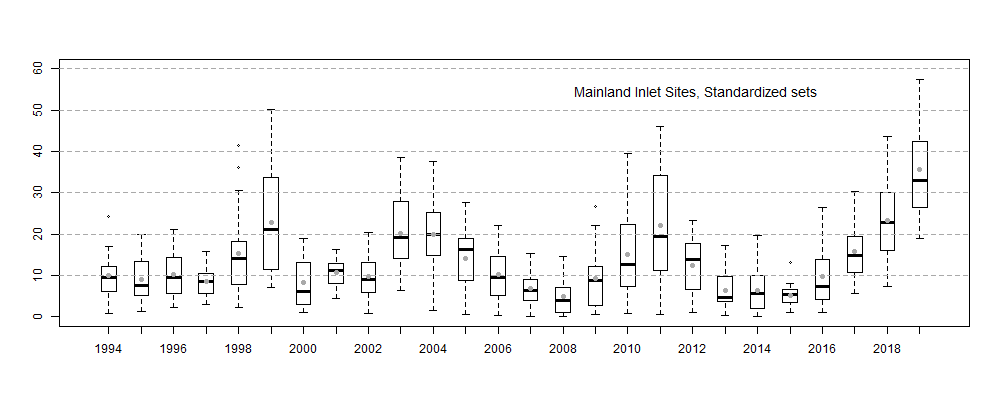
\includegraphics[width=500px,height=300px]{C:/github/surveyreport/figures/Figure_7_InletCPUE}}{Figure \ref{fig:figure7}} 

}

\caption{Distribution of catch rates summarised by boxplots for standardized sets conducted at mainland Inlet localities.}\label{fig:figure7}
\end{figure}
\clearpage


\begin{figure}[htb]

{\centering \pdftooltip{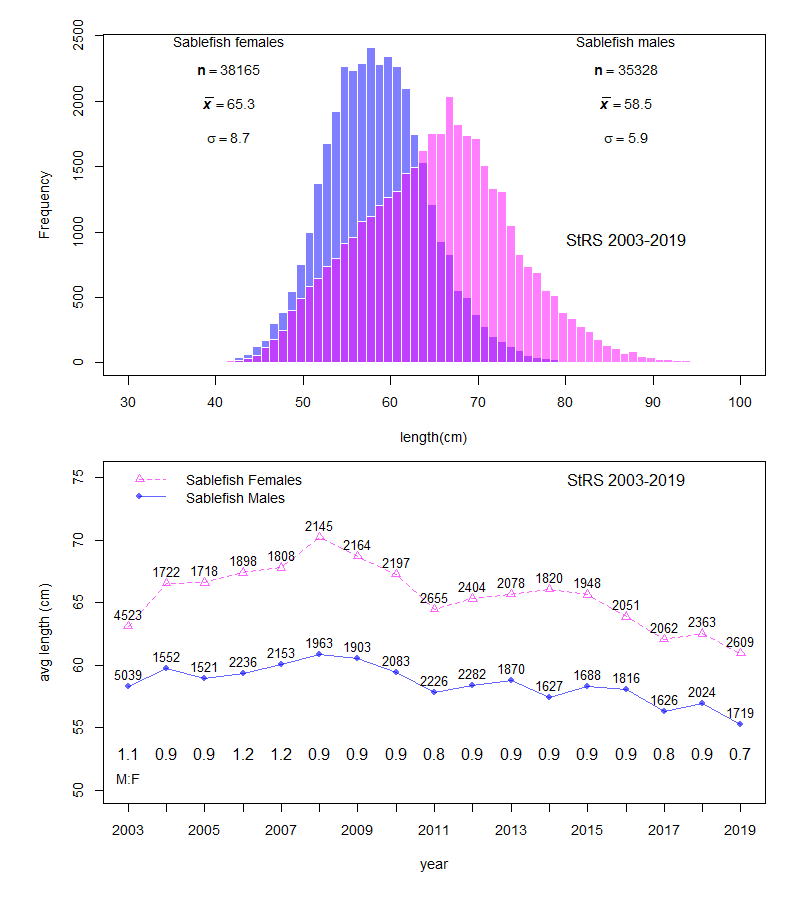
\includegraphics[width=400px,height=500px]{C:/github/surveyreport/figures/Figure_8_lengths}}{Figure \ref{fig:figure8}} 

}

\caption{Top: Length frequencies for male sablefish (blue-violet) and female sablefish (fuchsia) up to 2019 for all StRS sets. The number of specimens is denoted by the letter n, the mean indicated by the xbar \(\overline{x}\) and the standard deviation is represented by the symbol sigma \(\Sigma\). Bottom: Average length and ratios of male and female sablefish by year. Counts by sex are shown across the top of the lines.}\label{fig:figure8}
\end{figure}
\clearpage


\begin{figure}[htb]

{\centering \pdftooltip{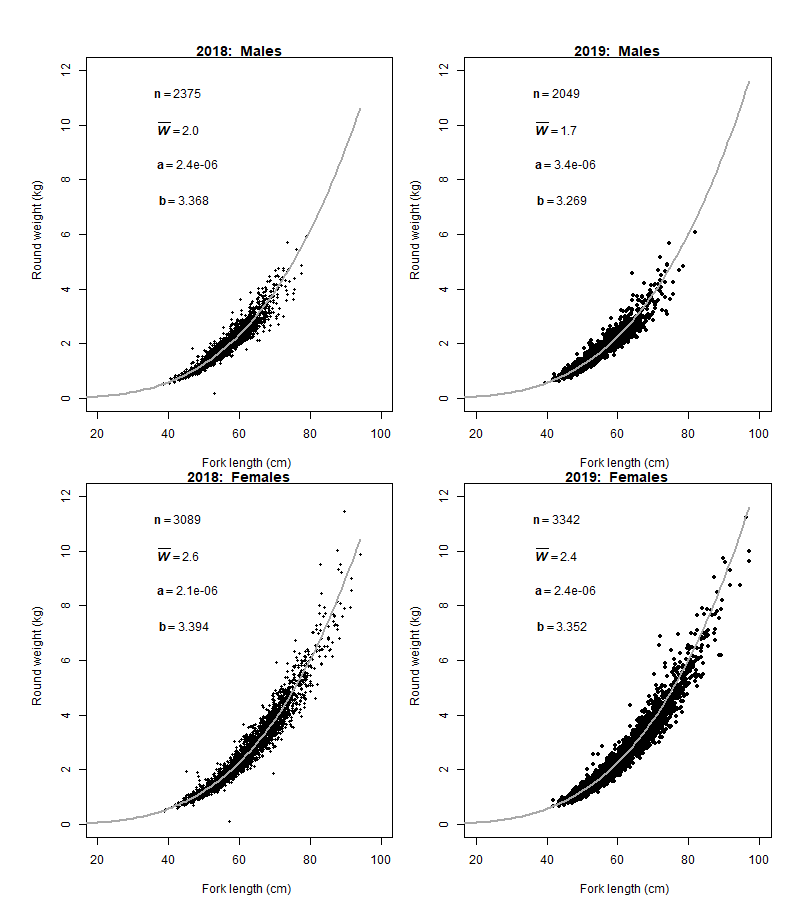
\includegraphics[width=400px,height=500px]{C:/github/surveyreport/figures/Figure_9_Lenwt}}{Figure \ref{fig:figure9}} 

}

\caption{Sablefish fork length (L in cm) vs weight (W in kg) for males and females for the 2018 (left) and 2019 (right) surveys.}\label{fig:figure9}
\end{figure}
\clearpage


\begin{figure}[htb]

{\centering \pdftooltip{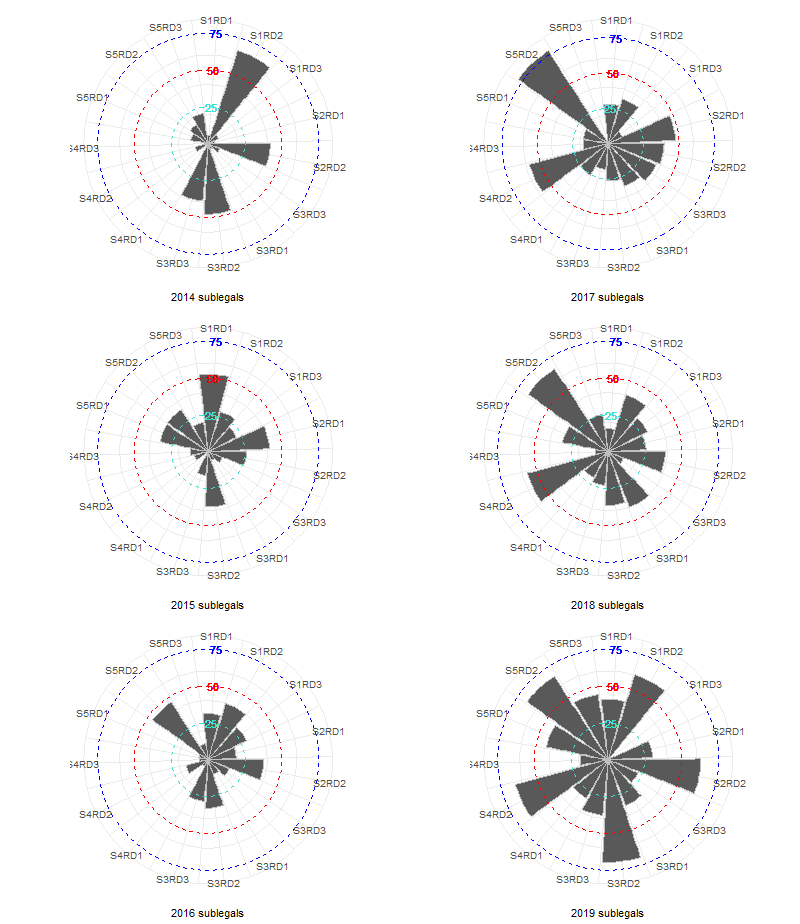
\includegraphics[width=500px,height=600px]{C:/github/surveyreport/figures/Figure_10_polar}}{Figure \ref{fig:figure10}} 

}

\caption{The percentage of sub-legal sablefish (\textless55 cm fork length) sampled in the StRS survey strata and depth strata since the year 2014, denoted by the green (25\%), red (50\%) and blue (75\%) dashed lines.}\label{fig:figure10}
\end{figure}
\clearpage


\begin{figure}[htb]

{\centering \pdftooltip{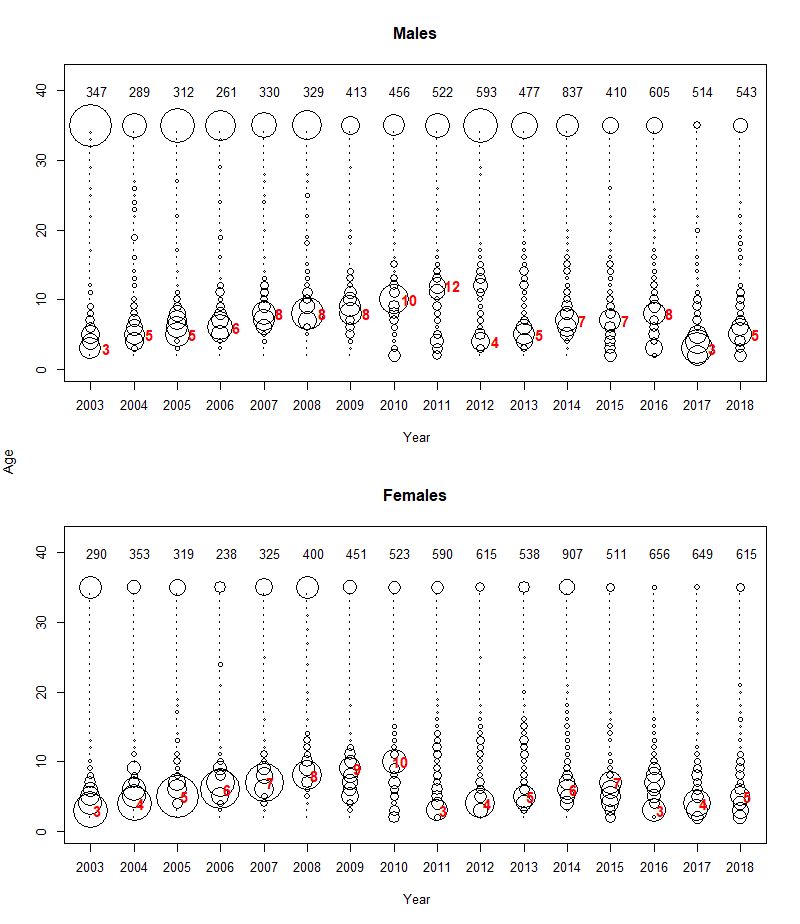
\includegraphics[width=400px,height=500px]{C:/github/surveyreport/figures/Figure_11_ages}}{Figure \ref{fig:figure11}} 

}

\caption{Bubble plot for male and female sablefish ages by survey year from StRS sets that have been aged. The sizes of the circles are proportional to the number of fish with given ages. Fish age 35 and older are included in one bubble. The total number(n) of fish aged are listed across the top of each panel. The ages with the highest ratios are posted to the right of each bubble.}\label{fig:figure11}
\end{figure}
\clearpage


\begin{figure}[htb]

{\centering \pdftooltip{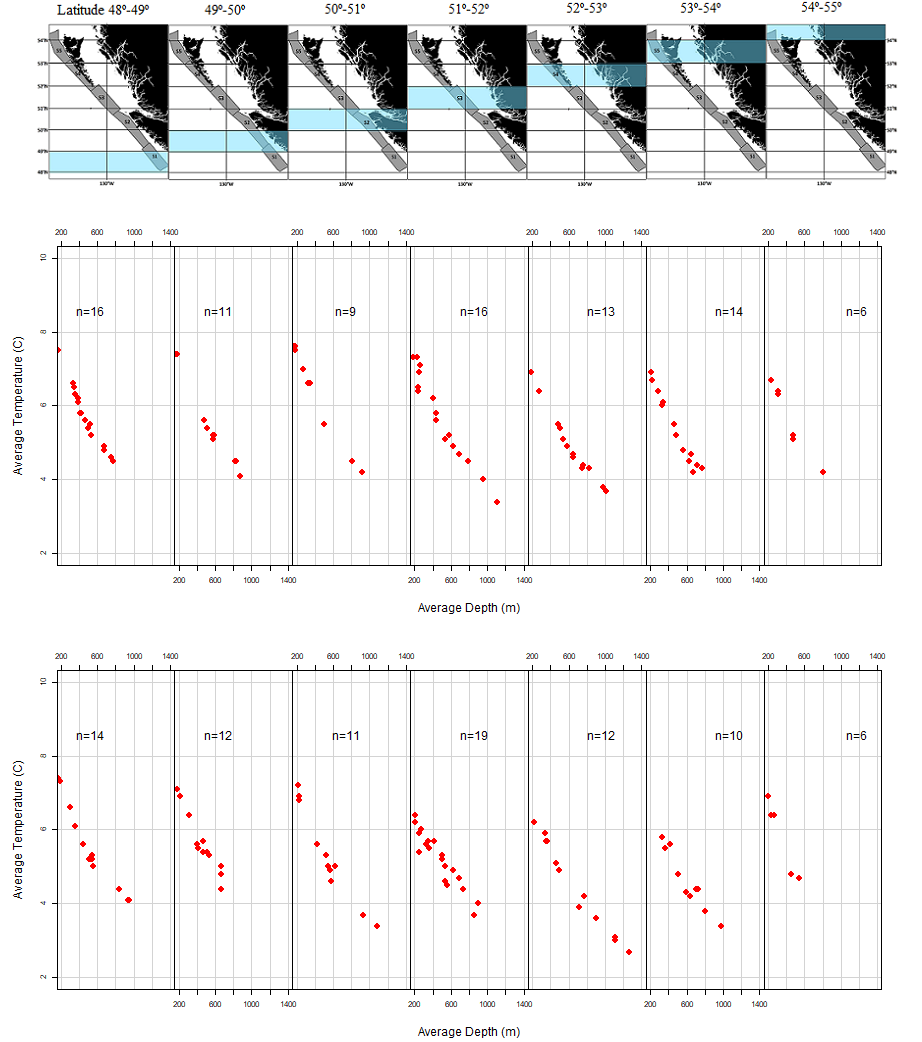
\includegraphics[width=500px,height=600px]{C:/github/surveyreport/figures/Figure_12_coplot}}{Figure \ref{fig:figure12}} 

}

\caption{Coplot of average depth(m) vs average temperature (\(^\circ\)C) for a given 1-degree latitude range (blue bands) for 2018 (top) and 2019 (bottom). The number of fishing sets deployed with a SBE 39 recorder are represented by n.}\label{fig:figure12}
\end{figure}
\clearpage


\begin{figure}[htb]

{\centering \pdftooltip{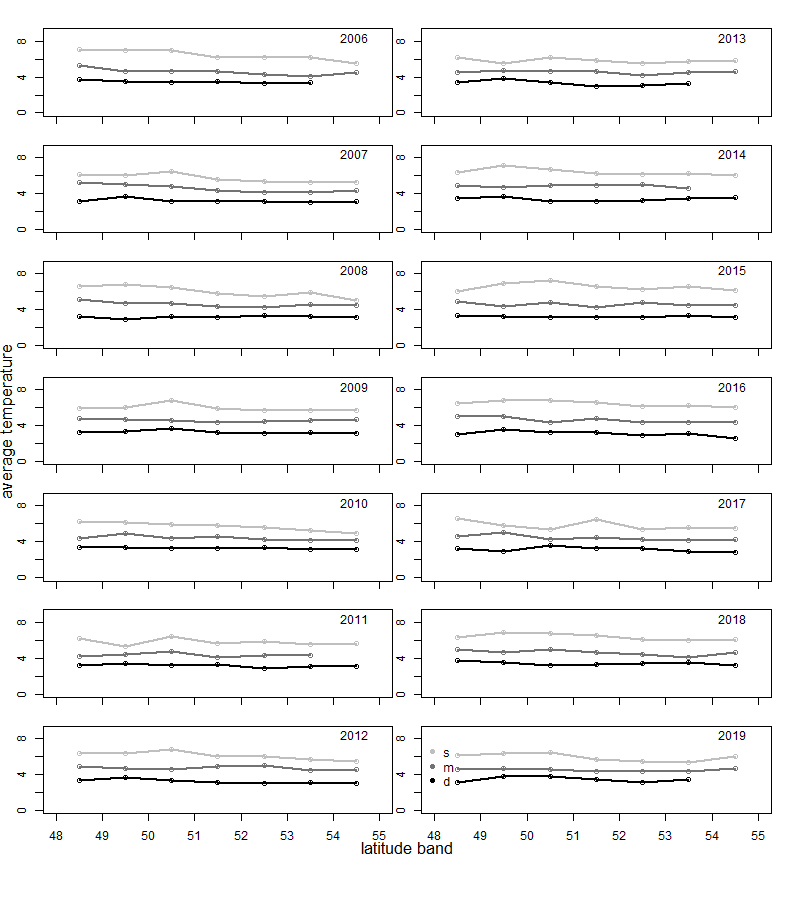
\includegraphics[width=400px,height=580px]{C:/github/surveyreport/figures/Figure_13_seabirdavg}}{Figure \ref{fig:figure13}} 

}

\caption{Average temperatures as reported from the Sea-bird SBE 39 loggers at 1-degree latitude intervals and three depth intervals: s: 100-250 fathoms (183 to 457 meters), m: 250-450 fathoms (458-823 meters) and d: 450-750 fathoms (824-1372 meters).}\label{fig:figure13}
\end{figure}
\clearpage

\begin{appendices}
\counterwithin{figure}{section}
\counterwithin{table}{section}
\counterwithin{equation}{section}

\clearpage

\section{LIST OF TRADITIONAL LOCALITIES.}
\label{app:first-appendix}

List of localities visited in the traditional component of the sablefish research and assessment surveys from 1988 through 2019. Standardized sets (light blue boxes and half boxes) were conducted in offshore indexing localities from 1988 to 2010. Sablefish were tagged and released (dark blue half boxes) from standardized sets at offshore indexing localities beginning in 1991 and ending in 2007. In 1995, offshore tagging localities where only traditional tagging sets (red boxes) occurred were added in 1995 and discontinued in 2008. Mainland Inlet localities where standardized sets (green boxes) were conducted began in 1994 and continued through to 2019. Starting in 2002 (dark green), five standard fishing areas were chosen to ensure the consistency with the positions of sets conducted in previous years.
\begin{center}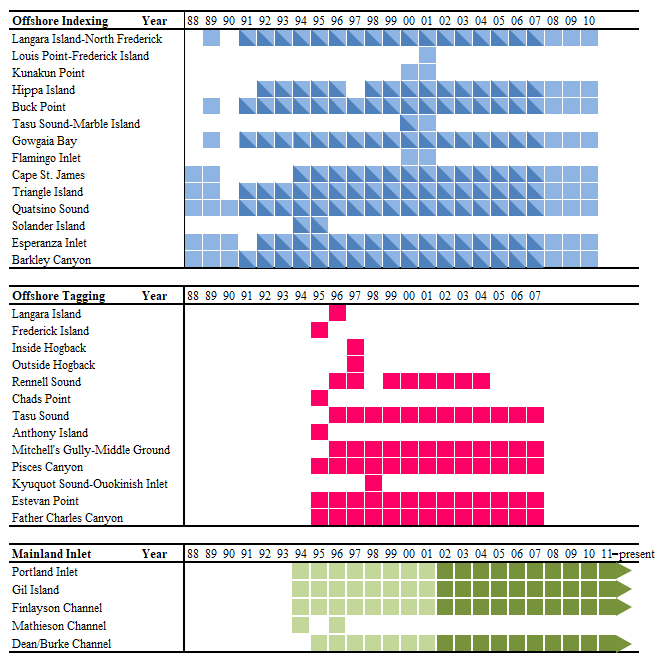
\includegraphics[width=400px,height=400px]{c:/github/surveyreport/figures/AppendixSurveyHistory2} \end{center}
\clearpage

\section{LIST OF SABLEFISH RESEARCH AND ASSESSMENT SURVEYS.}
\label{app:second-appendix}

\begingroup\fontsize{7}{9}\selectfont
\begin{longtable}{rlllrr}
\toprule
\textbf{Year} & \textbf{Dates} & \textbf{Vessel} & \textbf{Captain} & \textbf{Set.Count} & \textbf{GFBIO.Trip}\\
\midrule
1988 & Oct 28  - Nov 24 & VICIOUS FISHER & VANCE FLETCHER & 16 & 43990\\
1989 & Oct 19  - Nov 18 & LA PORSCHE & SIGURD BRYNJOLFSON & 29 & 43910\\
1990 & Nov  8  - Nov 18 & VIKING STAR & DOUG FARRINGTON & 24 & 43750\\
1991 & Oct  9  - Oct 29 & W. E. RICKER & ALAN FARRINGTON & 32 & 43673\\
1992 & Oct 13  - Nov  4 & W. E. RICKER & RON ROBERTS & 38 & 43670\\
1993 & Oct 19  - Nov 11 & W. E. RICKER & ALAN FARRINGTON & 42 & 43650\\
1994 & Oct 13  - Oct 31 & LA PORSCHE & RICHARD BEAUVAIS & 39 & 43630\\
1994 & Oct 18  - Nov 13 & WESTERN VIKING & RICK JONES & 27 & 43390\\
1995 & Oct  8  - Oct 20 & OCEAN PEARL & ROBERT FRAUMENI & 29 & 43270\\
1995 & Oct 11  - Oct 28 & VICTOR F & MICHAEL DERRY & 34 & 43330\\
1995 & Oct  1  - Oct 31 & VIKING SUNRISE & JASON OLSEN & 40 & 43350\\
1996 & Sep 26  - Oct 10 & OCEAN PEARL & MICHAEL DERRY & 32 & 43039\\
1996 & Sep 30  - Oct 22 & VIKING STAR & OTTO ELVAN & 49 & 43210\\
1996 & May 10  - May 30 & VIKING SUNRISE & ALBERT (DEACON) MELNYCHUK & 42 & 43024\\
1997 & Sep 26  - Oct 21 & OCEAN PEARL & MICHAEL DERRY & 74 & 42699\\
1997 & May 20  - Jun 10 & VIKING SUNRISE & ALBERT (DEACON) MELNYCHUK & 42 & 42760\\
1998 & Sep 22  - Oct 17 & OCEAN PEARL & MICHAEL DERRY & 89 & 41122\\
1999 & Sep 29  - Oct 30 & OCEAN PEARL & MICHAEL DERRY & 109 & 40589\\
2000 & Oct  8  - Nov 14 & PACIFIC VIKING & ALBERT (DEACON) MELNYCHUK & 131 & 40517\\
2001 & Oct  6  - Nov  6 & OCEAN PEARL & MICHAEL DERRY & 134 & 43233\\
2002 & Oct  4  - Nov  7 & PACIFIC VIKING & ALBERT (DEACON) MELNYCHUK & 125 & 48120\\
2002 & Oct  5  - Nov 13 & VIKING SUNRISE & JASON OLSEN & 90 & 48110\\
2003 & Oct 15  - Nov 13 & OCEAN PEARL & MICHAEL DERRY & 94 & 52100\\
2003 & Oct  7  - Nov 10 & VIKING STAR & JIM FARRINGTON & 84 & 52120\\
2004 & Oct  5  - Nov 15 & MILBANKE SOUND & DON QUAST & 95 & 58145\\
2004 & Oct  5  - Nov  3 & OCEAN MARAUDER & ALBERT (DEACON) MELNYCHUK & 84 & 57360\\
2005 & Oct  4  - Nov  2 & PACIFIC VIKING & ALBERT (DEACON) MELNYCHUK & 84 & 60529\\
2005 & Oct  7  - Nov 17 & VIKING SUNRISE & RORY JOHNSON & 88 & 60503\\
2006 & Oct  1  - Nov  1 & PACIFIC VIKING & ALBERT (DEACON) MELNYCHUK & 98 & 62966\\
2006 & Oct  2  - Nov 15 & SENA II & TIM JOYS & 98 & 62666\\
2007 & Oct  7  - Nov 12 & PACIFIC VIKING & ALBERT (DEACON) MELNYCHUK & 99 & 65106\\
2007 & Oct  8  - Nov 12 & VIKING TIDE & JASON OLSEN & 91 & 65107\\
2008 & Sep 29  - Nov 16 & OCEAN PEARL & ROBERT FRAUMENI & 157 & 67007\\
2009 & Oct  8  - Nov 25 & OCEAN PEARL & ROBERT FRAUMENI & 155 & 69067\\
2010 & Oct  9  - Nov 30 & OCEAN PEARL & ROBERT FRAUMENI & 153 & 70787\\
2011 & Oct  9  - Nov 21 & OCEAN PEARL & DARCY NICHOLS & 132 & 72067\\
2012 & Oct  9  - Nov 17 & OCEAN PEARL & DARCY NICHOLS & 135 & 73190\\
2013 & Oct 11  - Nov 17 & PACIFIC VIKING & ALBERT (DEACON) MELNYCHUK & 111 & 74872\\
2014 & Oct  9  - Nov 17 & OCEAN PEARL & DARCY NICHOLS & 111 & 76150\\
2015 & Oct  9  - Nov 20 & PACIFIC VIKING & ALBERT (DEACON) MELNYCHUK & 111 & 77830\\
2016 & Oct  7  - Nov 22 & OCEAN PEARL & DARCY NICHOLS & 111 & 80471\\
2017 & Oct  6  - Nov 21 & PACIFIC VIKING & ALBERT (DEACON) MELNYCHUK & 109 & 82790\\
2018 & Oct  9  - Nov 19 & OCEAN PEARL & DARCY NICHOLS & 111 & 84250\\
2019 & Oct  8  - Nov 25 & PACIFIC VIKING & ALBERT (DEACON) MELNYCHUK & 109 & 85230\\
\bottomrule
\end{longtable}
\endgroup{}

\clearpage

\section{SET DETAILS 2018.}
\label{app:third-appendix}

Details of sets completed during the 2018 survey program (F/V Ocean Pearl). Sets are listed by stratum/inlet name, set type, depth stratum, start date, end of gear deployment time and duration in minutes. The depth strata for type 3 tagging sets include RD\textsubscript{1} (100-250 fathoms), RD\textsubscript{2} (250-450 fathoms) and RD\textsubscript{3} (450-750 fathoms). The position data includes the major area along with the start and end latitude and longitude in degrees decimal minutes. The bottom depths (in meters) of the fishing set are shown with the mean bottom depth calculated from recordings at one minute intervals between the start and end of the set. The number of traps fished for each set excludes open traps, while holed or fouled traps have been included. Sets that successfully deployed a Seabird SBE temperature and pressure recorder, a Hobo accelerometer or a Concerto CTD are indicated with an `x'.
\begin{landscape}\begingroup\fontsize{8}{10}\selectfont
\begin{longtable}{>{\raggedright\arraybackslash}p{1.2cm}>{\raggedleft\arraybackslash}p{0.5cm}>{\raggedright\arraybackslash}p{0.4cm}>{\raggedright\arraybackslash}p{0.4cm}>{\raggedright\arraybackslash}p{0.9cm}>{\raggedright\arraybackslash}p{0.7cm}>{\raggedleft\arraybackslash}p{0.7cm}>{\raggedright\arraybackslash}p{0.5cm}>{\raggedright\arraybackslash}p{1.6cm}>{\raggedright\arraybackslash}p{1.6cm}>{\raggedright\arraybackslash}p{1.6cm}>{\raggedright\arraybackslash}p{1.6cm}>{\raggedleft\arraybackslash}p{0.7cm}>{\raggedleft\arraybackslash}p{0.7cm}>{\raggedleft\arraybackslash}p{0.5cm}>{\raggedleft\arraybackslash}p{0.6cm}>{\raggedright\arraybackslash}p{0.4cm}>{\raggedright\arraybackslash}p{0.4cm}>{\raggedright\arraybackslash}p{0.4cm}}
\toprule
Spatial Stratum & Set & Type & Depth Stratum & Date & Time & Duration & Area & Latitude & Longitude & Latitude & Longitude & Start & End & Mean & Traps Fished & SBE 39 & Hobo & CTD\\
\midrule
\endfirsthead
\multicolumn{19}{@{}l}{continued.}\\
\toprule
Spatial Stratum & Set & Type & Depth Stratum & Date & Time & Duration & Area & Latitude & Longitude & Latitude & Longitude & Start & End & Mean & Traps Fished & SBE 39 & Hobo & CTD\\
\midrule
\endhead
\
\endfoot
\bottomrule
\endlastfoot
S1 & 1 & StRS & RD3 & Oct 10 & 12:03 & 1351 & 3C & 48° 0.9'N & 126° 4.9'W & 48° 0.9'N & 126° 4.1'W & 1035 & 1100 & 1056 & 25 & x &  & \\
S1 & 2 & StRS & RD3 & Oct 10 & 14:11 & 1350 & 3C & 48° 4.4'N & 126° 4.7'W & 48° 4.4'N & 126° 5.6'W & 857 & 949 & 890 & 25 & x &  & \\
S1 & 3 & StRS & RD2 & Oct 10 & 16:04 & 1361 & 3C & 48° 5.3'N & 125° 55.4'W & 48° 4.7'N & 125° 55.5'W & 584 & 707 & 639 & 25 & x & x & \\
S1 & 4 & StRS & RD1 & Oct 10 & 18:05 & 1336 & 3C & 48° 7.1'N & 125° 56.6'W & 48° 6.7'N & 125° 57.2'W & 377 & 430 & 404 & 25 & x & x & \\
S1 & 5 & StRS & RD2 & Oct 10 & 20:13 & 1396 & 3C & 48° 7.7'N & 126° 11.2'W & 48° 8.1'N & 126° 11.7'W & 466 & 458 & 467 & 25 & x & x & \\
S1 & 6 & StRS & RD1 & Oct 12 & 07:59 & 1325 & 3C & 48° 2.1'N & 126° 7.6'W & 48° 1.9'N & 126° 8.4'W & 185 & 189 & 187 & 25 & x & x & \\
S1 & 7 & StRS & RD3 & Oct 12 & 10:03 & 1434 & 3C & 48° 3.4'N & 126° 19.5'W & 48° 3.5'N & 126° 18.5'W & 1077 & 820 & 899 & 25 & x & x & \\
S1 & 8 & StRS & RD2 & Oct 12 & 12:02 & 1433 & 3C & 48° 8.8'N & 126° 17.7'W & 48° 8.6'N & 126° 17'W & 530 & 466 & 476 & 25 & x & x & \\
S1 & 9 & StRS & RD2 & Oct 12 & 14:13 & 1436 & 3C & 48° 4.1'N & 126° 22.5'W & 48° 3.4'N & 126° 22.5'W & 553 & 725 & 635 & 25 & x & x & \\
S1 & 10 & StRS & RD2 & Oct 12 & 16:02 & 1448 & 3C & 48° 4.4'N & 126° 28.9'W & 48° 4.3'N & 126° 28.1'W & 474 & 539 & 500 & 25 & x & x & \\
S1 & 11 & StRS & RD3 & Oct 12 & 18:23 & 1502 & 3C & 48° 6.8'N & 126° 39.2'W & 48° 6.7'N & 126° 38.3'W & 1337 & 1338 & 1339 & 25 & x & x & \\
S1 & 12 & StRS & RD2 & Oct 14 & 08:01 & 1335 & 3C & 48° 3.1'N & 126° 29'W & 48° 2.5'N & 126° 29.1'W & 565 & 603 & 589 & 25 & x & x & \\
S1 & 13 & StRS & RD2 & Oct 14 & 10:02 & 1349 & 3C & 48° 4.5'N & 126° 30.8'W & 48° 4.4'N & 126° 31.6'W & 461 & 497 & 481 & 25 & x & x & \\
S1 & 14 & StRS & RD3 & Oct 14 & 12:02 & 1377 & 3C & 48° 4.4'N & 126° 35.7'W & 48° 4.4'N & 126° 36.6'W & 866 & 924 & 859 & 25 & x & x & \\
S1 & 15 & StRS & RD1 & Oct 14 & 14:03 & 1389 & 3C & 48° 0.8'N & 126° 35.5'W & 48° 0.8'N & 126° 36.3'W & 382 & 434 & 408 & 25 & x & x & \\
S1 & 16 & StRS & RD1 & Oct 14 & 16:00 & 1396 & 3C & 48° 1.9'N & 126° 33.4'W & 48° 1.7'N & 126° 32.5'W & 442 & 256 & 375 & 25 & x & x & \\
S1 & 17 & StRS & RD2 & Oct 14 & 18:03 & 1404 & 3C & 48° 5.3'N & 126° 38.3'W & 48° 5.3'N & 126° 37.4'W & 533 & 659 & 589 & 25 & x & x & x\\
S1 & 18 & StRS & RD1 & Oct 14 & 20:04 & 1381 & 3C & 48° 7.5'N & 126° 33.2'W & 48° 7.4'N & 126° 32.3'W & 430 & 207 & 322 & 25 & x & x & \\
S1 & 19 & StRS & RD1 & Oct 16 & 08:04 & 1328 & 3D & 49° 7.4'N & 127° 6.9'W & 49° 7.7'N & 127° 6.1'W & 206 & 193 & 199 & 25 & x & x & \\
S2 & 20 & StRS & RD2 & Oct 16 & 09:54 & 1355 & 3D & 49° 0.3'N & 127° 15.1'W & 49° 0.7'N & 127° 15.4'W & 643 & 627 & 608 & 25 & x & x & \\
S2 & 21 & StRS & RD1 & Oct 16 & 11:56 & 1358 & 3D & 49° 2.9'N & 127° 13.3'W & 49° 3.5'N & 127° 13.3'W & 209 & 200 & 205 & 25 & x & x & \\
S2 & 22 & StRS & RD3 & Oct 16 & 14:09 & 1398 & 3D & 49° 0.6'N & 127° 26.3'W & 49° 0.6'N & 127° 25.5'W & 921 & 948 & 925 & 25 & x & x & \\
S2 & 23 & StRS & RD2 & Oct 16 & 16:00 & 1412 & 3D & 49° 3.9'N & 127° 32.2'W & 49° 3.7'N & 127° 32.8'W & 637 & 711 & 655 & 25 & x & x & \\
S2 & 24 & StRS & RD2 & Oct 16 & 18:04 & 1413 & 3D & 49° 0.3'N & 127° 31.1'W & 49° 9.8'N & 127° 31.1'W & 685 & 637 & 651 & 25 & x & x & x\\
S2 & 25 & StRS & RD2 & Oct 16 & 19:32 & 1426 & 3D & 49° 0.3'N & 127° 27.8'W & 49° 0.3'N & 127° 28.7'W & 552 & 579 & 559 & 25 & x & x & \\
S2 & 26 & StRS & RD2 & Oct 18 & 08:08 & 1332 & 3D & 49° 0.4'N & 127° 54.1'W & 49° 1'N & 127° 54.1'W & 718 & 751 & 739 & 25 & x & x & \\
S2 & 27 & StRS & RD3 & Oct 18 & 10:08 & 1352 & 3D & 49° 3.5'N & 128° 0.7'W & 49° 2.9'N & 128° 0.7'W & 1120 & 1032 & 1046 & 25 & x & x & \\
S2 & 28 & StRS & RD2 & Oct 18 & 12:12 & 1367 & 3D & 49° 9'N & 127° 51.4'W & 49° 9.4'N & 127° 52'W & 738 & 736 & 660 & 25 & x & x & \\
S2 & 29 & StRS & RD1 & Oct 18 & 14:04 & 1396 & 3D & 50° 0.3'N & 127° 54.7'W & 50° 0.7'N & 127° 55.5'W & 194 & 406 & 334 & 25 & x & x & x\\
S2 & 30 & StRS & RD3 & Oct 18 & 16:14 & 1404 & 3D & 50° 0.7'N & 128° 3.9'W & 50° 0.4'N & 128° 3.9'W & 1174 & 1143 & 1167 & 25 & x & x & \\
S2 & 31 & StRS & RD3 & Oct 18 & 18:11 & 1428 & 3D & 49° 9.1'N & 128° 2.9'W & 49° 9.1'N & 128° 3.9'W & 1041 & 994 & 1035 & 25 & x & x & \\
S2 & 32 & StRS & RD3 & Oct 20 & 08:11 & 1415 & 3D & 50° 7.8'N & 128° 28.9'W & 50° 8.4'N & 128° 28.9'W & 1027 & 1029 & 1011 & 25 & x & x & \\
S2 & 33 & StRS & RD1 & Oct 20 & 10:01 & 1413 & 3D & 50° 3'N & 128° 22.1'W & 50° 3.6'N & 128° 22.1'W & 208 & 202 & 205 & 25 & x & x & \\
S2 & 34 & StRS & RD1 & Oct 20 & 11:37 & 1402 & 3D & 50° 6.3'N & 128° 25.4'W & 50° 6.9'N & 128° 25.4'W & 195 & 194 & 194 & 24 & x & x & \\
S2 & 35 & StRS & RD1 & Oct 20 & 15:35 & 1430 & 5A & 50° 2.9'N & 129° 2.5'W & 50° 2.5'N & 129° 2.2'W & 221 & 301 & 318 & 25 & x & x & x\\
S2 & 36 & StRS & RD2 & Oct 20 & 17:04 & 1449 & 5A & 50° 2.4'N & 129° 4.4'W & 50° 2.4'N & 129° 5.3'W & 555 & 609 & 533 & 25 & x & x & \\
S2 & 37 & StRS & RD1 & Oct 20 & 19:02 & 1440 & 5A & 50° 4'N & 129° 14.4'W & 50° 3.6'N & 129° 14.2'W & 278 & 304 & 347 & 25 & x & x & \\
Dean/Burke & 38 & Inlet &  & Oct 23 & 12:07 & 1078 & 5B & 52° 0.7'N & 127° 36.8'W & 52° 0'N & 127° 35.9'W & 438 & 440 & 441 & 25 & x & x & \\
Dean/Burke & 39 & Inlet &  & Oct 23 & 13:58 & 1130 & 5B & 52° 3.8'N & 127° 25'W & 52° 4'N & 127° 24.2'W & 594 & 596 & 595 & 25 & x & x & \\
Dean/Burke & 40 & Inlet &  & Oct 23 & 16:09 & 1107 & 5B & 52° 6.3'N & 127° 15.6'W & 52° 6.6'N & 127° 14.8'W & 578 & 578 & 579 & 25 & x & x & x\\
Dean/Burke & 41 & Inlet &  & Oct 23 & 18:11 & 1132 & 5B & 52° 6.4'N & 127° 15.4'W & 52° 6.7'N & 127° 16'W & 515 & 537 & 527 & 25 & x & x & \\
Dean/Burke & 42 & Inlet &  & Oct 23 & 19:56 & 1187 & 5B & 52° 1.2'N & 127° 28.1'W & 52° 0.6'N & 127° 28.3'W & 505 & 516 & 513 & 25 & x & x & \\
Finlayson & 43 & Inlet &  & Oct 25 & 11:57 & 1093 & 5C & 52° 7.1'N & 128° 25.9'W & 52° 7'N & 128° 26.7'W & 572 & 576 & 576 & 25 & x & x & \\
Finlayson & 44 & Inlet &  & Oct 25 & 14:04 & 1098 & 5C & 52° 4'N & 128° 28.1'W & 52° 3.4'N & 128° 27.9'W & 710 & 634 & 665 & 25 & x & x & x\\
Finlayson & 45 & Inlet &  & Oct 25 & 16:07 & 1107 & 5C & 52° 9.6'N & 128° 28.2'W & 52° 9.2'N & 128° 28.6'W & 644 & 591 & 627 & 25 & x & x & \\
Finlayson & 46 & Inlet &  & Oct 25 & 17:58 & 1117 & 5C & 52° 4.8'N & 128° 27.7'W & 52° 4.3'N & 128° 28'W & 754 & 643 & 677 & 25 & x & x & \\
Finlayson & 47 & Inlet &  & Oct 25 & 20:05 & 1115 & 5C & 52° 1.4'N & 128° 28.2'W & 52° 0.9'N & 128° 27.9'W & 691 & 770 & 729 & 25 & x & x & \\
Gil Island & 48 & Inlet &  & Oct 27 & 12:58 & 1054 & 5C & 53° 8.4'N & 129° 17.7'W & 53° 8.3'N & 129° 18.7'W & 540 & 522 & 539 & 25 & x & x & \\
Gil Island & 49 & Inlet &  & Oct 27 & 14:23 & 1092 & 5C & 53° 2.4'N & 129° 22.3'W & 53° 2.4'N & 129° 23.2'W & 529 & 519 & 548 & 24 & x & x & x\\
Gil Island & 50 & Inlet &  & Oct 27 & 15:55 & 1125 & 5C & 53° 0.4'N & 129° 19.9'W & 53° 0'N & 129° 20.6'W & 683 & 683 & 687 & 25 & x & x & \\
Gil Island & 51 & Inlet &  & Oct 27 & 18:17 & 1141 & 5C & 53° 0.6'N & 129° 8.6'W & 53° 0.9'N & 129° 7.9'W & 552 & 569 & 562 & 25 & x & x & \\
Gil Island & 52 & Inlet &  & Oct 27 & 20:02 & 1166 & 5C & 53° 0.8'N & 129° 7.6'W & 53° 0'N & 129° 6.7'W & 567 & 533 & 545 & 25 & x & x & \\
S3 & 53 & StRS & RD1 & Oct 29 & 08:08 & 1322 & 5B & 51° 2.2'N & 130° 27.6'W & 51° 2.7'N & 130° 26.9'W & 285 & 270 & 275 & 25 & x & x & \\
S3 & 54 & StRS & RD3 & Oct 29 & 11:03 & 1353 & 5B & 51° 0.2'N & 130° 35.6'W & 51° 0.6'N & 130° 35.1'W & 1074 & 1077 & 1079 & 25 & x & x & \\
S3 & 55 & StRS & RD3 & Oct 29 & 12:42 & 1421 & 5B & 51° 5.9'N & 130° 33.8'W & 51° 6.3'N & 130° 33.2'W & 1339 & 1313 & 1321 & 25 & x & x & \\
S3 & 56 & StRS & RD1 & Oct 29 & 14:56 & 1453 & 5B & 51° 4.3'N & 130° 47.5'W & 51° 4.7'N & 130° 48.2'W & 270 & 265 & 267 & 25 & x & x & \\
S3 & 57 & StRS & RD2 & Oct 29 & 16:57 & 1447 & 5B & 51° 6.1'N & 130° 52.4'W & 51° 5.7'N & 130° 53'W & 473 & 723 & 648 & 25 & x & x & \\
S3 & 58 & StRS & RD2 & Oct 29 & 19:00 & 1475 & 5B & 51° 6.7'N & 130° 41.5'W & 51° 7.2'N & 130° 41.6'W & 562 & 506 & 535 & 24 & x & x & \\
S3 & 59 & StRS & RD3 & Oct 31 & 08:24 & 1475 & 5B & 51° 0.4'N & 130° 29.3'W & 51° 0'N & 130° 29.9'W & 1250 & 1322 & 1278 & 25 & x & x & \\
S3 & 60 & StRS & RD2 & Oct 31 & 11:13 & 1462 & 5B & 51° 8.8'N & 130° 16.7'W & 51° 8.3'N & 130° 16.2'W & 460 & 560 & 518 & 25 & x & x & x\\
S3 & 61 & StRS & RD2 & Oct 31 & 12:47 & 1505 & 5B & 51° 4.2'N & 130° 7.5'W & 51° 4'N & 130° 6.8'W & 678 & 636 & 660 & 25 & x & x & \\
S3 & 62 & StRS & RD2 & Oct 31 & 15:29 & 1550 & 5B & 51° 9.8'N & 130° 8.3'W & 51° 9.4'N & 130° 8.2'W & 770 & 767 & 801 & 25 & x & x & \\
S3 & 63 & StRS & RD3 & Oct 31 & 17:37 & 1573 & 5B & 51° 5.4'N & 130° 6.4'W & 51° 4.9'N & 130° 6.5'W & 882 & 865 & 891 & 25 & x & x & \\
S3 & 64 & StRS & RD3 & Oct 31 & 19:44 & 1597 & 5A & 51° 0'N & 130° 8.1'W & 51° 0.6'N & 130° 8.3'W & 892 & 969 & 928 & 25 & x & x & \\
S3 & 65 & StRS & RD1 & Nov  2 & 08:04 & 1354 & 5A & 50° 7.4'N & 129° 24.2'W & 50° 7'N & 129° 23.7'W & 192 & 189 & 190 & 25 & x & x & \\
S3 & 66 & StRS & RD1 & Nov  2 & 10:08 & 1357 & 5A & 51° 0.5'N & 129° 18.7'W & 51° 0'N & 129° 19'W & 247 & 260 & 254 & 25 & x & x & \\
S3 & 67 & StRS & RD1 & Nov  2 & 12:01 & 1352 & 5A & 51° 0.2'N & 129° 26.4'W & 51° 0.9'N & 129° 25.5'W & 286 & 283 & 284 & 25 & x & x & x\\
S3 & 68 & StRS & RD2 & Nov  2 & 14:22 & 1365 & 5A & 51° 0.7'N & 129° 41.1'W & 51° 0.9'N & 129° 41.8'W & 476 & 451 & 466 & 25 & x & x & \\
S3 & 69 & StRS & RD1 & Nov  2 & 16:19 & 1383 & 5A & 51° 3.9'N & 129° 34.7'W & 51° 4.5'N & 129° 34.5'W & 282 & 280 & 283 & 24 & x & x & \\
S3 & 70 & StRS & RD1 & Nov  2 & 18:06 & 1385 & 5B & 51° 9.7'N & 129° 37.3'W & 51° 9.1'N & 129° 37.1'W & 192 & 212 & 199 & 24 & x & x & \\
S3 & 71 & StRS & RD1 & Nov  2 & 20:06 & 1369 & 5B & 51° 1.7'N & 129° 39.7'W & 51° 2.2'N & 129° 39'W & 194 & 184 & 188 & 25 & x & x & \\
S4 & 72 & StRS & RD1 & Nov  4 & 07:10 & 1325 & 5B & 51° 6.4'N & 131° 7.4'W & 51° 5.9'N & 131° 6.7'W & 370 & 258 & 338 & 24 & x & x & \\
S4 & 73 & StRS & RD1 & Nov  4 & 10:01 & 1354 & 5E & 52° 0.3'N & 131° 21'W & 52° 0.7'N & 131° 20.9'W & 217 & 208 & 206 & 24 & x & x & \\
S4 & 74 & StRS & RD2 & Nov  4 & 12:02 & 1361 & 5E & 52° 0.4'N & 131° 22'W & 52° 0.7'N & 131° 21.2'W & 700 & 486 & 563 & 25 & x & x & \\
S4 & 75 & StRS & RD3 & Nov  4 & 14:07 & 1417 & 5E & 52° 0.4'N & 131° 27.6'W & 52° 0.2'N & 131° 26.6'W & 843 & 851 & 841 & 25 & x & x & x\\
S4 & 76 & StRS & RD2 & Nov  4 & 16:00 & 1507 & 5E & 52° 0'N & 131° 31.4'W & 52° 0.1'N & 131° 30.3'W & 513 & 740 & 604 & 25 & x & x & \\
S4 & 77 & StRS & RD2 & Nov  4 & 18:07 & 1501 & 5E & 52° 0.1'N & 131° 29.9'W & 52° 0.6'N & 131° 29'W & 674 & 791 & 717 & 25 & x & x & \\
S4 & 78 & StRS & RD2 & Nov  4 & 20:09 & 1509 & 5E & 52° 1'N & 131° 28.4'W & 52° 1.4'N & 131° 28.9'W & 804 & 804 & 813 & 24 & x & x & \\
S4 & 79 & StRS & RD1 & Nov  4 & 22:02 & 1567 & 5E & 52° 7.8'N & 131° 33.7'W & 52° 7.2'N & 131° 33'W & 202 & 185 & 199 & 25 & x & x & \\
S4 & 80 & StRS & RD1 & Nov  7 & 08:05 & 1331 & 5E & 52° 5.6'N & 131° 58.2'W & 52° 5.3'N & 131° 59'W & 217 & 502 & 307 & 25 & x & x & \\
S4 & 81 & StRS & RD3 & Nov  7 & 10:01 & 1354 & 5E & 52° 6.3'N & 132° 2.2'W & 52° 6.6'N & 132° 3.1'W & 866 & 977 & 935 & 25 & x & x & \\
S4 & 82 & StRS & RD2 & Nov  7 & 12:00 & 1336 & 5E & 52° 8.7'N & 132° 4.1'W & 52° 8.5'N & 132° 5.2'W & 519 & 676 & 589 & 25 & x & x & \\
S4 & 83 & StRS & RD2 & Nov  7 & 14:01 & 1344 & 5E & 52° 3.4'N & 132° 9.7'W & 52° 3.8'N & 132° 10.5'W & 439 & 659 & 544 & 26 &  & x & x\\
S4 & 84 & StRS & RD3 & Nov  7 & 16:46 & 1403 & 5E & 52° 7'N & 132° 36.4'W & 52° 7.5'N & 132° 36.3'W & 1327 & 1300 & 1327 & 25 & x & x & \\
S4 & 85 & StRS & RD3 & Nov  7 & 18:53 & 1453 & 5E & 52° 6.1'N & 132° 46.2'W & 52° 6.7'N & 132° 46.4'W & 1093 & 1168 & 1126 & 25 & x & x & \\
S4 & 86 & StRS & RD3 & Nov  9 & 08:04 & 1338 & 5E & 52° 7.1'N & 132° 40.2'W & 52° 6.5'N & 132° 40'W & 1333 & 1325 & 1337 & 25 & x & x & \\
S4 & 87 & StRS & RD1 & Nov  9 & 09:59 & 1334 & 5E & 53° 0.9'N & 132° 33.7'W & 53° 0.6'N & 132° 33.2'W & 220 & 214 & 222 & 24 & x & x & \\
S4 & 88 & StRS & RD1 & Nov  9 & 12:06 & 1321 & 5E & 53° 0.7'N & 132° 38.5'W & 53° 0.7'N & 132° 39.5'W & 270 & 441 & 359 & 25 & x & x & \\
S5 & 89 & StRS & RD2 & Nov  9 & 14:34 & 1339 & 5E & 53° 1.7'N & 132° 54.8'W & 53° 1.1'N & 132° 54.9'W & 771 & 758 & 775 & 25 & x & x & \\
S5 & 90 & StRS & RD2 & Nov  9 & 16:32 & 1356 & 5E & 53° 4.3'N & 133° 7.2'W & 53° 4.2'N & 133° 6.2'W & 734 & 741 & 737 & 25 &  & x & x\\
S5 & 91 & StRS & RD3 & Nov  9 & 18:33 & 1379 & 5E & 53° 1.8'N & 133° 13.2'W & 53° 1.5'N & 133° 12.4'W & 1049 & 974 & 1029 & 25 & x & x & \\
S5 & 92 & StRS & RD2 & Nov  9 & 20:32 & 1432 & 5E & 53° 5.7'N & 132° 54'W & 53° 5.4'N & 132° 53.1'W & 706 & 695 & 701 & 25 & x & x & \\
S5 & 93 & StRS & RD1 & Nov 11 & 08:03 & 1339 & 5E & 53° 8.9'N & 133° 5'W & 53° 9.4'N & 133° 5.1'W & 360 & 327 & 341 & 25 & x & x & \\
S5 & 94 & StRS & RD2 & Nov 11 & 10:01 & 1354 & 5E & 53° 9.9'N & 133° 11.3'W & 53° 0.5'N & 133° 11.4'W & 541 & 602 & 576 & 25 & x & x & \\
S5 & 95 & StRS & RD1 & Nov 11 & 12:02 & 1348 & 5E & 53° 1'N & 133° 5.3'W & 53° 1.7'N & 133° 5.3'W & 243 & 201 & 221 & 25 &  & x & x\\
S5 & 96 & StRS & RD1 & Nov 11 & 14:00 & 1330 & 5E & 53° 5.2'N & 133° 9.3'W & 53° 5.8'N & 133° 9.1'W & 440 & 431 & 415 & 25 & x & x & \\
S5 & 97 & StRS & RD3 & Nov 11 & 16:03 & 1390 & 5E & 53° 3.6'N & 133° 23.4'W & 53° 4'N & 133° 24.1'W & 819 & 856 & 837 & 24 & x & x & \\
S5 & 98 & StRS & RD3 & Nov 11 & 18:39 & 1448 & 5E & 53° 8.1'N & 133° 45.5'W & 53° 8.6'N & 133° 45.9'W & 950 & 933 & 921 & 25 & x & x & \\
Portland & 99 & Inlet &  & Nov 13 & 14:55 & 1023 & 5D & 54° 9.2'N & 130° 32'W & 54° 9.6'N & 130° 31.3'W & 640 & 640 & 644 & 25 & x & x & \\
Portland & 100 & Inlet &  & Nov 13 & 16:34 & 1075 & 5D & 54° 7.8'N & 130° 17.5'W & 54° 8.4'N & 130° 17.6'W & 484 & 466 & 473 & 25 & x & x & \\
Portland & 101 & Inlet &  & Nov 13 & 18:01 & 1104 & 5D & 54° 2.9'N & 130° 11.3'W & 54° 2.4'N & 130° 11.9'W & 424 & 428 & 427 & 25 & x & x & \\
Portland & 102 & Inlet &  & Nov 13 & 19:34 & 1126 & 5D & 54° 5.3'N & 130° 21.3'W & 54° 5'N & 130° 21.9'W & 501 & 418 & 451 & 24 & x & x & x\\
Portland & 103 & Inlet &  & Nov 13 & 21:00 & 1126 & 5D & 54° 2.6'N & 130° 25.1'W & 54° 2.2'N & 130° 24.2'W & 507 & 478 & 490 & 25 & x & x & \\
S5 & 104 & StRS & RD1 & Nov 15 & 08:41 & 1331 & 5E & 54° 0.8'N & 133° 35.1'W & 54° 0.4'N & 133° 35.9'W & 364 & 359 & 362 & 24 & x & x & \\
S5 & 105 & StRS & RD2 & Nov 15 & 10:01 & 1353 & 5E & 53° 8.9'N & 133° 38.3'W & 53° 9.3'N & 133° 39.1'W & 607 & 575 & 585 & 25 & x & x & \\
S5 & 106 & StRS & RD3 & Nov 15 & 12:03 & 1333 & 5E & 53° 6.2'N & 133° 38.8'W & 53° 5.8'N & 133° 38.3'W & 846 & 842 & 844 & 25 & x & x & \\
S5 & 107 & StRS & RD3 & Nov 15 & 14:04 & 1389 & 5E & 54° 0'N & 133° 46.9'W & 54° 0.6'N & 133° 47.3'W & 1096 & 1081 & 1087 & 25 & x & x & \\
S5 & 108 & StRS & RD2 & Nov 15 & 15:55 & 1398 & 5E & 54° 0.8'N & 133° 47.6'W & 54° 0.1'N & 133° 46.8'W & 549 & 505 & 517 & 25 &  & x & x\\
S5 & 109 & StRS & RD2 & Nov 15 & 18:06 & 1413 & 5E & 54° 5.9'N & 133° 51.6'W & 54° 5.8'N & 133° 50.6'W & 584 & 511 & 548 & 25 & x & x & \\
S5 & 110 & StRS & RD1 & Nov 15 & 19:54 & 1434 & 5E & 54° 8.2'N & 133° 42.6'W & 54° 8.3'N & 133° 41.5'W & 250 & 256 & 254 & 25 & x & x & \\
S5 & 111 & StRS & RD1 & Nov 15 & 21:57 & 1462 & 5E & 54° 0.1'N & 133° 35'W & 54° 0.6'N & 133° 34.7'W & 363 & 365 & 362 & 25 & x & x & \\*
\end{longtable}
\endgroup{}
\end{landscape}
\clearpage

\section{SET DETAILS 2019.}
\label{app:forth-appendix}

Details of sets completed during the 2019 survey program (F/V Pacific Viking). Sets are listed by stratum/inlet name, set type, depth stratum, start date, end of gear deployment time and duration in minutes. The depth strata for type 3 tagging sets include RD\textsubscript{1} (100-250 fathoms), RD\textsubscript{2} (250-450 fathoms) and RD\textsubscript{3} (450-750 fathoms). The position data includes the major area along with the start and end latitude and longitude in degrees decimal minutes. The bottom depths (in meters) of the fishing set are shown with the mean bottom depth calculated from recordings at one minute intervals between the start and end of the set. The number of traps fished for each set excludes open traps, while holed or fouled traps have been included. Sets that successfully deployed a Seabird SBE temperature and pressure recorder, a Hobo accelerometer or a Concerto CTD are indicated with an `x'.
\begin{landscape}\begingroup\fontsize{8}{10}\selectfont
\begin{longtable}{>{\raggedright\arraybackslash}p{1.2cm}>{\raggedleft\arraybackslash}p{0.5cm}>{\raggedright\arraybackslash}p{0.4cm}>{\raggedright\arraybackslash}p{0.4cm}>{\raggedright\arraybackslash}p{0.9cm}>{\raggedright\arraybackslash}p{0.7cm}>{\raggedleft\arraybackslash}p{0.7cm}>{\raggedright\arraybackslash}p{0.5cm}>{\raggedright\arraybackslash}p{1.6cm}>{\raggedright\arraybackslash}p{1.6cm}>{\raggedright\arraybackslash}p{1.6cm}>{\raggedright\arraybackslash}p{1.6cm}>{\raggedleft\arraybackslash}p{0.7cm}>{\raggedleft\arraybackslash}p{0.7cm}>{\raggedleft\arraybackslash}p{0.5cm}>{\raggedleft\arraybackslash}p{0.6cm}>{\raggedright\arraybackslash}p{0.4cm}>{\raggedright\arraybackslash}p{0.4cm}>{\raggedright\arraybackslash}p{0.4cm}}
\toprule
Spatial Stratum & Set & Type & Depth Stratum & Date & Time & Duration & Area & Latitude & Longitude & Latitude & Longitude & Start & End & Mean & Traps Fished & SBE 39 & Hobo & CTD\\
\midrule
\endfirsthead
\multicolumn{19}{@{}l}{continued.}\\
\toprule
Spatial Stratum & Set & Type & Depth Stratum & Date & Time & Duration & Area & Latitude & Longitude & Latitude & Longitude & Start & End & Mean & Traps Fished & SBE 39 & Hobo & CTD\\
\midrule
\endhead
\
\endfoot
\bottomrule
\endlastfoot
S1 & 1 & StRS & RD2 & Oct  9 & 07:35 & 1355 & 3C & 48° 2'N & 125° 55.1'W & 48° 2'N & 125° 56.1'W & 679 & 722 & 703 & 25 & x &  & \\
S1 & 2 & StRS & RD3 & Oct  9 & 09:46 & 1365 & 3C & 48° 0'N & 126° 6.5'W & 48° 0'N & 126° 7.6'W & 1188 & 1385 & 1318 & 25 & x &  & \\
S1 & 3 & StRS & RD3 & Oct  9 & 13:16 & 1336 & 3C & 48° 0.1'N & 126° 20.5'W & 48° 0.1'N & 126° 21.5'W & 1203 & 1140 & 1171 & 25 & x &  & \\
S1 & 4 & StRS & RD3 & Oct  9 & 14:30 & 1354 & 3C & 48° 2.3'N & 126° 22.1'W & 48° 2.4'N & 126° 23'W & 1174 & 1195 & 1165 & 25 & x & x & \\
S1 & 5 & StRS & RD2 & Oct  9 & 16:28 & 1346 & 3C & 48° 7.1'N & 126° 13.9'W & 48° 7.1'N & 126° 14.9'W & 642 & 690 & 666 & 25 & x & x & \\
S1 & 6 & StRS & RD1 & Oct  9 & 18:02 & 1361 & 3C & 48° 8.6'N & 126° 6.2'W & 48° 8.6'N & 126° 7.1'W & 203 & 212 & 207 & 25 & x & x & \\
S1 & 7 & StRS & RD1 & Oct  9 & 19:27 & 1393 & 3C & 48° 2.5'N & 126° 0.1'W & 48° 1.7'N & 126° 0.3'W & 362 & 470 & 405 & 25 & x & x & x\\
S1 & 8 & StRS & RD1 & Oct 11 & 07:56 & 1333 & 3C & 48° 1.9'N & 126° 7.8'W & 48° 2'N & 126° 8.8'W & 187 & 192 & 190 & 25 & x &  & \\
S1 & 9 & StRS & RD2 & Oct 11 & 09:34 & 1357 & 3C & 48° 2.8'N & 126° 18.1'W & 48° 3'N & 126° 19'W & 670 & 730 & 698 & 25 & x &  & \\
S1 & 10 & StRS & RD2 & Oct 11 & 11:08 & 1366 & 3C & 48° 8.6'N & 126° 21.1'W & 48° 8.6'N & 126° 22.2'W & 629 & 708 & 661 & 25 & x &  & \\
S1 & 11 & StRS & RD3 & Oct 11 & 12:49 & 1397 & 3C & 48° 7.7'N & 126° 30.9'W & 48° 7.8'N & 126° 31.9'W & 1113 & 1282 & 1194 & 25 & x & x & \\
S1 & 12 & StRS & RD3 & Oct 11 & 14:16 & 1430 & 3C & 48° 0'N & 126° 37.4'W & 48° 0.1'N & 126° 38.4'W & 1305 & 1314 & 1310 & 25 & x & x & \\
S1 & 13 & StRS & RD2 & Oct 11 & 16:01 & 1427 & 3C & 48° 3'N & 126° 30.8'W & 48° 2.6'N & 126° 31.6'W & 555 & 619 & 585 & 25 & x & x & \\
S1 & 14 & StRS & RD2 & Oct 11 & 18:25 & 1446 & 3C & 48° 5.4'N & 126° 38.5'W & 48° 4.7'N & 126° 38.9'W & 516 & 580 & 543 & 25 & x & x & \\
S1 & 15 & StRS & RD1 & Oct 11 & 19:51 & 1466 & 3C & 48° 8.8'N & 126° 46.3'W & 48° 8.9'N & 126° 47.4'W & 414 & 457 & 432 & 25 &  & x & x\\
S1 & 16 & StRS & RD1 & Oct 13 & 06:16 & 1316 & 3D & 49° 0'N & 126° 51.8'W & 49° 0'N & 126° 52.7'W & 382 & 423 & 403 & 25 & x &  & \\
S1 & 17 & StRS & RD1 & Oct 13 & 07:36 & 1361 & 3D & 49° 0.2'N & 126° 50'W & 49° 0.2'N & 126° 51'W & 204 & 214 & 208 & 25 & x &  & \\
S1 & 18 & StRS & RD2 & Oct 13 & 09:34 & 1384 & 3D & 49° 0.1'N & 127° 4'W & 49° 0.1'N & 127° 5'W & 655 & 723 & 691 & 25 & x &  & \\
S1 & 19 & StRS & RD2 & Oct 13 & 11:19 & 1384 & 3D & 49° 5.4'N & 127° 7.4'W & 49° 5.2'N & 127° 8.5'W & 498 & 677 & 588 & 25 & x & x & \\
S2 & 20 & StRS & RD1 & Oct 13 & 13:33 & 1385 & 3D & 49° 9.6'N & 127° 9.1'W & 49° 9.6'N & 127° 10.1'W & 192 & 209 & 202 & 25 & x & x & \\
S2 & 21 & StRS & RD2 & Oct 13 & 14:50 & 1400 & 3D & 49° 9.7'N & 127° 13.9'W & 49° 9.7'N & 127° 14.8'W & 603 & 742 & 672 & 25 & x & x & \\
S2 & 22 & StRS & RD3 & Oct 13 & 16:23 & 1447 & 3D & 49° 2.6'N & 127° 19.7'W & 49° 2.6'N & 127° 20.7'W & 924 & 1132 & 1022 & 25 & x & x & x\\
S2 & 23 & StRS & RD2 & Oct 18 & 08:14 & 1320 & 3D & 50° 6.2'N & 128° 13.6'W & 50° 5.8'N & 128° 14.3'W & 449 & 629 & 569 & 25 & x &  & \\
S2 & 24 & StRS & RD1 & Oct 18 & 10:05 & 1332 & 3D & 50° 1.3'N & 128° 7.2'W & 50° 1'N & 128° 8.2'W & 323 & 488 & 380 & 25 & x &  & \\
S2 & 26 & StRS & RD2 & Oct 18 & 13:54 & 1349 & 3D & 49° 5.8'N & 128° 1.3'W & 49° 6.2'N & 128° 2.3'W & 519 & 492 & 494 & 25 & x & x & \\
S2 & 27 & StRS & RD3 & Oct 18 & 15:30 & 1399 & 3D & 49° 0.9'N & 127° 55.8'W & 49° 0.9'N & 127° 56.9'W & 815 & 867 & 839 & 25 & x & x & \\
S2 & 28 & StRS & RD2 & Oct 18 & 16:52 & 1416 & 3D & 49° 5.1'N & 127° 54.5'W & 49° 4.6'N & 127° 54.8'W & 613 & 760 & 686 & 25 & x & x & x\\
S2 & 29 & StRS & RD2 & Oct 18 & 18:02 & 1463 & 3D & 49° 3.5'N & 127° 49.1'W & 49° 3.5'N & 127° 50.4'W & 649 & 750 & 678 & 25 & x & x & \\
S2 & 30 & StRS & RD1 & Oct 18 & 19:35 & 1463 & 3D & 49° 7.9'N & 127° 45.6'W & 49° 7.9'N & 127° 46.9'W & 235 & 467 & 337 & 25 & x & x & \\
S2 & 31 & StRS & RD3 & Oct 20 & 15:05 & 1366 & 3D & 50° 0.9'N & 128° 27'W & 50° 0.9'N & 128° 28'W & 937 & 1126 & 991 & 25 & x &  & \\
S2 & 32 & StRS & RD3 & Oct 20 & 16:13 & 1408 & 3D & 50° 1.1'N & 128° 29.7'W & 50° 1.1'N & 128° 30.8'W & 1144 & 1024 & 1082 & 25 & x &  & \\
S2 & 33 & StRS & RD2 & Oct 20 & 18:43 & 1400 & 3D & 50° 0.7'N & 128° 20.2'W & 50° 0.2'N & 128° 19.9'W & 527 & 748 & 628 & 25 & x &  & \\
S2 & 34 & StRS & RD1 & Oct 20 & 21:33 & 1389 & 5A & 50° 0'N & 128° 33'W & 50° 9.7'N & 128° 33.8'W & 215 & 307 & 264 & 25 & x & x & \\
S2 & 35 & StRS & RD3 & Oct 21 & 01:02 & 1395 & 5A & 50° 8.8'N & 128° 55.7'W & 50° 8.7'N & 128° 56.8'W & 847 & 864 & 909 & 25 & x & x & x\\
S2 & 36 & StRS & RD2 & Oct 21 & 02:23 & 1417 & 5A & 50° 1.5'N & 129° 1.4'W & 50° 1'N & 129° 2.1'W & 544 & 716 & 669 & 25 & x & x & \\
S2 & 37 & StRS & RD1 & Oct 21 & 03:28 & 1474 & 5A & 50° 1.5'N & 128° 58.1'W & 50° 1.5'N & 128° 59.3'W & 230 & 357 & 267 & 25 & x & x & \\
S3 & 38 & StRS & RD1 & Oct 25 & 07:58 & 1333 & 5A & 50° 1.1'N & 129° 32.1'W & 50° 1'N & 129° 33.2'W & 226 & 244 & 228 & 25 & x &  & \\
S3 & 39 & StRS & RD2 & Oct 25 & 09:36 & 1348 & 5A & 50° 3.1'N & 129° 39.1'W & 50° 2.5'N & 129° 38.7'W & 460 & 796 & 616 & 25 & x &  & \\
S3 & 40 & StRS & RD2 & Oct 25 & 12:14 & 1459 & 5A & 51° 0.9'N & 129° 38.4'W & 51° 0.9'N & 129° 39.6'W & 360 & 400 &  & 25 & x &  & \\
S3 & 41 & StRS & RD2 & Oct 25 & 13:40 & 1475 & 5A & 51° 0.9'N & 129° 46.9'W & 51° 0.9'N & 129° 47.9'W & 633 & 722 & 674 & 25 & x & x & \\
S3 & 42 & StRS & RD3 & Oct 25 & 16:03 & 1475 & 5A & 51° 0'N & 130° 0.8'W & 51° 0.8'N & 130° 1.8'W & 990 & 1018 & 998 & 25 & x & x & x\\
S3 & 43 & StRS & RD3 & Oct 25 & 18:27 & 1471 & 5A & 51° 2.5'N & 129° 48.4'W & 51° 1.8'N & 129° 48.5'W & 855 & 828 & 876 & 25 & x & x & \\
S3 & 44 & StRS & RD1 & Oct 25 & 19:59 & 1502 & 5A & 51° 3.9'N & 129° 37.1'W & 51° 3.8'N & 129° 38.1'W & 274 & 280 & 276 & 25 & x &  & \\
S3 & 45 & StRS & RD1 & Oct 27 & 08:03 & 1324 & 5B & 51° 4.4'N & 129° 48.2'W & 51° 4.4'N & 129° 49.2'W & 203 & 204 & 206 & 25 & x &  & \\
S3 & 46 & StRS & RD1 & Oct 27 & 09:22 & 1361 & 5B & 51° 1.2'N & 129° 49.7'W & 51° 1.2'N & 129° 50.6'W & 237 & 236 & 236 & 25 & x &  & \\
S3 & 47 & StRS & RD2 & Oct 27 & 11:42 & 1380 & 5B & 51° 8.6'N & 130° 6.2'W & 51° 8.7'N & 130° 7.1'W & 545 & 611 & 579 & 25 & x &  & \\
S3 & 48 & StRS & RD3 & Oct 27 & 13:42 & 1417 & 5B & 51° 6.1'N & 130° 6.3'W & 51° 5.9'N & 130° 7.3'W & 993 & 1021 & 1011 & 25 & x & x & \\
S3 & 49 & StRS & RD2 & Oct 27 & 15:03 & 1454 & 5B & 51° 8.7'N & 130° 11.7'W & 51° 8.6'N & 130° 12.8'W & 546 & 585 & 560 & 25 & x & x & x\\
S3 & 50 & StRS & RD3 & Oct 27 & 16:59 & 1502 & 5B & 51° 5.9'N & 130° 22.8'W & 51° 5.8'N & 130° 23.9'W & 1197 & 1320 & 1259 & 25 & x & x & \\
S3 & 51 & StRS & RD2 & Oct 27 & 19:46 & 1531 & 5B & 51° 9.3'N & 130° 24.7'W & 51° 9.2'N & 130° 26'W & 471 & 470 & 508 & 25 & x &  & \\
S4 & 52 & StRS & RD3 & Oct 29 & 11:41 & 1338 & 5E & 52° 3.5'N & 132° 24.7'W & 52° 3.5'N & 132° 26'W & 1099 & 1215 & 1156 & 25 & x &  & \\
S4 & 53 & StRS & RD3 & Oct 29 & 13:05 & 1370 & 5E & 52° 5.4'N & 132° 31.8'W & 52° 5.4'N & 132° 33'W & 1333 & 1324 & 1328 & 25 & x &  & \\
S4 & 54 & StRS & RD1 & Oct 29 & 15:18 & 1377 & 5E & 52° 5.6'N & 132° 24.6'W & 52° 5.5'N & 132° 25.9'W & 380 & 400 & 424 & 25 & x & x & \\
S4 & 55 & StRS & RD1 & Oct 29 & 17:08 & 1387 & 5E & 52° 1.2'N & 132° 18.7'W & 52° 0.6'N & 132° 18.6'W & 310 & 493 & 404 & 25 & x & x & x\\
S4 & 56 & StRS & RD1 & Oct 29 & 20:05 & 1327 & 5E & 52° 3.7'N & 132° 21.9'W & 52° 3.8'N & 132° 23'W & 418 & 440 & 402 & 25 & x & x & \\
S4 & 57 & StRS & RD3 & Oct 31 & 08:05 & 1321 & 5E & 52° 4'N & 131° 33.8'W & 52° 3.9'N & 131° 34.8'W & 867 & 975 & 919 & 25 & x &  & \\
S4 & 58 & StRS & RD2 & Oct 31 & 09:24 & 1347 & 5E & 52° 3.6'N & 131° 30.1'W & 52° 3.6'N & 131° 31.4'W & 686 & 787 & 746 & 25 & x &  & \\
S4 & 59 & StRS & RD2 & Oct 31 & 10:55 & 1373 & 5E & 52° 0.3'N & 131° 30.8'W & 52° 0.8'N & 131° 31.6'W & 522 & 612 & 595 & 25 & x & x & \\
S4 & 60 & StRS & RD2 & Oct 31 & 12:31 & 1404 & 5E & 52° 0.4'N & 131° 32.2'W & 52° 0.4'N & 131° 33.2'W & 914 & 946 & 985 & 25 & x & x & \\
S4 & 61 & StRS & RD2 & Oct 31 & 14:19 & 1399 & 5E & 52° 0.2'N & 131° 23.6'W & 52° 0.4'N & 131° 24.8'W & 534 & 642 & 623 & 25 & x & x & x\\
S4 & 62 & StRS & RD1 & Oct 31 & 15:58 & 1415 & 5E & 52° 0.3'N & 131° 20.3'W & 52° 0.1'N & 131° 21.4'W & 222 & 295 & 249 & 25 & x & x & \\
S4 & 63 & StRS & RD2 & Oct 31 & 17:22 & 1434 & 5B & 51° 9.2'N & 131° 16.3'W & 51° 9.2'N & 131° 17.3'W & 556 & 641 & 605 & 25 & x & x & \\
S3 & 64 & StRS & RD3 & Nov  2 & 08:05 & 1324 & 5B & 51° 3.3'N & 130° 34.6'W & 51° 3.1'N & 130° 35.6'W & 890 & 870 & 882 & 25 & x &  & \\
S3 & 65 & StRS & RD1 & Nov  2 & 10:03 & 1335 & 5B & 51° 6.2'N & 130° 22.5'W & 51° 6.2'N & 130° 23.5'W & 267 & 414 & 350 & 25 & x &  & \\
S3 & 66 & StRS & RD1 & Nov  2 & 11:53 & 1359 & 5B & 51° 2'N & 130° 33.2'W & 51° 1.5'N & 130° 32.6'W & 272 & 258 & 262 & 25 & x & x & \\
S3 & 67 & StRS & RD1 & Nov  2 & 12:54 & 1395 & 5B & 51° 5.1'N & 130° 33.2'W & 51° 4.6'N & 130° 32.5'W & 411 & 412 & 399 & 25 & x & x & \\
S3 & 68 & StRS & RD1 & Nov  2 & 14:59 & 1407 & 5B & 51° 0.7'N & 130° 45.6'W & 51° 1.1'N & 130° 45.5'W & 269 & 272 & 266 & 25 & x & x & x\\
S4 & 69 & StRS & RD1 & Nov  2 & 18:14 & 1406 & 5B & 51° 8.6'N & 131° 9'W & 51° 7.9'N & 131° 9.5'W & 196 & 418 & 318 & 25 & x & x & \\
S4 & 70 & StRS & RD2 & Nov  2 & 19:05 & 1440 & 5B & 51° 8.8'N & 131° 10.6'W & 51° 8.4'N & 131° 11.5'W & 597 & 694 & 663 & 25 & x & x & \\
S4 & 71 & StRS & RD3 & Nov  4 & 08:24 & 1315 & 5E & 52° 7'N & 132° 47'W & 52° 7'N & 132° 48'W & 1168 & 1137 & 1151 & 25 & x &  & \\
S4 & 72 & StRS & RD2 & Nov  4 & 10:14 & 1318 & 5E & 53° 0.4'N & 132° 37.5'W & 53° 0.4'N & 132° 38.6'W & 528 & 681 & 611 & 25 & x &  & \\
S4 & 73 & StRS & RD1 & Nov  4 & 11:38 & 1350 & 5E & 53° 0.9'N & 132° 39.7'W & 53° 0.2'N & 132° 39.6'W & 327 & 352 & 402 & 25 & x & x & \\
S5 & 74 & StRS & RD1 & Nov  4 & 12:54 & 1379 & 5E & 53° 0.4'N & 132° 41.5'W & 53° 0.7'N & 132° 42.5'W & 423 & 463 & 429 & 25 & x & x & \\
S5 & 75 & StRS & RD2 & Nov  4 & 14:03 & 1456 & 5E & 53° 2.5'N & 132° 45.7'W & 53° 2.5'N & 132° 46.9'W & 485 & 551 & 529 & 25 & x & x & x\\
S5 & 76 & StRS & RD2 & Nov  4 & 15:11 & 1506 & 5E & 53° 3'N & 132° 52.9'W & 53° 2.5'N & 132° 52.1'W & 602 & 729 & 686 & 25 & x & x & \\
S5 & 77 & StRS & RD2 & Nov  4 & 16:17 & 1519 & 5E & 53° 4.4'N & 132° 49.4'W & 53° 4.4'N & 132° 50.6'W & 566 & 649 & 608 & 25 & x & x & \\
S5 & 78 & StRS & RD3 & Nov  9 & 08:05 & 1327 & 5E & 53° 4.7'N & 133° 10.9'W & 53° 4.8'N & 133° 11.8'W & 835 & 874 & 856 & 25 & x &  & \\
S5 & 79 & StRS & RD2 & Nov  9 & 09:36 & 1352 & 5E & 53° 7.6'N & 133° 16.6'W & 53° 7.5'N & 133° 17.7'W & 614 & 729 & 668 & 25 & x &  & \\
S5 & 80 & StRS & RD2 & Nov  9 & 12:02 & 1345 & 5E & 53° 7.5'N & 133° 10.1'W & 53° 7.5'N & 133° 11.3'W & 540 & 704 & 601 & 25 &  & x & x\\
S5 & 81 & StRS & RD3 & Nov  9 & 13:25 & 1355 & 5E & 53° 9.2'N & 133° 14.5'W & 53° 9.3'N & 133° 15.7'W & 794 & 1005 & 944 & 25 & x & x & \\
S5 & 82 & StRS & RD3 & Nov  9 & 15:21 & 1370 & 5E & 53° 5.7'N & 133° 20.1'W & 53° 5.7'N & 133° 21.3'W & 836 & 1181 & 1030 & 25 & x & x & \\
S5 & 83 & StRS & RD3 & Nov  9 & 16:36 & 1394 & 5E & 53° 6.9'N & 133° 21.1'W & 53° 6.9'N & 133° 22.2'W & 834 & 1090 & 1006 & 25 & x & x & \\
S5 & 84 & StRS & RD2 & Nov 11 & 12:53 & 1328 & 5E & 54° 0.3'N & 133° 46.3'W & 54° 0.2'N & 133° 47.5'W & 498 & 491 & 491 & 25 & x &  & \\
S5 & 85 & StRS & RD2 & Nov 11 & 14:17 & 1360 & 5E & 54° 4.7'N & 133° 50.3'W & 54° 4.7'N & 133° 51.7'W & 490 & 576 & 535 & 25 & x &  & \\
S5 & 86 & StRS & RD1 & Nov 11 & 16:14 & 1354 & 5E & 54° 3.9'N & 133° 42.7'W & 54° 3.9'N & 133° 44'W & 257 & 249 & 253 & 24 &  & x & x\\
S5 & 87 & StRS & RD1 & Nov 11 & 17:42 & 1363 & 5E & 54° 6.4'N & 133° 41.2'W & 54° 6.4'N & 133° 42.4'W & 262 & 258 & 259 & 25 & x & x & \\
S5 & 88 & StRS & RD1 & Nov 11 & 19:18 & 1357 & 5E & 54° 8.8'N & 133° 32.1'W & 54° 8.9'N & 133° 33.2'W & 268 & 266 & 267 & 25 & x & x & \\
S5 & 89 & StRS & RD1 & Nov 11 & 20:35 & 1362 & 5E & 54° 5.8'N & 133° 31.8'W & 54° 5.7'N & 133° 32.8'W & 322 & 313 & 318 & 25 & x & x & \\
Portland & 90 & Inlet &  & Nov 13 & 11:19 & 1072 & 5D & 54° 1.7'N & 130° 12.6'W & 54° 1.1'N & 130° 12'W & 439 & 440 & 440 & 25 & x &  & \\
Portland & 91 & Inlet &  & Nov 13 & 12:10 & 1122 & 5D & 54° 7.8'N & 130° 15.6'W & 54° 7.2'N & 130° 16.6'W & 496 & 494 & 496 & 25 & x &  & \\
Portland & 92 & Inlet &  & Nov 13 & 13:04 & 1192 & 5D & 54° 5.8'N & 130° 22.1'W & 54° 5.1'N & 130° 22.5'W & 523 & 560 & 542 & 25 & x & x & \\
Portland & 93 & Inlet &  & Nov 13 & 14:23 & 1225 & 5D & 54° 2.2'N & 130° 26.2'W & 54° 1.7'N & 130° 27.2'W & 583 & 616 & 604 & 25 & x & x & \\
Portland & 94 & Inlet &  & Nov 13 & 16:02 & 1253 & 5D & 54° 9.3'N & 130° 32'W & 54° 8.6'N & 130° 32.1'W & 640 & 636 & 639 & 25 & x & x & \\
Gil Island & 95 & Inlet &  & Nov 15 & 12:31 & 1052 & 5C & 53° 9.3'N & 129° 18.5'W & 53° 8.7'N & 129° 18.3'W & 537 & 541 & 540 & 25 & x &  & \\
Gil Island & 96 & Inlet &  & Nov 15 & 14:06 & 1084 & 5C & 53° 2.4'N & 129° 22.9'W & 53° 1.9'N & 129° 23.6'W & 541 & 528 & 531 & 25 & x &  & \\
Gil Island & 97 & Inlet &  & Nov 15 & 15:26 & 1145 & 5C & 53° 0'N & 129° 21.7'W & 53° 0.4'N & 129° 21.6'W & 657 & 667 & 664 & 25 & x & x & \\
Gil Island & 98 & Inlet &  & Nov 15 & 17:15 & 1178 & 5C & 53° 0.3'N & 129° 7.5'W & 53° 0'N & 129° 7.3'W & 567 & 555 & 564 & 25 & x & x & \\
Gil Island & 99 & Inlet &  & Nov 15 & 18:21 & 1223 & 5C & 53° 0.7'N & 129° 7.9'W & 53° 1.4'N & 129° 8'W & 567 & 565 & 567 & 25 & x & x & \\
Finlayson & 100 & Inlet &  & Nov 17 & 13:03 & 1019 & 5C & 52° 7.5'N & 128° 25.8'W & 52° 7'N & 128° 26.4'W & 564 & 589 & 575 & 25 & x &  & \\
Finlayson & 101 & Inlet &  & Nov 17 & 14:16 & 1043 & 5C & 52° 3.8'N & 128° 27.9'W & 52° 3.1'N & 128° 27.7'W & 617 & 608 & 602 & 25 & x &  & \\
Finlayson & 102 & Inlet &  & Nov 17 & 15:27 & 1068 & 5C & 52° 9.8'N & 128° 28.5'W & 52° 9.2'N & 128° 28.7'W & 560 & 583 & 579 & 25 & x & x & \\
Finlayson & 103 & Inlet &  & Nov 17 & 16:45 & 1093 & 5C & 52° 4.7'N & 128° 27.9'W & 52° 4'N & 128° 27.8'W & 671 & 648 & 655 & 25 & x & x & \\
Finlayson & 104 & Inlet &  & Nov 17 & 17:35 & 1136 & 5C & 52° 1.1'N & 128° 27.9'W & 52° 0.3'N & 128° 27.6'W & 769 & 821 & 806 & 25 & x & x & \\
Dean/Burke & 105 & Inlet &  & Nov 19 & 12:01 & 969 & 5B & 52° 0.5'N & 127° 28.5'W & 52° 1.2'N & 127° 27.9'W & 519 & 504 & 515 & 24 & x &  & \\
Dean/Burke & 106 & Inlet &  & Nov 19 & 14:01 & 985 & 5B & 52° 6.8'N & 127° 16'W & 52° 6.3'N & 127° 15.2'W & 531 & 515 & 533 & 25 & x &  & \\
Dean/Burke & 107 & Inlet &  & Nov 19 & 15:41 & 1037 & 5B & 52° 6.6'N & 127° 15'W & 52° 6.3'N & 127° 16.1'W & 580 & 580 & 581 & 25 & x & x & \\
Dean/Burke & 108 & Inlet &  & Nov 19 & 16:47 & 1068 & 5B & 52° 4.1'N & 127° 24.6'W & 52° 3.6'N & 127° 25.5'W & 595 & 593 & 594 & 25 & x & x & \\
Dean/Burke & 109 & Inlet &  & Nov 19 & 18:05 & 1124 & 5B & 52° 0.9'N & 127° 36.2'W & 52° 0.5'N & 127° 37.3'W & 444 & 430 & 440 & 25 & x & x & \\*
\end{longtable}
\endgroup{}
\end{landscape}
\clearpage

\section{SUMMARY OF BASKET USE BY TRAP 2018.}
\label{app:fifth-appendix}

Summary of the basket use by trap number for sets during the 2018 sablefish survey. Sets that did not retain sablefish are not listed. The set numbers highlighted in green indicate standardized sets at mainland inlet localities. All other sets are of the StRS type. The fate of the sablefish catch for each set and trap is indicated using the following abbreviations: D = Discarded after weighing (processed as commercial catch), A = Sampled for LSMWO, T = Tagged and released, SD = Sublegal discarded, F= Frames, NA = No sablefish catch/Trap missing.
\begin{landscape}\begingroup\fontsize{6}{8}\selectfont
\begin{longtable}{>{\raggedleft\arraybackslash}p{0.3cm}>{\raggedright\arraybackslash}p{0.3cm}>{\raggedright\arraybackslash}p{0.3cm}>{\raggedright\arraybackslash}p{0.3cm}>{\raggedright\arraybackslash}p{0.3cm}>{\raggedright\arraybackslash}p{0.3cm}>{\raggedright\arraybackslash}p{0.3cm}>{\raggedright\arraybackslash}p{0.3cm}>{\raggedright\arraybackslash}p{0.3cm}>{\raggedright\arraybackslash}p{0.3cm}>{\raggedright\arraybackslash}p{0.4cm}>{\raggedright\arraybackslash}p{0.4cm}>{\raggedright\arraybackslash}p{0.4cm}>{\raggedright\arraybackslash}p{0.4cm}>{\raggedright\arraybackslash}p{0.4cm}>{\raggedright\arraybackslash}p{0.4cm}>{\raggedright\arraybackslash}p{0.4cm}>{\raggedright\arraybackslash}p{0.4cm}>{\raggedright\arraybackslash}p{0.4cm}>{\raggedright\arraybackslash}p{0.4cm}>{\raggedright\arraybackslash}p{0.4cm}>{\raggedright\arraybackslash}p{0.4cm}>{\raggedright\arraybackslash}p{0.4cm}>{\raggedright\arraybackslash}p{0.4cm}>{\raggedright\arraybackslash}p{0.4cm}>{\raggedright\arraybackslash}p{0.4cm}>{\raggedright\arraybackslash}p{0.4cm}>{}p{0.4cm}}
\toprule
Set & Trap.1 & Trap.2 & Trap.3 & Trap.4 & Trap.5 & Trap.6 & Trap.7 & Trap.8 & Trap.9 & Trap.10 & Trap.11 & Trap.12 & Trap.13 & Trap.14 & Trap.15 & Trap.16 & Trap.17 & Trap.18 & Trap.19 & Trap.20 & Trap.21 & Trap.22 & Trap.23 & Trap.24 & Trap.25 & Trap.26\\
\midrule
\endfirsthead
\multicolumn{27}{@{}l}{continued.}\\
\toprule
Set & Trap.1 & Trap.2 & Trap.3 & Trap.4 & Trap.5 & Trap.6 & Trap.7 & Trap.8 & Trap.9 & Trap.10 & Trap.11 & Trap.12 & Trap.13 & Trap.14 & Trap.15 & Trap.16 & Trap.17 & Trap.18 & Trap.19 & Trap.20 & Trap.21 & Trap.22 & Trap.23 & Trap.24 & Trap.25 & Trap.26\\
\midrule
\endhead
\
\endfoot
\bottomrule
\endlastfoot
1 & T & D & A & T &  & A & T & A & A & T & A &  &  & A &  & T & A & T & T & A & D & T & A & A & T & \\
2 & D,SD & A & T & D & A & T & D & D,SD & T & D & A & T & D,SD & A & T & D & A & T & D & A & T & D,SD & A & T & D,SD & \\
3 & A & T & D,SD & A & T & D,SD & A & T & D & D & T &  & T & T & D & D & T & D & D,SD & T & D,SD & A & T & D,SD & D & \\
4 & T & D & A & T & D & D,SD & T & D & D & T & D,SD & T,SD & T & D & A & T & D & D & D & D,SD & D,SD & D & D & D & D & \\
5 & D & D,SD & T & D & A & T & D & A & T & D & D & T & T,SD & D & T & D,SD & D,SD & D,SD & D,SD & A & D,SD & D & D,SD & T,SD & D & \\
6 & D,SD & T & D & A & D & D & D & T & D,SD & A & T & D & D & D & D & T & D & D & D & D,SD & D & T & D,SD & D & D & \\
7 & T & D,SD & A & T & D,SD & A & T & D,SD & D,SD & T & D,SD & D & D & T & D & T & D,SD & A & T & D & D & D & T & D,SD & D & \\
8 & D & D,SD & T & D & A & T & D & D & T & D & D & T & D & D,SD & D & D,SD & A & T & D & D & T & D & D,SD & D & D & \\
9 & D,SD & T & D,SD & A & T & D,F & D,SD & D & D,SD & D & T & D,F & D,F & D,SD & D,SD & A & T & D,SD & D,SD & T,SD & D,SD & D,SD & D,SD & D,SD & D,SD & \\
10 & D,F & D,SD & T & D,SD & D,SD & D,SD & T & T,SD & A & D,SD & D,SD & D & D,SD & D,SD & T,SD & D,SD & D,SD & A & D,SD & T,SD & D,SD & D,SD & D,SD & D,SD & D,F & \\
11 &  &  &  & A & A &  &  & A & T &  &  &  & A &  & T & A &  & T &  &  & T & A &  &  &  & \\
12 & D,SD & T & D,SD & D,SD & D,SD & D,SD & A & T & D,SD & T,SD & D,SD & D,SD & D,SD & D,SD & D,SD & D,SD & D,SD & D,SD & A & D,SD & D,SD & D,SD & D,SD & T,SD & D,SD & \\
13 & T,SD & D,SD & D,SD & T & D,SD & A & D,SD & D,SD & T,SD & T & D,SD & D,SD & D,SD & D,SD & D,SD & T & D,SD & A & D,SD & D,SD & D,SD & D,SD & D,SD & D,SD & D,SD & \\
14 & D,SD & A & T & D,SD & D,SD & T & D,SD & D & T & D,SD & D,SD & T & D,SD & D,SD & T & D,SD & D,SD & T & D,SD & A & D,SD & D,SD & D,SD & T,SD & D,SD & \\
15 & D & T & D,SD & D,SD & D,SD & D,SD & A & T & D,SD & A & D,SD & D,SD & D & T & D,SD & D,SD & T & D & D,SD & T & D & D,SD & T,SD & D,SD & D & \\
16 & T & D,SD & D,SD & D,F & D,SD & A & T & D &  & T & D,SD & D,SD & D,F & D,SD & A & D,SD & D,F & D,SD & D,SD & D,SD & T,SD & D,SD & D,SD & D,SD & D,SD & \\
17 & D,SD & A & T & D,SD & T,SD & T & D,SD & T,SD & T & D,SD & D,SD & T & D,SD & A & T & T,SD & D,SD & T & D,SD & T,SD & T,SD & D,SD & A & D,SD & D,SD & \\
18 & D,F & T &  & A & T,F & D,SD & A & T & T,SD & A & T & D,SD & T & T,F & D & A & T & D,F & T,SD & T & D & D & T &  & D & \\
19 & T & D & A & T & A & D,SD & T & D,SD & A & T & D,SD & D,SD & T & D,SD & D,SD & T & D,F & D,SD & T &  & D,SD & D,SD & D & D & D,SD & \\
20 & D,F & D,SD & T & D,SD & D,SD & T & D,SD & A & T & D,SD & T,SD & T & D,SD & T & D,SD & D,SD & D,SD & D,SD & D,SD & D,F & D,SD & D,SD & T,SD & D,SD & D,SD & \\
21 & D &  & D,SD & A & T & D,SD & D & T & D,SD & D,SD & T & D,SD & D,SD & T & D,SD & A & T & D,SD & D & T & D,SD & D,SD & T & A & A & \\
22 & T & A & A & T & D & A & T & D & D & T & D & A & T & D,SD & D,SD & T & D & A & T & D,SD & A & T & D,SD & A & T & \\
23 & D,SD & D,SD & T & D,SD & A & T & D,SD & D,SD & D,SD & D & A & T & D,SD & D,SD & T & D,SD & D,SD & D,SD & D,SD & D,SD & D,SD & T,SD & D,SD & D,SD & D,SD & \\
24 & D,F & T & D,SD & D,SD & D,SD & D,SD & D,SD & T & D,SD & A & T & D,SD & D,SD & T & D,SD & A & D,SD & D,SD & D,SD & D,SD & D,SD & D,SD & D,SD & D,SD & D,SD & \\
25 & T & D,SD & D,SD & T,SD & D,SD & A & T & D,SD & D,SD & D,SD & D,SD & D,SD & D,SD & D,SD & D,SD & T & D,SD & D,SD & D,SD & D,SD & D,SD & D,SD & D,SD & T,SD & T,SD & \\
26 & D,SD & D,SD & T & D,SD & T & T & D,SD & A & T & D,SD & D,SD & T & D,SD & T,SD & T & D,SD & A & T & D & A & T & D,SD & D,SD & T & D,SD & \\
27 & A & T & T,SD & A & T & D & D & T &  & D & T & D & A & T & D & D & T & D & A & T & D & D,SD & T & D,SD & D,SD & \\
28 & T & D,SD & D,SD & T & D,SD & A & T & D,SD & D,SD & T & D,SD & A & T & D,SD & D,SD & D,SD & D,SD & A & T,SD & D,SD & D,SD & T,SD & D,SD & D & D,F & \\
29 &  &  &  &  &  &  & A & D & T,F & D,SD & A & T & D & D,SD & T & D,F & A & T & D & A & T & D,F & D,F & T,F & D,F & \\
30 &  & T &  & A & T & A & A & T & A & A & T & D & A & T & D &  &  & A & A &  & A &  & T & D & D & \\
31 &  &  & A & T & A & A & T & D & D,SD & T &  & D,SD & T & D,SD & D & T & D,SD & A & T & D,SD & A & T & D,SD & D,SD & T & \\
32 &  & A & T & D,SD & A &  & D,SD & A & T & D,SD & D,SD & T & D &  &  &  & A & T & A &  &  & A & A & T & D,SD & \\
33 & A &  & A & A & T & A & D & T & D & D,SD &  & D,SD & A & T & D & A & T & D,SD &  &  & A & A &  & A &  & \\
34 & T & D,SD & D,F & T & D,SD & A & D,SD & D,SD & D,SD & T & D,SD & D,SD & T & D,SD & D,SD & T & T,SD & A & T & D,SD & D,F & T & D,SD & D,SD &  & \\
35 & D & D & T & D & A & T & D,SD & A & T & D & A & T & D,SD & A & T & D,SD & A & D & T & D & T & D & D &  & D & \\
36 & D,SD & T & D,SD & A & T & D,SD & D,SD & T & T,SD & D,SD & T & D,SD & D,SD & T & D,SD & D,SD & T & D,SD & A & T & D,SD & D,SD & D,SD & D,SD & D,SD & \\
37 & T & D,SD & T,SD & T &  & A & T & D,SD & D,SD & T & D,SD & T & T & D,SD & D,SD & T & D,SD & D & D,SD & D,SD & A & D,SD & D,SD & A &  & \\
38 & D,SD & A & T &  & D,SD & T & D,SD & A & T & D,SD & T,SD & T & D,SD & A & T & T,SD & A & T & D,SD & A &  & D,SD & A & T & A & \\
39 & A &  & T,SD & T,SD &  & D & T & T &  &  & T & T,SD &  & T & D &  & T & T &  & T &  &  &  &  &  & \\
40 & T &  & A & T & D,SD &  & T & D,SD & A & T & D & A & T & D,SD & A & T & D,SD & A & T & T,SD & D,SD & T & D,SD & D,SD & T & \\
41 & D,SD & A & T & T & D,SD & T & D,SD & D,SD & T &  & D,SD & T & D,SD & D,SD & T & D,SD & D,SD & T & D,SD & D,SD & T & D,SD & A & T &  & \\
42 & A & T &  &  & T & D,SD & D,SD & T & D,SD & D,SD & T & D,SD & A & D,SD & D,SD & D,SD &  & D,SD & D,SD &  &  &  & D & D,SD & D,SD & \\
43 &  &  & A & T & D,SD & A & T & D,SD & D,SD & T & D,SD & T,SD & T & D,SD & T,SD & T & D,SD & T & T & D,SD & T,SD &  & T,SD & D,SD & T,SD & \\
44 & D,SD & A & T & D,SD & A & T & D,SD & D,SD & T & D,SD & D,SD & T & D,SD & D,SD & T,SD & D,SD & T,SD & T,SD & D,SD & D,SD & T,SD & D,SD & D,SD & D,SD & T,SD & \\
45 & T & T & D,SD & D,SD & T & T,SD & T,SD & T & D,SD & T,SD &  & T,SD & T,SD & T & D,SD & D,SD & D,SD & D,SD & A & D,SD & T,SD & D,SD & D,SD & T,SD & T,SD & \\
46 & T & D,SD & T & T & D,SD & T,SD & T & D,SD & D,SD & T & D,SD & D,SD & T,SD & T,SD & T,SD & D,SD & T,SD & D,SD & D,SD & D,SD & D,SD & D,SD & D,SD & D,SD & T,SD & \\
47 & D,SD & A & T & D,SD & D,SD & T & D,SD & D,SD & T & T,SD & D,SD & T & D,SD & D,SD & T,SD & T,SD & D,SD & D,SD & T,SD & A &  & D,SD & D,SD & D,SD & T,SD & \\
48 & A & T & D,SD & A & T & D,SD & D,SD & T &  & A & T & D,SD & D,SD & T & D,SD & D,SD & D,SD & D,SD & D,SD & D,SD & D,SD & D,SD & D,SD & D,SD & D,SD & \\
49 & T & D,SD & A &  &  & A & T & D,SD & A & T & D,SD & A & T & D,SD & D,SD & T &  & D,SD & T & D,SD & D,SD & T & T,SD &  & D,SD & \\
50 & D,SD &  & T &  & D,SD & T &  & A & T & A & A & T & D,SD & D,SD & T & D,SD & A & T & T,SD & D,SD & T & D,SD &  & T & D,SD & \\
51 & A & T & T,SD & A & T & T,SD & D,SD & T & D,SD & D,SD & T & D,SD & D,SD & T &  & A & T & D & T,SD & T & D,SD & A & D,SD & D,SD & D,SD & \\
52 & T & T,SD & A & T & D,SD & A & T & D,SD & D,SD & T & D,SD &  & T & D,SD &  & T & D,SD & D,SD & T & D,SD & D,SD & T & D,SD & D,SD & D,SD & \\
53 & D,SD & A & T & D,SD & D,SD & T & D,SD & D,SD & T & D,SD & D,SD & T & D,SD & D,SD & T & D,SD &  & T & D,SD & A & T & D,SD & T,SD &  & D,SD & \\
54 & A & T & D & A & T & D & A & T & D & A & T & D & A & T & D & D & T & D & T & T & D,SD & D & T & D & D & \\
55 & T & D &  & T & D &  & T & D & A & T &  &  & T &  & A &  & A & A &  & A &  & T & A & A &  & \\
56 & D,SD & A & T & D & T & A & D,SD & A & T & D & D & T & D & A & T & D,SD & A & T & D & A & T & A & A & T & D & \\
57 & A & T & D,SD & D,F & T & D & D,SD & T & D,SD & D,SD & T & D,SD & D,SD & T & D,F & A & T & D,SD & D & D,SD & D,SD & D,SD & D,F & D,SD & D,SD & \\
58 & T & D,SD & A & T & D,SD & A & T & D,SD & D,SD & T & D,SD & D,SD & T & D,SD & D,SD & D,SD & D,SD & D,SD & D,SD & D,SD & D,SD & D,SD & D,SD & D,SD &  & \\
59 & D & A & T & D &  & T &  & A & T & D & A & T &  & A & T & A & A & T & A &  & T & A & A & T & T & \\
60 & A & T & D,SD & A & T & D,SD & D,SD & T & D,SD & D,SD & D,SD & T,SD & D,SD & D,SD & D,SD & D,SD & D,SD & D,SD & D,SD & D,SD & D,SD & T,SD & D,SD &  &  & \\
61 & T & D,SD & A & T & D,SD & D,SD & T & D,SD & D,SD & T & D,SD & D,SD & D,SD & D,SD & D,SD & D,SD & D,SD & A & T,SD & D,SD & D,SD & D,SD & D,SD & D,SD & D,F & \\
62 & D,SD & A & T & D,SD & A & T & D,SD &  & T & D,SD & D,SD & T & T,SD & T,SD &  & D,SD & T,SD & D,SD & D,SD & D,SD & D,F &  & D,SD & D,SD & D,SD & \\
63 & T & T & D,SD & D,SD & T & D,SD & T,SD & T & D,SD & D,SD & T & D,SD & A & T & D,SD & D,SD & D,SD & D,SD & T,SD & T,SD & D,SD & D,SD & D,SD & D,SD &  & \\
64 & T & T,SD & T & T & T,SD & A & T & D,SD & T,SD & T & D,SD & D,SD & D,SD & D,SD & T,SD & T,SD & D,SD & D,SD & T,SD & T,SD & D,SD & D,SD & T,SD & D,SD & D,SD & \\
65 &  &  &  &  &  & T &  &  &  &  &  &  &  &  &  &  &  &  &  &  &  &  & A &  &  & \\
66 & A & T & D,SD & A & T & D,SD & D,SD & A & T & D,SD & D,SD & T & D,SD & D & T & D,SD & D,SD & T & D,SD & D & D,SD & D,SD & D,SD & D,SD & D & \\
67 & T & T,SD & A & T & D,SD & D,SD & T & D,SD & D,SD & T & D,SD &  & T & D,SD & A & T & D,SD & T,SD & T & D,SD & A & T & D,SD & A & T & \\
68 & D,SD & A & T & D,SD & A & T & D,SD & D,SD & T & D,SD & D,SD & T & D,SD & D,SD & D,SD & D,SD & D,SD & D,SD & T,SD & D,SD & D,SD & D,SD & D,SD & D,SD & D,SD & \\
69 &  & T & D,SD & A & T & D,SD & A & T & D,SD & A & T & D,SD & A & T & D,SD & A & T & D,SD & T,SD & T & D &  & D,SD & D,SD & D,SD & \\
70 & T & D,SD & A & T & D,SD & A & T & A & A &  &  &  & T & A & A & T & A & A & T & A & A & T & A &  &  & \\
71 &  & A & T & A & A & T & A & A & T & A &  & T & A & A & T & A & A & T &  &  &  &  &  & T & A & \\
72 &  & T & A &  &  & A &  & T & A & A & T & A &  &  & A & A & T & A &  & A &  & T &  &  & A & \\
73 &  &  &  &  & A & A & T &  &  &  & A &  &  & A &  &  &  &  &  & A &  & T & A &  & T & \\
74 &  & A & T & D,SD & T & T,F & T,SD & D,F & T,F & D,SD & D,F & D,F & D,SD & D,SD & D,SD & D,SD &  & D,SD & D,SD & D,SD & D,SD & T,SD & D,SD & D,SD & T,SD & \\
75 & A &  & A & A & T & D,SD & A & T &  & A & T & D & A & T & D,SD & A & T &  & A & T & T,SD & A & T & A &  & \\
76 & T & D,SD & A & T & D,SD & A & T & D,SD & T & T & T,SD & A & T & D,SD & D,SD & T & D,SD & D,SD & T,SD & D,SD & D,SD & D,SD & T,SD &  &  & \\
77 &  & A & T &  & A & T & D,SD & D,SD & T & D,SD & D,SD & T & T,SD & A & T & D,SD & D,SD & T & D,SD & D,SD & T & D,SD & D,SD & T & D,SD & \\
78 & A & T & D,SD & A & T & D,SD & T & D,SD & D,SD & T & D,SD & D,SD & D,SD & T,SD & D,SD & D,SD & D,SD & D,SD & D,SD & D,SD & D,SD & D,F & D,F &  &  & \\
80 & D,SD & A & T & D,SD & A & T & D & D & T & D & D & T & D &  &  &  &  &  &  &  &  &  &  &  &  & \\
81 & A & T &  & A & T &  &  & T & A & A & T & A & A & T & D,SD & A & T & D,SD & A & T & D,SD &  & T & D,SD & D,SD & \\
82 & T & D,SD & A & T & D,SD & A & T & D,SD & D,SD & D,SD & D,SD & D,F & D,SD & D,SD & D,SD & D,F & D,SD & D,SD & D,SD & D,F & D,SD & D,SD & D,SD & D,SD & D,SD & \\
83 & D,SD & A & T & D,SD &  & T & D,SD & A & T & D,SD & A & T & D,SD & D,SD & T & D,SD & D,SD & D,SD & D,F & D,SD & D,SD & D,SD & D,SD & D,SD & D,SD & D,F\\
84 &  &  &  & A &  &  &  &  & A &  &  &  &  & T &  &  &  &  &  &  & A &  &  & A &  & \\
85 &  & A & A & T & D,SD &  &  & A & A & T & D &  & T & T &  & T & A & A &  & A &  & T &  & A & T & \\
86 & A &  &  &  & A &  & A & A &  &  &  &  &  &  &  & A &  & T &  &  &  & A & A &  & A & \\
87 &  &  &  &  &  &  & A &  & A &  &  &  &  & T & A & A & T &  &  &  & A & A &  &  &  & \\
88 & T &  & A &  & A & A & T &  & A & T & A & A & T & D & D,SD & T & D,SD & D & T & D,SD & D & T & D & D & T & \\
89 & T,SD & A & T & D,SD & T,SD & T & D,SD & T & T,SD & D,SD & T & D,SD & A & T & D,SD & D,SD & T & D,SD & D,SD & T & D,SD & A & D,SD & D,SD &  & \\
90 & A & T & D & A & T & T,SD & D,SD & T &  & D,SD & T & D,SD &  & D,SD & D,SD & D,SD & D,SD & D,SD & T,SD & T,SD & D,SD & D,SD & D,SD & D,SD & T,SD & \\
91 & T & D,SD &  & T & A & A & T &  & A & T & A & A & T & A &  &  & A & A &  &  & A & T & A &  &  & \\
92 & D,SD & A & T & D,SD & A & T & D,SD & A & T & D,SD & D,SD & T & T & D,SD & A & T & D,SD & D,SD & T &  & D,SD & T & D,SD & D,SD & T & \\
93 & A & T & D,SD & A & T & A & A & T &  & A & T & D & A & D,SD &  & T & A & A & T &  &  & T & A & A & A & \\
94 & T & D,SD & A & D,SD & D,SD & D,SD & D,SD & D,SD & D,SD & A & D,SD & D,SD & D,SD & D,SD & D,SD & D,SD & D,SD & D,SD & D,SD & D,SD & D,SD & D,SD & D,SD & D,SD & D,SD & \\
95 &  &  & T &  &  & T & A &  &  & A &  &  &  & A &  &  &  &  &  &  &  &  &  &  &  & \\
96 & A & T & D,SD & A & T & D,SD & A & T & D & D,SD & T & D,SD & D & T & D & D & T & D,SD &  & D,SD & D,SD & D,SD & D,SD & D,SD & D,SD & \\
97 & T & A & T & A & A & T & D,SD & A & T & D,SD & A & T & D,SD & A,SD & T & T,SD & A & T & D,SD & D,SD & T & D,SD &  &  &  & \\
98 & D,SD & T & A & A & T & A & A & T &  &  & T &  &  & T & A & A &  &  & D,SD & T &  &  &  & D,SD &  & \\
99 & A & T & D,SD & D,SD & T & D,SD & D,SD & T & T,SD & D,SD & T &  & D,SD & T & D,SD & A & D,SD & D,SD & D,SD & D,SD & D,SD & D,SD & D,SD & D & T & \\
100 & T &  &  & T &  & A & T &  & A & T & A & D,SD & T & D,SD & D,SD & T,SD & D,SD & T,SD & D,SD & D,SD & D,SD & D,SD & D,SD & D,SD & T,SD & \\
101 & D & A & T & D,SD & D,SD & T &  & A & T & D,SD &  & T & D,SD &  & T & T &  &  & T & D,SD & A & T &  &  &  & \\
102 & A & T & D,SD & A & T & D,SD & D,SD & T & D,SD & D,SD & D,SD & D,SD & D,SD & D,SD & D,SD & D,SD & D,SD & D,SD &  & D,SD &  &  &  &  &  & \\
103 & T & D,SD & A & T & D,SD & D,SD & T & D,SD & A & D,SD & D,SD & D,SD & D,SD & D,SD & D,SD & D,SD & D,SD & D,SD & D,SD & D,SD & D,SD & D,SD &  & D,SD & D,SD & \\
104 & D,SD & A & T & D,SD & A &  &  &  &  & T &  & A & T &  & A &  & D &  & T & D,SD & A & T & D,SD & D,SD &  & \\
105 & A & T & D,SD & A & T & D,SD & D,SD & D,SD & D,SD & D,SD & D,SD & T,SD & D,SD & D,SD & D,SD & D,SD & D,SD & D,SD & D,SD & D,SD & D,SD & D,SD & D,SD & D,SD & D,SD & \\
106 & T & D,SD & A & T & D,SD & A & T & D,SD & A & T & D,SD & A & T & D,SD & D,SD & T & D,SD & D,SD & T & D,SD & D,SD & T & D,SD & D,SD & T & \\
107 & D,SD & A & T & D,SD & A & T & A & A & T & D & A & T & A & A & T & A & A &  & A & A & T & A & A & T &  & \\
108 & A & T & D,SD & D,SD & T & D,SD & D,SD & D,SD & D,SD & D,SD & D,SD & D,SD & A & D,SD & D,SD & D,SD & D,SD & D,SD & D,SD & D,SD & D,SD & D,SD & D,SD & D,SD & D,SD & \\
109 & T & T,SD & A & T & D,SD & A & D,SD & D,SD & D,SD & D,SD & D,SD & D,SD & T,SD & D,SD &  & D,SD & D,SD & D,SD & D,SD & D,SD & D,SD & D,SD & D,SD & D,SD & D,SD & \\
110 & A & A & T & D & A &  & D &  &  &  & A & T & A & A &  & A &  & T & A & A & T & D & D & T & D & \\
111 & A & T & D,SD & A & T & D,SD & D,SD & T & D,SD & D,SD & D,SD & D,SD & D,SD & D,SD & D,SD &  & D,SD &  & D,SD & D,SD & D,SD & D,SD & D,SD & D,SD & D,F & \\*
\end{longtable}
\endgroup{}
\end{landscape}
\section{SUMMARY OF BASKET USE BY TRAP 2019.}
\label{app:sixth-appendix}

Summary of the basket use by trap number for sets during the 2019 sablefish survey. Sets that did not retain sablefish are not listed. The set numbers highlighted in green indicate standardized sets at mainland inlet localities. All other sets are of the StRS type. The fate of the sablefish catch for each set and trap is indicated using the following abbreviations: D = Discarded after weighing (processed as commercial catch), A = Sampled for LSMWO, T = Tagged and released, SD = Sublegal discarded, F= Frames, NA = No sablefish catch/Trap missing.
\begin{landscape}\begingroup\fontsize{6}{8}\selectfont
\begin{longtable}{>{\raggedleft\arraybackslash}p{0.3cm}>{\raggedright\arraybackslash}p{0.3cm}>{\raggedright\arraybackslash}p{0.3cm}>{\raggedright\arraybackslash}p{0.3cm}>{\raggedright\arraybackslash}p{0.3cm}>{\raggedright\arraybackslash}p{0.3cm}>{\raggedright\arraybackslash}p{0.3cm}>{\raggedright\arraybackslash}p{0.3cm}>{\raggedright\arraybackslash}p{0.3cm}>{\raggedright\arraybackslash}p{0.3cm}>{\raggedright\arraybackslash}p{0.4cm}>{\raggedright\arraybackslash}p{0.4cm}>{\raggedright\arraybackslash}p{0.4cm}>{\raggedright\arraybackslash}p{0.4cm}>{\raggedright\arraybackslash}p{0.4cm}>{\raggedright\arraybackslash}p{0.4cm}>{\raggedright\arraybackslash}p{0.4cm}>{\raggedright\arraybackslash}p{0.4cm}>{\raggedright\arraybackslash}p{0.4cm}>{\raggedright\arraybackslash}p{0.4cm}>{\raggedright\arraybackslash}p{0.4cm}>{\raggedright\arraybackslash}p{0.4cm}>{\raggedright\arraybackslash}p{0.4cm}>{\raggedright\arraybackslash}p{0.4cm}>{\raggedright\arraybackslash}p{0.4cm}>{\raggedright\arraybackslash}p{0.4cm}>{\raggedright\arraybackslash}p{0.4cm}>{}p{0.4cm}}
\toprule
Set & Trap.1 & Trap.2 & Trap.3 & Trap.4 & Trap.5 & Trap.6 & Trap.7 & Trap.8 & Trap.9 & Trap.10 & Trap.11 & Trap.12 & Trap.13 & Trap.14 & Trap.15 & Trap.16 & Trap.17 & Trap.18 & Trap.19 & Trap.20 & Trap.21 & Trap.22 & Trap.23 & Trap.24 & Trap.25 & Trap.26\\
\midrule
\endfirsthead
\multicolumn{27}{@{}l}{continued.}\\
\toprule
Set & Trap.1 & Trap.2 & Trap.3 & Trap.4 & Trap.5 & Trap.6 & Trap.7 & Trap.8 & Trap.9 & Trap.10 & Trap.11 & Trap.12 & Trap.13 & Trap.14 & Trap.15 & Trap.16 & Trap.17 & Trap.18 & Trap.19 & Trap.20 & Trap.21 & Trap.22 & Trap.23 & Trap.24 & Trap.25 & Trap.26\\
\midrule
\endhead
\
\endfoot
\bottomrule
\endlastfoot
1 & T & D & D,SD & T & D,SD & A & T & D,SD & D & T & D,SD & A & T & D,SD & D,SD & T & D,SD &  & T & D,SD & D,F & D,SD &  & D,SD & D,SD & \\
2 & D & A & T & A & A & T & D & A &  &  & A & T & A & A & T & A &  & T & A & A & T & A & A & T & A & \\
3 & A & T & A & A & T & A & A & T &  &  & T &  & A & T & A & A & T & A & A & T & A & D & T & D & D & \\
4 & T & A & A & T & D & A & T & D &  & T & D & A & T & D & A & T & D & A & T & D & A & T & D & D & T & \\
5 & D,SD & D,SD & T & D,SD & A & T & D,SD & D,SD & D & D,SD & T & D,SD & A & T & D,SD & D,SD & T & D,SD & D,SD & D & D,SD & D,SD & D,SD & D,SD & D,SD & \\
6 & AF & T &  & A & T & D & D & T & D,SD & D & T & D & D,SD & T & D & A & T & D &  & T & A &  & T & A & D,SD & \\
7 & T & D,F & D,F & D,F & D,F & A & T & D,SD & D,SD & D,SD & D,SD & D,SD & D,SD & D,SD & T & D,SD & D,SD & T & D,SD & D,SD & D,SD & D,SD & D,SD & D,SD & A & \\
8 & D & A & T & D,SD & A & T & D & AF & T & D &  & T & D & A & T & D,SD & D & T & D,SD & D & T & D,SD & D & D,SD &  & \\
9 & A & T & D,SD & D,SD & T & D,SD & T & T & D,SD & D,SD & T & D,SD & D,SD & T & D,SD & A & T & D,SD & D,SD & T & D,SD & D & T & D,SD & D,SD & \\
10 & T & D,SD & D,SD & T & D,SD & A & T & D,SD & A & T & D,SD & D,SD & T & D,SD & A & T & D,SD & A & T & D,SD & A & T & D,SD & A & D,SD & \\
11 & D & A & T & D & A &  & D & A & T & D & A & T & D & A & T & D & A & T & D & A & T & D,SD & T & T & D,SD & \\
12 & A & T & D & A & T & D &  & T &  &  & T & A &  & T &  & A &  & A &  & T & A & A & T & A & A & \\
13 & T & D,SD & D,SD & D,SD & D,SD & A & D,SD & D,SD & D,SD & T,F & D,SD & D,SD & D,SD & D,SD & T,SD & T,SD & D,SD & D,SD & D,SD & D,SD & A & D,SD & D,SD & D,SD & D,SD & \\
14 & D,SD & D,SD & T & D,SD & A & T & D,SD & D,SD & T & D,SD & D,SD & T & D,SD & A & T & D,SD & A & T & D & D,SD & T & D,SD & A & T & D,SD & \\
15 & D,SD & T & D,SD & T & T & D,SD & D,SD & T & D,SD & D,SD & T,SD & D,SD & T & D,SD & D,SD & T,SD & D,SD & D,SD & A & D,SD & D,SD & D,SD & D,SD & D,SD & D,SD & \\
16 & T & T,SD & D,SD & T,SD & D,SD & A & T & D,SD & D,SD & D,SD & D,SD & D,SD & D,SD & D,SD & T,SD & D,SD & D,SD & T,SD & A & D,SD & D,SD & D,SD & D,SD & D,SD & D,SD & \\
17 & D,SD & D,SD & T & D,SD & D,F & D,SD & D,SD & A & T & T,SD & D,SD &  &  & A & T & D,SD & D,SD & T,F &  & D & D,SD & D &  & D,SD & D,SD & \\
18 & D,SD & T & D,SD & A & T & D,SD & D,SD & T & D,SD & D,SD & T & D,SD & T,SD & T,SD & D,SD & D,SD & D,SD & D,SD & AF & D,SD & D,SD & D,SD & D,F & D,F & D,SD & \\
19 & T & D,F & D,F & T & D,SD & AF & D,F & D,F & T,F & T,F & D,F & D,F & D,F & D,SD & D,SD & D,F & D,SD & AF & D,F & D,SD & T,F & D,F & D,F & D,SD & D,SD & \\
20 & D & A & T & D & D & T & D & A &  & D & D,SD & T & D,SD & D,SD & T & D,SD &  &  & D & AF & T & A & A & T &  & \\
21 & D,F & T & D,F & A & T,F & D,SD & D,SD & D,SD & D,SD & D,SD & T,F & D,SD & D,SD & D,SD & D,SD & D,SD & D,SD & D,SD & AF & D,SD & D,SD & D,SD & D,SD & D,SD & D,F & \\
22 & T & D,SD & A & T & D,SD & D,SD & T & D,SD & D,SD & T & D,SD & D,SD & T & D,SD & A & D,SD & D,SD & D,SD & T & D,SD & D,SD & D,F & T,SD & A & D,SD & \\
23 & D,SD & A & T &  & D,SD & T & D,SD & D,SD & T & D,SD & D,SD & T & D,SD & D,SD & D,SD & D,SD & A & D,SD & D,SD & A & D,SD & D,F & D,F & D,SD &  & \\
24 & D,F & T,F & D,SD & A & T & D & D,SD & T & D & D,SD & T & D & D & T & D,SD & A & T & D,SD & A & T & D,SD & D,SD & T & D,SD & D,SD & \\
25 & D,F & T,F & A &  &  &  &  &  &  &  &  &  &  &  &  &  &  &  &  &  &  &  &  &  &  & \\
26 & D,SD & D,SD & T & D,SD & A & D,SD & D,SD & D,SD & T & D,SD & D,SD & D,SD & D,SD & D,SD & D,SD & D,SD & A & D,SD & D,SD & D,SD & D,SD & D,SD & D,SD & T,SD & D,SD & \\
27 & D,SD & T & D & A & T & D,SD & D,SD & T & D,SD & A & T & D,SD & D,SD & T & D,SD & A & T & D,SD & D,SD & T & D,SD & A & D,SD & D,SD & D,SD & \\
28 & T & D,SD & A & T,F & D,SD & T & T & T,SD & D,SD & T & D,SD & D,SD & D,SD & D,SD & D,SD & D,F & D,SD & AF & D,SD & D,SD & D,F & D,F & D,SD & D,SD & D,SD & \\
29 & D & A & T,F &  & A & T & AF & D,SD & T & D,F & A & T & D,F & D,F & T,F & D,F & AF & T,F & D,F & D,SD & T,F & D,F & D,F & T & D & \\
30 & D,F & T,F &  & AF & T,F & D,SD & D,F & T,F & D,F &  & T,F & D,SD & A & D,SD & D,F & D,F & T,F & D,F & A & T,F & D,F &  & T,F & AF & AF & \\
31 & T & T & A &  & D,SD & A & T & A & A & T & A & A & T & A & A & T & T & A &  & D,SD & A & T & D,SD & D,SD & T & \\
32 & D & A & T & D & A &  &  & A & T & D & A &  &  & A & T & T & A & T & D & D & T & D & D & T & D & \\
33 & D,SD & T,SD & D,F & AF & T,F &  & D,F & D,F & D,F & D,SD & T & D,SD & D,SD & D,SD & D,SD & D,F & D,SD & D,SD & A & D,SD & D,SD & D,SD & D,SD & D,F & D,SD & \\
34 & T & D,SD & D,SD & D,SD & D,SD & AF & T & D,SD & D,SD & D,F & D,F & D,SD & D,SD & D,F & D,SD & D,SD &  & A & D,SD & D,SD & D,SD & D,SD & D,F & D,SD & D,SD & \\
35 &  &  & T & D,SD & A & T &  & A & T & D,SD & A & T & D,SD & A &  & D,SD & A & T & D,SD & D,SD & T & D,SD & A & D,SD & D,SD & \\
36 & D,SD & T & D,SD & A & T & D,SD & D & T & D,F & A & T & D,SD & D,F & T,F & D,F &  & D,SD & D,SD & A & D,SD & D,F & D,SD & D,F & D,F & D,SD & \\
37 & T & D,SD & D,SD & T & D,SD & A & T & D,SD & D,SD &  & D,SD &  &  &  &  &  &  & A &  &  &  & T & A &  &  & \\
38 & D & A & T &  & T & A &  &  & A &  &  &  & A &  & A &  &  &  & A &  & A &  &  & A &  & \\
39 & A & T,F & D,SD & D,SD & T & D,SD & D,SD & T & D,F & T,SD & T,F & D,SD & D,SD & D,F & D,F & AF & D,F & D,F & D,SD & D,F & D,SD & D,SD & D,SD & D,F &  & \\
40 & T & D,SD & A & T & D,SD & D,SD & T & D,SD &  &  & T,SD & A & T & D,SD & D,SD & D,SD & D,SD & D,SD & D,SD & D,SD & D,SD & D,F & T,SD & D,SD & D,SD & \\
41 & D,SD & D,F & T,F & D,SD & A &  & D,SD & D,SD & T & D,SD & D,SD & T & T,SD & D,SD & D,F & D,F & D,F & D,SD & D,F & A & D,F & D,F & D,F & D,F & D,F & \\
42 & A & T & T,SD & A & T & D,SD & D,SD & D,SD & D,SD & D,SD & T & D,SD & D,SD & T & D,SD & T & T & D,SD & D,SD & T & T,SD & A & D,SD & D,SD & D,SD & \\
43 & T & D,SD & A & T,F & D,SD & D,SD & T & D,SD & D,SD & D,F & D,SD & AF & T & D,SD & AF & T & D,SD & D,SD & D,F & D,SD & D,SD & D,SD & D,SD & D,SD & D,SD & \\
44 & D,SD & A & T & D,SD & D,SD & T & D,SD & T,SD & T & D,SD & T & T,SD & A & T & D,SD & A & T & D,SD & D,SD & T & D,SD & D,SD & T & D,SD & D,SD & \\
45 & A & T & D & D,SD & T & D & A & T & D,SD & A & T,F & D,SD & A & T &  & A & T & D,SD & D,SD & T & D & D,SD & T & D & D,SD & \\
46 & T & D & A & T & D & A & T & D,SD & A & T & D & A & T,F & D,SD & A & T & D,SD & A & T & D & T,SD & T & D & T,SD & T,F & \\
47 & D,SD & A & T & D,SD & T,SD & D,SD & D,SD & D,SD & T & D,SD & D,SD & D,SD & D,SD & A & T & D,SD & D,SD & D,SD & D,SD & D,SD & D,SD & D,SD & D,SD & D,SD & D,SD & \\
48 & A & T & D,F & D,SD & T & D,SD & D,SD & D,SD & D,SD & D,SD & D,SD & D,SD & D,SD & T & D,SD & A & T & D,SD &  & D,SD & T,SD & D,SD & D,F & D,SD & D,SD & \\
49 & T,F & D,SD & AF & D,F & D,F & D,F & D,F & D,SD & D,F & T & D,F & D,F & D,F & D,F & AF & D,F & D,F & D,F & D,F & D,F & D,F & D,F & D,F & D,F & D,F & \\
50 & D & A &  &  & A & T & A & A & T & D & D,SD & T & D & T &  & D & A &  & D,SD & D & T & A & T & D,SD & D & \\
51 & A & T & D,SD & D,SD & T & D,SD & D,SD & T & D,SD & D,SD & D,SD & A & T & D,SD & D,SD & D,F & D,SD & D,F &  &  & D,SD & D,SD & D,F & D,SD & D,SD & \\
52 & T & D,SD &  &  &  & A &  & A &  &  & A & A & T & A &  & T & A & A & T & A & T & T & D,SD &  &  & \\
53 &  &  & T &  &  &  &  & A &  &  &  &  &  &  &  &  &  &  & A &  &  &  &  &  &  & \\
54 & A & T & D,SD & D,SD & T & D,SD & D,SD & T & D,SD & D,SD & T & T,SD & D,SD & T & D,SD & A & D,SD & D,SD & D,SD & D,SD & D,SD & D & D,SD & D,SD & T,SD & \\
55 & T & D,SD & A & T & D,SD & A & T & D,SD & D,SD & D,SD & D,SD & D,SD & T & D,SD & A & T & D & A & T & D & D &  & D & D,SD &  & \\
56 & D,SD & A & T & D,SD & D,SD & T & D,SD & D,SD & T & D,SD & D,SD & D,SD & D,SD & D,SD & T &  & A & T &  & A &  & T,SD &  & T &  & \\
57 & A &  & D,SD & A & T & D,SD & D,SD & T & D,SD & D,SD & T & D,SD & A &  & T & D,SD & D,SD & T & D,SD & A & T & A & A & T &  & \\
58 & T & D,SD & A & T & D,SD & D,SD & D,SD & D,SD & D,SD & D,SD & D,SD & T,SD & D,SD & A & T & D,F & D,SD & D,SD & D,SD & T,F & D,SD & D,SD & D,F & D,SD & D,SD & \\
59 & D,SD & A & T & D,SD & A & T & T,SD & D,SD & T & D,SD & D,SD & D,SD & T,SD & D,SD & T & D,SD & A & T & D,SD & T,SD &  & T,SD & D,SD & D,SD & D & \\
60 & A & T &  &  & T &  & A & T & D,SD & D,SD & T & D,SD & A & T & D,SD & A & T & D,SD & D,SD &  & D & A & T & D & A & \\
61 & T & D,F & A & T,F & D,SD & D,F & D,SD & D,SD & D,SD & D,SD & D,F & D,F & D,F & D,SD & A & D,F & D,F & D,SD & D,F & D,F & D,SD & T,F & D,SD & D,F & D,SD & \\
62 & D,SD &  & T &  &  & T & D &  & T &  & A &  & A &  & T & A &  &  & A &  &  &  &  &  & A & \\
63 & A & T,F & D,F & D,F & D,F & D,SD & D,F & D,F & D,F & A & D,F & D,SD & D,F & T,F & D,F & D,F & D,F & D,SD & D,F & D,SD & D,SD & D,SD & D,SD & D,SD & D,SD & \\
64 & T & D,SD & A & T & D,SD & A & T & D,SD & D,SD & D,SD & D,SD & D,SD & T & D,SD & D,SD & T & D,SD & A & D,SD & D,SD & D,SD & D,SD & D,SD & D,SD & D,SD & \\
65 & D,SD & A & T & D,SD & D,SD & T & D,SD & D,SD & T & D,SD & A & T & D,SD &  & T & D & A & T & D,SD & A &  & D & A & T & D & \\
66 & A & T & A & A & A & D,SD & A & T & D,SD & D,SD & T & D & D,SD & T &  & T & A & D & T & A & A & T & D,SD &  & T & \\
67 & T & D & A & T & D,SD & D,SD & D,SD & D,SD & D,SD & D,SD & D,SD & D,SD & D,SD & D,SD & D,SD & T & D,SD & D,SD & D,SD & D,SD & A & D,SD & D,SD & D,SD & D,SD & \\
68 & D,SD & A & T & A & A & T & D & A &  & D,SD & A & T &  & A & T &  & A & AF & A & A & T &  & A & T &  & \\
69 & A & T &  & D,F & T &  & D,SD & T & D,SD & D,SD & T & D,SD &  & T & D,SD & A & T & A & A & T &  & A & T,F & A & A & \\
70 & D,SD & D,SD & A & T & D,SD & D,SD & D,SD & T,SD & D,SD & D,SD & D,SD & D,SD & D,F & A & A & T,F & D,F & D,F & D,F & D,F & D,F & D,F & D,F & D,F & D,SD & \\
71 &  &  & T &  &  & T &  & A & T &  &  &  & A & A &  &  &  &  & A & A & T &  &  & T &  & \\
72 & D,SD & T & D,SD & A & D,SD & D,SD & D,SD & D,SD & D,SD & D,SD & D,SD & D,SD & D,SD & D,SD & D,SD & D,SD & D,SD & T & D,F & A & D,SD & D,SD & D,F & T & D,SD & \\
73 & T & A & A & T & D,SD & D & T & D,SD & D,SD & T & D,SD & D,SD & T & D,SD & D,SD & T & D,SD & A & T & D,SD & A & D,SD &  &  &  & \\
74 & D,SD & A & T & D,SD & D,SD & T & D,SD & T,SD & D,SD & D,SD & D,SD & T & D,SD & A & T & D,SD & D,SD & D,SD & A & D,SD & D,SD & D,SD & D,SD & D,SD & D,SD & \\
75 & D,SD & D,SD & D,SD & D,SD & T,SD & D,SD & A & T & D,SD & D,SD & D,SD & D,SD & D,SD & D,SD & T,SD & A & D,SD & D,SD & D,SD & D,SD & D,SD & D,SD & D,SD & D,SD & D,SD & \\
76 & T & D,SD & A & T & T,SD & D,SD & T &  & D,SD & T & D,SD & D,SD & T & D,SD & D,SD & T & D,SD & A & T &  & D,SD & T & D,SD & A & D,SD & \\
77 & D,F & D,SD & D,F & D,SD & D,F & D,SD & D,F & A & D,F & D,SD & D,SD & D,F & D,F & D,F & D,F & D,F & AF & T,F & D,F & D,SD & T,F & D,SD & D,F & T,SD & D,F & \\
78 & A & T & D,SD & D,SD & D,SD & T,SD & T,SD & D,SD & D,SD & D,SD & T & T,SD & A & T & D,SD & D,SD & T & D,SD & A & T & D,SD & A & D,SD & T,SD & T,SD & \\
79 & T & D,SD & A & D,SD & D,SD & D,SD & T & D,SD & D,SD & T & D,SD & D,SD &  & D,SD & A & D,SD & D,SD & D,SD &  & D,SD & T,SD & D,SD & D,SD & D,SD &  & \\
80 & D,SD & A & T & D,SD & D,SD & T & D,SD & A & T & D,SD & A & T & D,SD & D,SD & T & D & D & T &  & D,SD & T & D &  & T & D,SD & \\
81 &  & T & D,SD & A & T & A & D,SD & T & A & A & T & D,SD & A & T &  & A & T & A &  & T & D,SD & A & T & D,SD & D,SD & \\
82 & T & D,SD & A & T & D,SD & A & T &  & D,SD & T & D,SD & D,SD & T & D,SD & T & T & D,SD & D,SD & T & T,SD & D,SD & T & D,SD & D,SD & T & \\
83 & D,SD & A & T & D,SD & A & T & D,SD & D,SD & T & D,SD & A & T &  & A & T & D,SD & A & T & D,SD & A & T & D,SD & D,SD & T & T,SD & \\
84 & A & T & D,SD & A & T & T,SD & D,SD & T & D,SD & D,SD & T & D,SD & D,SD & D,SD & D,SD & D,SD & D,SD & D,SD & A & D & D,SD & D,SD & D,SD & D,SD & D,SD & \\
85 & T & D,SD & A & T & D,SD & A & D,SD & D,SD & D,SD & D,SD & D,SD & D,SD & D,SD & D,SD & D,SD & D,SD & D,SD & T,SD & D,SD & D,SD & D,SD & D,SD & D,SD & D,SD & D,SD & \\
86 &  & A & T & D & D & T & D & A &  & D,SD & A & T &  & A & T & D,SD & A & T & D & A &  & A & A &  &  & \\
87 &  & T & D,SD & A & T & D,SD & A &  & A & A &  & A & A & T & A & A &  & A & A & T & A & D,SD & T & D,SD & D & \\
88 & T & D,SD &  &  & A &  & T & A & A & T &  & A & T & A & A & T &  & A &  & A & A & T &  & A & T & \\
89 & D,SD & A & T & D,SD & A & T & D,SD & A & T & D,SD & D,SD & T & D,SD & A & T & D,SD & D,SD & T & D,SD & D,SD & T & D,SD & D,SD & D,SD & D,SD & \\
90 & A & T & D,SD & A & T &  & A & T & D & D,SD & T & D,SD &  & T & D,SD & D,SD & T & D,SD & D,SD & D,SD & D,SD & D,SD & T & D,SD &  & \\
91 & T & D,SD & A & D,SD &  &  & T &  & D,SD & T & D,SD & D,SD & D,SD & D,SD & D,SD &  &  & A & D,SD & D,SD & D,SD &  & D,SD & D,SD & D,SD & \\
92 & D,SD & A & T & D,SD & D,SD & T & D,SD & A & T & D,SD & D,SD & D,SD & D,SD & D,SD & T,SD & D,SD & D,SD & D,SD & D,SD & D,SD & D,SD & D,SD & D,SD & D,SD &  & \\
93 & A & T & D,SD & D,SD & T & D,SD & D,SD & T & D,SD & A & D,SD & D,SD & D,SD & D,SD & D,SD & D,SD & D,SD & D,SD & D,SD & D,SD & D,SD & D,SD & D,SD & D,SD & D,SD & \\
94 & T & D,SD & A & T & D,SD & D,SD & D,SD & D,SD & D,SD & T & D,SD & D,SD & D,SD & D,SD & D,SD & T & D,SD & A & D,SD & T,SD & D,SD & D,SD & D,SD & D,SD & D,SD & \\
95 & D,SD & A & T & D,SD & D,SD & T & D,SD & D,SD & D,SD & D,SD & A & D,SD & D,SD & D,SD & D,SD & D,SD & D,SD & D,SD & D,SD & D,SD & D,SD & D,SD & D,SD & D &  & \\
96 & A & T & D,SD & A & D,SD & D,SD & D,SD & T & D,SD & T,SD & T,SD & T & D,SD & T,SD & D,SD & D,SD & D,SD & T,SD & D,SD & T,SD & D,SD & T,SD & T,SD & T,SD & D,SD & \\
97 & T & D,SD & A & D,SD & D,SD & D,SD & T & D,SD & D,SD & D,SD & D,SD & D,SD & T & D,SD & A & D,SD & D,SD & D,SD & D,SD & D,SD & D,SD & D,SD & D,SD & D,SD & D,SD & \\
98 & D,SD & A & T & D,SD & D,SD & T & D,SD & D,SD & T & D,SD & T,SD & D,SD & D,SD & A & D,SD & D,SD & T,SD & D,SD & D,SD & D,SD & D,SD & D,SD & D,SD & D,SD & D,SD & \\
99 & A & T & D,SD & A & T & D,SD & T,SD & T,SD & D,SD & T,SD & T & D,SD & T,SD & D,SD & D,SD & D,SD & D,SD & D,SD & D,SD & D,SD & D,SD & T,SD &  & D,SD & D,SD & \\
100 & T & D,SD & A & T & D,SD & D,SD & D,SD & T,SD & T,SD & T & T,SD & D,SD & T & D,SD & A & D,SD &  & A & D,SD & D,SD & D,SD & D,SD &  & T,SD &  & \\
101 & T,SD & A & T & D,SD & D,SD & T & D,SD & T,SD & D,SD & D,SD & D,SD & D,SD & D,SD & T & T & D,SD & D,SD & D,SD & D,SD & D,SD & T & D,SD & T,SD & D,SD & D,SD & \\
102 & T & T & D,SD & D,SD & T & T,SD & T & D,SD & D,SD & D,SD & T & D,SD & D,SD & T & T,SD & T,SD & D,SD & T,SD & D,SD & D,SD & D,SD & D,SD & D,SD & D,SD & D,SD & \\
103 & T & T & A & T & D,SD & A & T & D,SD & D,SD & T,SD & T & D,SD & T & T,SD & D,SD & D,F & T,SD & D,SD & T,F & D,SD & D,SD & T & D,SD & D,SD & D,F & \\
104 & D,F & A & T,F & D,SD & D,SD & D,SD & D,SD & A & T,F & T,SD & D,SD & T & D,SD & D,SD & T & T,SD & T & D,SD & D,SD & D,SD & T & D,SD & D,SD & D,F & D,SD & \\
105 & A &  & A & A & T & D & D,SD & T & A & T,SD & T &  & A & T & D,SD & D,SD & D,SD & A & D,SD & A & D,SD & D,SD & D,SD & D,SD & D,SD & \\
106 & T & D,SD & A & T,SD & D,SD & D,SD & T & D & D,SD & T & D,SD & D,SD & D,SD & D,SD & T & D,SD & D,SD & D,SD & D,SD & D,SD & D,SD & D,SD & D,SD & D,SD &  & \\
107 & D & A & T & D & A & T & D &  & T & D,SD & A & T & D,SD & D,SD & T & D,SD & D,SD & T & D,SD & D,SD & D,SD & D,SD & D,SD & D,SD & D,SD & \\
108 & A & T & D,SD & D,SD & T & D,SD & D,SD & T & T,SD & D,SD & D,SD & D,SD & D,SD & T & D,SD & T & T,SD & D,SD & D,SD &  & D,SD & D,SD & D,SD & D,SD & D,SD & \\
109 & T & D,SD & A & D,SD & D,SD & A & T & D,SD &  & T &  & D,SD & T & D,SD & A & D,SD & T,SD & A,SD & D,SD & D,SD &  & D,SD & D,SD & D,SD &  & \\*
\end{longtable}
\endgroup{}
\end{landscape}
\clearpage

\section{SUMMARY OF SABLEFISH BIOLOGICAL DATA 2018 BY SET.}
\label{app:seventh-appendix}
\begin{landscape}\begingroup\fontsize{8}{10}\selectfont
\begin{longtable}{>{\raggedleft\arraybackslash}p{0.4cm}>{\raggedleft\arraybackslash}p{0.7cm}>{\raggedleft\arraybackslash}p{0.9cm}>{\raggedleft\arraybackslash}p{0.9cm}>{\raggedleft\arraybackslash}p{0.9cm}>{\raggedleft\arraybackslash}p{0.9cm}>{\raggedleft\arraybackslash}p{1.5cm}>{\raggedleft\arraybackslash}p{0.9cm}>{\raggedleft\arraybackslash}p{0.7cm}>{\raggedleft\arraybackslash}p{0.6cm}>{\raggedleft\arraybackslash}p{0.6cm}>{\raggedleft\arraybackslash}p{0.6cm}>{\raggedleft\arraybackslash}p{0.6cm}>{\raggedleft\arraybackslash}p{0.6cm}>{\raggedleft\arraybackslash}p{0.9cm}>{\raggedleft\arraybackslash}p{0.7cm}>{\raggedleft\arraybackslash}p{0.7cm}}
\toprule
\multicolumn{1}{c}{Set} & \multicolumn{2}{c}{Total Catch} & \multicolumn{3}{c}{Tagged Fish Counts} & \multicolumn{2}{c}{Tagged Fork Lengths(mm)} & \multicolumn{6}{c}{Specimen Count} & \multicolumn{3}{c}{Mean Fork Length(mm)} \\
\cmidrule(l{3pt}r{3pt}){1-1} \cmidrule(l{3pt}r{3pt}){2-3} \cmidrule(l{3pt}r{3pt}){4-6} \cmidrule(l{3pt}r{3pt}){7-8} \cmidrule(l{3pt}r{3pt}){9-14} \cmidrule(l{3pt}r{3pt}){15-17}
 & kg & Count & Recover-Rerelease & Deceased & Released & Count & Mean & Fork Length & Sex & Maturity & Otoliths & Weight & Count & Proportion Males & Males & Females\\
\midrule
\endfirsthead
\multicolumn{17}{@{}l}{continued.}\\
\toprule
\multicolumn{1}{c}{Set} & \multicolumn{2}{c}{Total Catch} & \multicolumn{3}{c}{Tagged Fish Counts} & \multicolumn{2}{c}{Tagged Fork Lengths(mm)} & \multicolumn{6}{c}{Specimen Count} & \multicolumn{3}{c}{Mean Fork Length(mm)} \\
\cmidrule(l{3pt}r{3pt}){1-1} \cmidrule(l{3pt}r{3pt}){2-3} \cmidrule(l{3pt}r{3pt}){4-6} \cmidrule(l{3pt}r{3pt}){7-8} \cmidrule(l{3pt}r{3pt}){9-14} \cmidrule(l{3pt}r{3pt}){15-17}
 & kg & Count & Recover-Rerelease & Deceased & Released & Count & Mean & Fork Length & Sex & Maturity & Otoliths & Weight & Count & Proportion Males & Males & Females\\
\midrule
\endhead
\
\endfoot
\bottomrule
\endlastfoot
1 & 286 & 90 & 1 & 0 & 27 & 28 & 629 & 48 & 48 & 48 & 46 & 48 & 48 & 0.06 & 562 & 642\\
2 & 477 & 222 & 0 & 0 & 70 & 70 & 568 & 52 & 52 & 51 & 48 & 52 & 52 & 0.35 & 558 & 582\\
3 & 581 & 243 & 2 & 0 & 103 & 105 & 589 & 47 & 47 & 47 & 47 & 47 & 47 & 0.60 & 585 & 629\\
4 & 1776 & 659 & 1 & 0 & 130 & 131 & 620 & 63 & 63 & 63 & 63 & 63 & 63 & 0.71 & 585 & 633\\
5 & 1371 & 575 & 2 & 0 & 129 & 131 & 573 & 63 & 63 & 63 & 62 & 63 & 63 & 0.76 & 588 & 597\\
6 & 2917 & 981 & 2 & 0 & 120 & 122 & 634 & 45 & 45 & 45 & 45 & 45 & 45 & 0.44 & 594 & 660\\
7 & 1135 & 439 & 0 & 0 & 140 & 138 & 601 & 68 & 68 & 68 & 68 & 68 & 68 & 0.35 & 566 & 636\\
8 & 1348 & 528 & 0 & 1 & 137 & 138 & 594 & 54 & 54 & 54 & 54 & 54 & 54 & 0.70 & 603 & 648\\
9 & 1734 & 791 & 3 & 0 & 144 & 147 & 588 & 69 & 67 & 66 & 67 & 67 & 69 & 0.67 & 583 & 604\\
10 & 2292 & 1201 & 3 & 0 & 117 & 120 & 563 & 62 & 62 & 62 & 62 & 62 & 62 & 0.69 & 550 & 538\\
11 & 75 & 18 & 0 & 0 & 10 & 10 & 693 & 8 & 8 & 8 & 8 & 8 & 8 & 0.00 & 0 & 691\\
12 & 1947 & 1151 & 3 & 0 & 137 & 140 & 524 & 54 & 54 & 54 & 54 & 54 & 54 & 0.74 & 547 & 607\\
13 & 2566 & 1514 & 1 & 0 & 183 & 184 & 544 & 51 & 50 & 50 & 50 & 50 & 51 & 0.74 & 548 & 578\\
14 & 1182 & 588 & 4 & 0 & 171 & 175 & 567 & 62 & 62 & 62 & 62 & 62 & 62 & 0.55 & 553 & 595\\
15 & 1648 & 725 & 1 & 0 & 136 & 137 & 582 & 57 & 56 & 56 & 56 & 56 & 57 & 0.57 & 562 & 589\\
16 & 2446 & 874 & 1 & 0 & 118 & 119 & 623 & 47 & 47 & 47 & 47 & 47 & 47 & 0.15 & 589 & 658\\
17 & 1483 & 674 & 6 & 0 & 125 & 131 & 566 & 58 & 58 & 58 & 58 & 58 & 58 & 0.78 & 564 & 610\\
18 & 839 & 318 & 4 & 0 & 88 & 92 & 610 & 53 & 50 & 50 & 50 & 50 & 53 & 0.38 & 596 & 627\\
19 & 1252 & 473 & 1 & 0 & 130 & 131 & 606 & 50 & 50 & 50 & 49 & 50 & 50 & 0.20 & 560 & 635\\
20 & 1842 & 848 & 3 & 0 & 136 & 139 & 570 & 50 & 48 & 48 & 48 & 48 & 50 & 0.58 & 560 & 640\\
21 & 893 & 445 & 0 & 0 & 125 & 125 & 562 & 55 & 53 & 53 & 53 & 53 & 55 & 0.25 & 549 & 599\\
22 & 715 & 249 & 1 & 0 & 87 & 88 & 622 & 60 & 60 & 60 & 60 & 60 & 60 & 0.12 & 549 & 638\\
23 & 1525 & 840 & 1 & 1 & 117 & 119 & 541 & 80 & 72 & 71 & 71 & 71 & 81 & 0.57 & 517 & 579\\
24 & 1852 & 1013 & 0 & 0 & 158 & 158 & 547 & 61 & 57 & 57 & 57 & 57 & 61 & 0.65 & 538 & 567\\
25 & 2650 & 1173 & 3 & 0 & 132 & 135 & 577 & 55 & 55 & 55 & 52 & 55 & 56 & 0.69 & 577 & 613\\
26 & 889 & 383 & 2 & 0 & 102 & 104 & 569 & 61 & 61 & 61 & 61 & 61 & 61 & 0.46 & 542 & 623\\
27 & 950 & 309 & 1 & 0 & 94 & 95 & 628 & 57 & 57 & 57 & 57 & 57 & 57 & 0.09 & 563 & 676\\
28 & 1731 & 556 & 2 & 0 & 114 & 116 & 608 & 55 & 53 & 53 & 53 & 53 & 55 & 0.47 & 594 & 690\\
29 & 788 & 236 & 1 & 0 & 82 & 83 & 652 & 55 & 50 & 50 & 50 & 50 & 55 & 0.40 & 627 & 703\\
30 & 523 & 145 & 0 & 0 & 55 & 55 & 661 & 53 & 50 & 50 & 50 & 50 & 53 & 0.18 & 618 & 686\\
31 & 704 & 245 & 0 & 0 & 102 & 102 & 625 & 54 & 52 & 52 & 52 & 52 & 54 & 0.27 & 578 & 649\\
32 & 425 & 181 & 1 & 0 & 41 & 42 & 581 & 47 & 47 & 47 & 47 & 47 & 47 & 0.49 & 552 & 592\\
33 & 293 & 111 & 1 & 0 & 27 & 28 & 561 & 39 & 38 & 38 & 38 & 38 & 39 & 0.18 & 569 & 598\\
34 & 1316 & 473 & 2 & 0 & 147 & 149 & 596 & 47 & 46 & 46 & 45 & 46 & 47 & 0.22 & 501 & 595\\
35 & 986 & 271 & 2 & 0 & 84 & 86 & 640 & 58 & 58 & 58 & 58 & 58 & 58 & 0.26 & 637 & 672\\
36 & 1349 & 484 & 1 & 0 & 125 & 126 & 622 & 66 & 66 & 66 & 66 & 66 & 66 & 0.53 & 592 & 645\\
37 & 1268 & 406 & 3 & 0 & 121 & 124 & 631 & 47 & 45 & 45 & 45 & 45 & 47 & 0.24 & 615 & 656\\
38 & 357 & 213 & 2 & 0 & 81 & 83 & 529 & 45 & 45 & 45 & 45 & 45 & 45 & 0.27 & 472 & 534\\
39 & 286 & 182 & 8 & 0 & 48 & 56 & 537 & 56 & 56 & 56 & 56 & 56 & 56 & 0.32 & 484 & 534\\
40 & 341 & 215 & 3 & 0 & 80 & 83 & 511 & 57 & 57 & 57 & 57 & 57 & 57 & 0.33 & 464 & 543\\
41 & 677 & 398 & 1 & 0 & 100 & 101 & 537 & 54 & 54 & 54 & 53 & 54 & 54 & 0.31 & 504 & 544\\
42 & 824 & 576 & 0 & 0 & 148 & 148 & 507 & 53 & 53 & 53 & 53 & 53 & 53 & 0.43 & 503 & 543\\
43 & 1118 & 530 & 8 & 0 & 128 & 135 & 581 & 52 & 52 & 52 & 52 & 52 & 52 & 0.23 & 512 & 565\\
44 & 1412 & 835 & 8 & 0 & 143 & 150 & 530 & 60 & 60 & 60 & 16 & 60 & 60 & 0.37 & 519 & 558\\
45 & 1220 & 679 & 21 & 0 & 108 & 129 & 558 & 51 & 51 & 51 & 41 & 51 & 51 & 0.31 & 514 & 571\\
46 & 1314 & 818 & 11 & 0 & 144 & 155 & 547 & 57 & 56 & 57 & 57 & 57 & 57 & 0.64 & 522 & 540\\
47 & 1364 & 903 & 7 & 0 & 163 & 170 & 502 & 53 & 53 & 53 & 53 & 53 & 53 & 0.53 & 511 & 560\\
48 & 1270 & 681 & 0 & 0 & 137 & 137 & 553 & 56 & 56 & 56 & 56 & 56 & 56 & 0.18 & 527 & 575\\
49 & 651 & 398 & 2 & 0 & 127 & 129 & 537 & 53 & 53 & 53 & 53 & 53 & 53 & 0.15 & 512 & 561\\
50 & 974 & 453 & 1 & 0 & 122 & 122 & 582 & 55 & 55 & 55 & 55 & 55 & 55 & 0.22 & 528 & 599\\
51 & 882 & 581 & 3 & 0 & 128 & 131 & 519 & 55 & 55 & 55 & 55 & 55 & 55 & 0.44 & 501 & 548\\
52 & 770 & 529 & 1 & 0 & 122 & 123 & 513 & 50 & 50 & 50 & 50 & 50 & 50 & 0.30 & 504 & 535\\
53 & 943 & 556 & 0 & 0 & 97 & 96 & 539 & 61 & 61 & 61 & 61 & 61 & 61 & 0.23 & 520 & 541\\
54 & 797 & 240 & 1 & 0 & 58 & 59 & 654 & 59 & 59 & 59 & 59 & 59 & 59 & 0.29 & 623 & 690\\
55 & 197 & 49 & 0 & 0 & 29 & 29 & 709 & 15 & 15 & 15 & 15 & 15 & 15 & 0.00 & 0 & 737\\
56 & 736 & 163 & 1 & 0 & 60 & 61 & 694 & 52 & 51 & 51 & 51 & 51 & 52 & 0.18 & 572 & 724\\
57 & 1514 & 569 & 0 & 0 & 125 & 125 & 604 & 55 & 51 & 51 & 51 & 51 & 55 & 0.49 & 589 & 653\\
58 & 1527 & 654 & 0 & 0 & 135 & 135 & 598 & 52 & 52 & 52 & 52 & 52 & 52 & 0.63 & 584 & 618\\
59 & 379 & 111 & 1 & 0 & 38 & 32 & 648 & 46 & 46 & 45 & 46 & 46 & 46 & 0.02 & 570 & 676\\
60 & 2057 & 824 & 2 & 0 & 126 & 126 & 614 & 54 & 54 & 54 & 54 & 54 & 54 & 0.61 & 585 & 637\\
61 & 2042 & 1014 & 1 & 0 & 149 & 150 & 562 & 55 & 55 & 55 & 55 & 55 & 55 & 0.80 & 555 & 620\\
62 & 1729 & 1054 & 5 & 0 & 153 & 158 & 528 & 66 & 55 & 55 & 55 & 55 & 69 & 0.85 & 521 & 556\\
63 & 1529 & 725 & 5 & 0 & 116 & 121 & 571 & 66 & 58 & 58 & 58 & 58 & 66 & 0.53 & 553 & 574\\
64 & 1561 & 725 & 10 & 0 & 142 & 151 & 584 & 55 & 53 & 53 & 53 & 53 & 55 & 0.43 & 550 & 612\\
65 & 8 & 6 & 0 & 0 & 2 & 2 & 423 & 2 & 2 & 2 & 2 & 2 & 2 & 1.00 & 530 & 0\\
66 & 1327 & 421 & 1 & 0 & 118 & 119 & 638 & 53 & 53 & 53 & 53 & 53 & 53 & 0.32 & 597 & 623\\
67 & 1093 & 394 & 2 & 0 & 122 & 123 & 619 & 55 & 55 & 55 & 55 & 55 & 55 & 0.22 & 598 & 614\\
68 & 1717 & 754 & 1 & 0 & 146 & 147 & 577 & 57 & 56 & 55 & 56 & 56 & 57 & 0.68 & 579 & 631\\
69 & 921 & 485 & 1 & 0 & 130 & 131 & 560 & 60 & 60 & 60 & 60 & 60 & 60 & 0.17 & 501 & 566\\
70 & 324 & 79 & 0 & 0 & 33 & 33 & 680 & 34 & 34 & 34 & 34 & 34 & 34 & 0.00 & 0 & 708\\
71 & 248 & 60 & 1 & 0 & 22 & 23 & 707 & 37 & 37 & 37 & 37 & 37 & 37 & 0.08 & 505 & 669\\
72 & 352 & 82 & 0 & 0 & 37 & 37 & 712 & 45 & 45 & 45 & 43 & 45 & 45 & 0.31 & 637 & 709\\
73 & 103 & 21 & 0 & 0 & 7 & 7 & 754 & 15 & 15 & 15 & 14 & 15 & 15 & 0.33 & 612 & 752\\
74 & 1771 & 866 & 4 & 0 & 119 & 123 & 530 & 53 & 53 & 53 & 53 & 53 & 53 & 0.43 & 519 & 550\\
75 & 294 & 115 & 1 & 0 & 41 & 42 & 618 & 46 & 45 & 45 & 44 & 45 & 46 & 0.76 & 612 & 691\\
76 & 878 & 464 & 5 & 0 & 129 & 133 & 559 & 57 & 57 & 56 & 53 & 57 & 57 & 0.75 & 557 & 545\\
77 & 681 & 338 & 1 & 1 & 94 & 96 & 579 & 55 & 54 & 54 & 54 & 54 & 55 & 0.85 & 553 & 628\\
78 & 1183 & 681 & 2 & 0 & 113 & 115 & 554 & 64 & 57 & 57 & 56 & 57 & 64 & 0.77 & 528 & 537\\
80 & 743 & 243 & 0 & 0 & 67 & 67 & 662 & 54 & 54 & 54 & 54 & 54 & 54 & 0.20 & 626 & 638\\
81 & 447 & 166 & 0 & 0 & 58 & 58 & 639 & 56 & 56 & 56 & 56 & 56 & 56 & 0.79 & 599 & 665\\
82 & 2410 & 1727 & 0 & 1 & 121 & 122 & 520 & 61 & 46 & 46 & 46 & 46 & 61 & 0.57 & 564 & 530\\
83 & 1669 & 888 & 0 & 0 & 130 & 130 & 566 & 56 & 56 & 56 & 56 & 56 & 56 & 0.18 & 549 & 584\\
84 & 21 & 6 & 0 & 0 & 1 & 1 & 645 & 5 & 5 & 5 & 5 & 5 & 5 & 0.00 & 0 & 717\\
85 & 301 & 105 & 1 & 0 & 49 & 50 & 658 & 31 & 31 & 31 & 31 & 31 & 31 & 0.58 & 633 & 656\\
86 & 60 & 18 & 0 & 0 & 1 & 1 & 690 & 17 & 17 & 17 & 17 & 17 & 17 & 0.24 & 688 & 677\\
87 & 108 & 30 & 0 & 0 & 9 & 9 & 682 & 20 & 21 & 21 & 21 & 21 & 21 & 0.05 & 640 & 659\\
88 & 562 & 187 & 0 & 0 & 59 & 59 & 607 & 50 & 49 & 49 & 49 & 49 & 50 & 0.14 & 570 & 587\\
89 & 874 & 445 & 4 & 0 & 122 & 126 & 556 & 53 & 53 & 53 & 53 & 53 & 53 & 0.74 & 555 & 603\\
90 & 1057 & 578 & 6 & 0 & 120 & 126 & 540 & 50 & 50 & 50 & 50 & 50 & 50 & 0.76 & 546 & 579\\
91 & 208 & 77 & 0 & 0 & 23 & 23 & 637 & 36 & 36 & 36 & 36 & 36 & 36 & 0.64 & 589 & 624\\
92 & 750 & 399 & 1 & 0 & 132 & 128 & 555 & 57 & 57 & 57 & 57 & 57 & 57 & 0.77 & 559 & 569\\
93 & 379 & 130 & 0 & 0 & 46 & 46 & 599 & 52 & 52 & 52 & 52 & 52 & 52 & 0.19 & 584 & 625\\
94 & 2189 & 1859 & 0 & 0 & 44 & 44 & 504 & 222 & 50 & 50 & 50 & 50 & 222 & 0.30 & 467 & 475\\
95 & 29 & 8 & 0 & 0 & 3 & 3 & 670 & 5 & 5 & 5 & 5 & 5 & 5 & 0.00 & 0 & 656\\
96 & 1209 & 438 & 0 & 0 & 134 & 134 & 605 & 49 & 49 & 49 & 49 & 49 & 49 & 0.31 & 598 & 603\\
97 & 478 & 214 & 1 & 0 & 70 & 71 & 591 & 36 & 36 & 36 & 36 & 36 & 36 & 0.69 & 597 & 608\\
98 & 304 & 110 & 1 & 0 & 26 & 27 & 658 & 51 & 51 & 51 & 51 & 51 & 51 & 0.57 & 614 & 656\\
99 & 1629 & 607 & 3 & 0 & 137 & 140 & 607 & 55 & 55 & 55 & 55 & 55 & 55 & 0.15 & 560 & 624\\
100 & 1578 & 1019 & 3 & 0 & 148 & 151 & 527 & 56 & 56 & 56 & 56 & 56 & 56 & 0.36 & 528 & 536\\
101 & 454 & 329 & 0 & 0 & 87 & 87 & 500 & 53 & 53 & 53 & 53 & 53 & 53 & 0.38 & 516 & 545\\
102 & 982 & 569 & 0 & 0 & 139 & 139 & 545 & 52 & 52 & 52 & 52 & 52 & 52 & 0.33 & 526 & 549\\
103 & 1806 & 1092 & 0 & 0 & 135 & 135 & 536 & 55 & 55 & 55 & 55 & 55 & 55 & 0.25 & 530 & 563\\
104 & 520 & 125 & 0 & 0 & 31 & 31 & 684 & 51 & 51 & 51 & 51 & 51 & 51 & 0.35 & 642 & 697\\
105 & 1859 & 943 & 1 & 0 & 141 & 142 & 509 & 53 & 53 & 53 & 53 & 53 & 53 & 0.38 & 575 & 569\\
106 & 894 & 449 & 0 & 0 & 115 & 115 & 567 & 59 & 59 & 59 & 59 & 59 & 59 & 0.69 & 555 & 592\\
107 & 401 & 124 & 1 & 0 & 43 & 44 & 659 & 38 & 38 & 38 & 38 & 38 & 38 & 0.50 & 643 & 674\\
108 & 2798 & 2103 & 2 & 1 & 117 & 120 & 539 & 58 & 58 & 57 & 57 & 58 & 59 & 0.67 & 584 & 555\\
109 & 3470 & 2810 & 3 & 0 & 127 & 130 & 548 & 52 & 52 & 52 & 52 & 52 & 52 & 0.56 & 528 & 531\\
110 & 276 & 81 & 1 & 0 & 16 & 17 & 638 & 50 & 50 & 50 & 45 & 50 & 50 & 0.06 & 605 & 666\\
111 & 1268 & 663 & 0 & 0 & 122 & 122 & 540 & 54 & 54 & 54 & 36 & 54 & 54 & 0.50 & 539 & 549\\
\hline
Total & 119158 & 58415 & 208 & 5 & 10757 & 10947 &  & 5734 & 5471 & 5465 & 5371 & 5471 & 5741 &  &  & \\*
\end{longtable}
\endgroup{}
\end{landscape}
\clearpage

\section{SUMMARY OF SABLEFISH BIOLOGICAL DATA 2019 BY SET.}
\label{app:eigth-appendix}
\begin{landscape}\begingroup\fontsize{8}{10}\selectfont
\begin{longtable}{>{\raggedleft\arraybackslash}p{0.4cm}>{\raggedleft\arraybackslash}p{0.7cm}>{\raggedleft\arraybackslash}p{0.9cm}>{\raggedleft\arraybackslash}p{0.9cm}>{\raggedleft\arraybackslash}p{0.9cm}>{\raggedleft\arraybackslash}p{0.9cm}>{\raggedleft\arraybackslash}p{1.5cm}>{\raggedleft\arraybackslash}p{0.9cm}>{\raggedleft\arraybackslash}p{0.7cm}>{\raggedleft\arraybackslash}p{0.6cm}>{\raggedleft\arraybackslash}p{0.6cm}>{\raggedleft\arraybackslash}p{0.6cm}>{\raggedleft\arraybackslash}p{0.6cm}>{\raggedleft\arraybackslash}p{0.6cm}>{\raggedleft\arraybackslash}p{0.9cm}>{\raggedleft\arraybackslash}p{0.7cm}>{\raggedleft\arraybackslash}p{0.7cm}}
\toprule
\multicolumn{1}{c}{Set} & \multicolumn{2}{c}{Total Catch} & \multicolumn{3}{c}{Tagged Fish Counts} & \multicolumn{2}{c}{Tagged Fork Lengths(mm)} & \multicolumn{6}{c}{Specimen Count} & \multicolumn{3}{c}{Mean Fork Length(mm)} \\
\cmidrule(l{3pt}r{3pt}){1-1} \cmidrule(l{3pt}r{3pt}){2-3} \cmidrule(l{3pt}r{3pt}){4-6} \cmidrule(l{3pt}r{3pt}){7-8} \cmidrule(l{3pt}r{3pt}){9-14} \cmidrule(l{3pt}r{3pt}){15-17}
 & kg & Count & Recover-Rerelease & Deceased & Released & Count & Mean & Fork Length & Sex & Maturity & Otoliths & Weight & Count & Proportion Males & Males & Females\\
\midrule
\endfirsthead
\multicolumn{17}{@{}l}{continued.}\\
\toprule
\multicolumn{1}{c}{Set} & \multicolumn{2}{c}{Total Catch} & \multicolumn{3}{c}{Tagged Fish Counts} & \multicolumn{2}{c}{Tagged Fork Lengths(mm)} & \multicolumn{6}{c}{Specimen Count} & \multicolumn{3}{c}{Mean Fork Length(mm)} \\
\cmidrule(l{3pt}r{3pt}){1-1} \cmidrule(l{3pt}r{3pt}){2-3} \cmidrule(l{3pt}r{3pt}){4-6} \cmidrule(l{3pt}r{3pt}){7-8} \cmidrule(l{3pt}r{3pt}){9-14} \cmidrule(l{3pt}r{3pt}){15-17}
 & kg & Count & Recover-Rerelease & Deceased & Released & Count & Mean & Fork Length & Sex & Maturity & Otoliths & Weight & Count & Proportion Males & Males & Females\\
\midrule
\endhead
\
\endfoot
\bottomrule
\endlastfoot
1 & 675 & 418 & 0 & 0 & 123 & 123 & 531 & 55 & 55 & 55 & 55 & 55 & 55 & 0.55 & 504 & 568\\
2 & 327 & 75 & 0 & 0 & 26 & 26 & 722 & 42 & 42 & 42 & 42 & 42 & 42 & 0.02 & 695 & 732\\
3 & 470 & 139 & 0 & 0 & 56 & 56 & 675 & 51 & 51 & 51 & 51 & 51 & 51 & 0.06 & 658 & 662\\
4 & 495 & 150 & 0 & 0 & 56 & 56 & 652 & 50 & 50 & 50 & 50 & 50 & 50 & 0.10 & 622 & 686\\
5 & 1322 & 650 & 1 & 0 & 120 & 121 & 583 & 56 & 56 & 56 & 56 & 56 & 56 & 0.70 & 557 & 658\\
6 & 724 & 281 & 0 & 0 & 127 & 127 & 596 & 46 & 45 & 45 & 43 & 45 & 47 & 0.13 & 529 & 626\\
7 & 2502 & 1409 & 0 & 0 & 153 & 150 & 577 & 149 & 56 & 56 & 56 & 56 & 149 & 0.27 & 529 & 582\\
8 & 1092 & 395 & 0 & 0 & 135 & 135 & 625 & 45 & 45 & 45 & 45 & 45 & 45 & 0.07 & 585 & 626\\
9 & 680 & 353 & 1 & 0 & 115 & 115 & 553 & 50 & 48 & 48 & 49 & 49 & 50 & 0.58 & 544 & 594\\
10 & 682 & 365 & 0 & 0 & 126 & 126 & 549 & 56 & 56 & 56 & 56 & 56 & 56 & 0.77 & 543 & 594\\
11 & 613 & 199 & 2 & 0 & 62 & 64 & 643 & 54 & 54 & 54 & 54 & 54 & 54 & 0.07 & 609 & 666\\
12 & 300 & 80 & 1 & 0 & 29 & 30 & 684 & 44 & 44 & 44 & 44 & 44 & 44 & 0.05 & 598 & 688\\
13 & 1828 & 1258 & 2 & 0 & 144 & 146 & 510 & 56 & 53 & 53 & 53 & 53 & 56 & 0.77 & 520 & 548\\
14 & 723 & 396 & 1 & 0 & 108 & 109 & 536 & 57 & 57 & 57 & 57 & 57 & 57 & 0.75 & 558 & 569\\
15 & 1864 & 976 & 5 & 0 & 137 & 142 & 552 & 51 & 50 & 51 & 51 & 51 & 51 & 0.52 & 558 & 573\\
16 & 2524 & 1386 & 4 & 0 & 156 & 160 & 547 & 57 & 57 & 57 & 57 & 57 & 57 & 0.61 & 536 & 547\\
17 & 1893 & 754 & 1 & 0 & 167 & 168 & 618 & 54 & 52 & 52 & 53 & 53 & 54 & 0.23 & 558 & 643\\
18 & 1162 & 780 & 3 & 0 & 121 & 124 & 515 & 53 & 53 & 53 & 53 & 53 & 53 & 0.85 & 503 & 617\\
19 & 2730 & 1439 & 3 & 0 & 152 & 155 & 562 & 61 & 55 & 55 & 55 & 55 & 61 & 0.55 & 558 & 574\\
20 & 422 & 131 & 0 & 0 & 24 & 24 & 659 & 47 & 45 & 45 & 45 & 45 & 47 & 0.09 & 614 & 656\\
21 & 2475 & 1467 & 1 & 0 & 118 & 119 & 548 & 69 & 53 & 53 & 53 & 53 & 69 & 0.58 & 570 & 627\\
22 & 1333 & 558 & 2 & 0 & 120 & 122 & 615 & 54 & 54 & 54 & 54 & 54 & 54 & 0.41 & 557 & 630\\
23 & 1798 & 1288 & 0 & 0 & 141 & 141 & 529 & 67 & 52 & 52 & 52 & 52 & 67 & 0.15 & 541 & 560\\
24 & 1272 & 486 & 1 & 0 & 126 & 126 & 615 & 51 & 51 & 51 & 51 & 51 & 51 & 0.31 & 590 & 626\\
25 & 281 & 132 & 0 & 0 & 32 & 32 & 620 & 29 & 23 & 23 & 23 & 23 & 29 & 0.26 & 628 & 623\\
26 & 2508 & 1418 & 1 & 0 & 119 & 120 & 542 & 53 & 53 & 53 & 53 & 53 & 53 & 0.70 & 526 & 569\\
27 & 991 & 0 & 1 & 0 & 136 & 137 & 605 & 49 & 49 & 49 & 49 & 49 & 50 & 0.37 & 544 & 635\\
28 & 2012 & 1163 & 3 & 0 & 121 & 124 & 567 & 53 & 53 & 53 & 53 & 53 & 53 & 0.60 & 547 & 578\\
29 & 723 & 488 & 0 & 0 & 138 & 137 & 559 & 47 & 47 & 46 & 47 & 47 & 47 & 0.49 & 563 & 628\\
30 & 841 & 465 & 0 & 0 & 109 & 109 & 572 & 51 & 41 & 41 & 40 & 41 & 51 & 0.37 & 563 & 589\\
31 & 333 & 133 & 3 & 0 & 36 & 39 & 591 & 50 & 50 & 50 & 50 & 50 & 50 & 0.48 & 555 & 624\\
32 & 332 & 100 & 1 & 0 & 14 & 15 & 659 & 49 & 49 & 49 & 49 & 49 & 49 & 0.22 & 579 & 674\\
33 & 2191 & 1328 & 0 & 0 & 114 & 114 & 536 & 73 & 52 & 52 & 52 & 52 & 73 & 0.27 & 545 & 538\\
34 & 2328 & 1182 & 0 & 0 & 120 & 120 & 560 & 50 & 50 & 50 & 50 & 50 & 50 & 0.26 & 553 & 586\\
35 & 781 & 370 & 0 & 0 & 124 & 124 & 587 & 52 & 52 & 52 & 52 & 52 & 52 & 0.52 & 570 & 600\\
36 & 2133 & 1319 & 0 & 0 & 141 & 141 & 572 & 61 & 48 & 47 & 48 & 48 & 61 & 0.48 & 523 & 528\\
37 & 520 & 200 & 0 & 0 & 50 & 50 & 605 & 26 & 26 & 26 & 26 & 26 & 26 & 0.19 & 597 & 605\\
38 & 124 & 21 & 0 & 0 & 7 & 7 & 721 & 13 & 13 & 13 & 13 & 13 & 13 & 0.15 & 738 & 800\\
39 & 2277 & 1178 & 1 & 0 & 143 & 143 & 598 & 58 & 56 & 56 & 56 & 56 & 58 & 0.36 & 552 & 561\\
40 & 1334 & 919 & 3 & 0 & 132 & 134 & 527 & 49 & 49 & 49 & 49 & 49 & 49 & 0.71 & 519 & 570\\
41 & 2025 & 1439 & 1 & 0 & 133 & 134 & 525 & 51 & 51 & 51 & 51 & 51 & 51 & 0.59 & 541 & 538\\
42 & 1118 & 514 & 7 & 0 & 121 & 128 & 578 & 56 & 56 & 56 & 56 & 56 & 56 & 0.55 & 563 & 619\\
43 & 942 & 617 & 0 & 0 & 118 & 118 & 528 & 58 & 58 & 57 & 58 & 58 & 58 & 0.66 & 508 & 535\\
44 & 1201 & 424 & 2 & 0 & 135 & 137 & 621 & 54 & 54 & 54 & 54 & 54 & 54 & 0.30 & 553 & 593\\
45 & 647 & 185 & 0 & 0 & 58 & 58 & 675 & 51 & 51 & 51 & 51 & 51 & 51 & 0.14 & 604 & 665\\
46 & 665 & 178 & 2 & 0 & 52 & 54 & 649 & 45 & 45 & 45 & 45 & 45 & 45 & 0.00 & 0 & 704\\
47 & 1823 & 1092 & 1 & 0 & 129 & 130 & 523 & 49 & 48 & 49 & 49 & 49 & 49 & 0.60 & 517 & 531\\
48 & 1376 & 664 & 1 & 0 & 139 & 140 & 569 & 62 & 62 & 62 & 62 & 62 & 62 & 0.35 & 559 & 581\\
49 & 2902 & 2334 & 0 & 0 & 148 & 147 & 511 & 59 & 58 & 58 & 58 & 58 & 59 & 0.47 & 522 & 535\\
50 & 499 & 187 & 1 & 0 & 18 & 19 & 647 & 51 & 51 & 51 & 51 & 51 & 51 & 0.16 & 574 & 639\\
51 & 1287 & 740 & 0 & 0 & 121 & 121 & 548 & 45 & 45 & 45 & 45 & 45 & 45 & 0.47 & 559 & 553\\
52 & 242 & 88 & 1 & 0 & 25 & 26 & 615 & 53 & 53 & 53 & 53 & 53 & 53 & 0.51 & 609 & 681\\
53 & 21 & 6 & 0 & 0 & 4 & 4 & 703 & 2 & 2 & 2 & 2 & 2 & 2 & 0.00 & 0 & 715\\
54 & 1649 & 654 & 3 & 0 & 130 & 133 & 588 & 45 & 45 & 45 & 44 & 45 & 45 & 0.16 & 641 & 597\\
55 & 752 & 229 & 0 & 0 & 92 & 92 & 640 & 42 & 42 & 42 & 42 & 42 & 42 & 0.38 & 643 & 670\\
56 & 991 & 389 & 1 & 0 & 97 & 98 & 608 & 47 & 47 & 47 & 47 & 47 & 47 & 0.30 & 584 & 601\\
57 & 698 & 279 & 0 & 0 & 96 & 96 & 616 & 40 & 40 & 40 & 40 & 40 & 40 & 0.70 & 618 & 658\\
58 & 2401 & 1651 & 2 & 0 & 129 & 131 & 523 & 56 & 49 & 49 & 49 & 49 & 56 & 0.49 & 528 & 514\\
59 & 976 & 461 & 8 & 0 & 121 & 129 & 558 & 51 & 51 & 51 & 51 & 51 & 51 & 0.55 & 547 & 601\\
60 & 683 & 226 & 2 & 0 & 77 & 79 & 648 & 52 & 52 & 52 & 52 & 52 & 52 & 0.50 & 633 & 659\\
61 & 2773 & 1874 & 1 & 0 & 149 & 150 & 530 & 57 & 54 & 54 & 54 & 54 & 57 & 0.31 & 529 & 517\\
62 & 142 & 62 & 0 & 0 & 11 & 11 & 554 & 22 & 19 & 19 & 19 & 19 & 22 & 0.21 & 651 & 595\\
63 & 3030 & 2071 & 0 & 0 & 108 & 108 & 538 & 56 & 48 & 48 & 48 & 48 & 56 & 0.40 & 514 & 530\\
64 & 1569 & 610 & 2 & 0 & 127 & 129 & 608 & 56 & 56 & 56 & 56 & 56 & 56 & 0.63 & 589 & 649\\
65 & 738 & 240 & 0 & 0 & 62 & 62 & 646 & 51 & 51 & 51 & 51 & 51 & 51 & 0.29 & 605 & 668\\
66 & 426 & 168 & 0 & 0 & 49 & 49 & 576 & 54 & 54 & 54 & 54 & 54 & 54 & 0.17 & 521 & 602\\
67 & 1671 & 863 & 0 & 0 & 146 & 146 & 548 & 50 & 50 & 50 & 50 & 50 & 50 & 0.36 & 543 & 606\\
68 & 326 & 124 & 0 & 0 & 35 & 35 & 644 & 52 & 48 & 48 & 48 & 48 & 52 & 0.19 & 468 & 629\\
69 & 659 & 281 & 0 & 0 & 74 & 74 & 575 & 43 & 42 & 42 & 42 & 42 & 43 & 0.12 & 588 & 611\\
70 & 2465 & 1607 & 1 & 0 & 148 & 149 & 530 & 60 & 54 & 54 & 54 & 54 & 60 & 0.44 & 554 & 576\\
71 & 74 & 27 & 1 & 0 & 8 & 9 & 629 & 18 & 18 & 18 & 18 & 18 & 18 & 0.33 & 613 & 651\\
72 & 2958 & 2071 & 0 & 0 & 153 & 153 & 515 & 58 & 57 & 57 & 57 & 57 & 58 & 0.47 & 538 & 553\\
73 & 1212 & 430 & 0 & 0 & 130 & 130 & 637 & 46 & 46 & 46 & 46 & 46 & 46 & 0.22 & 567 & 606\\
74 & 2208 & 933 & 1 & 2 & 137 & 140 & 586 & 60 & 60 & 60 & 58 & 60 & 60 & 0.27 & 606 & 619\\
75 & 2945 & 1818 & 1 & 0 & 104 & 105 & 545 & 57 & 56 & 56 & 56 & 56 & 57 & 0.21 & 525 & 561\\
76 & 839 & 508 & 2 & 0 & 129 & 131 & 537 & 53 & 53 & 53 & 53 & 53 & 53 & 0.55 & 524 & 553\\
77 & 3428 & 2904 & 1 & 0 & 147 & 146 & 516 & 53 & 51 & 51 & 51 & 51 & 53 & 0.37 & 526 & 555\\
78 & 1066 & 617 & 9 & 0 & 143 & 152 & 557 & 56 & 56 & 56 & 56 & 56 & 56 & 0.66 & 557 & 576\\
79 & 1417 & 1120 & 1 & 0 & 169 & 170 & 486 & 50 & 50 & 50 & 50 & 50 & 50 & 0.58 & 494 & 532\\
80 & 594 & 284 & 0 & 0 & 116 & 116 & 558 & 51 & 51 & 51 & 51 & 51 & 51 & 0.47 & 537 & 555\\
81 & 435 & 178 & 0 & 0 & 68 & 68 & 604 & 51 & 51 & 51 & 51 & 51 & 51 & 0.49 & 596 & 648\\
82 & 703 & 344 & 2 & 0 & 111 & 113 & 560 & 57 & 57 & 57 & 57 & 57 & 57 & 0.46 & 533 & 630\\
83 & 623 & 314 & 1 & 0 & 88 & 89 & 565 & 53 & 53 & 53 & 53 & 53 & 53 & 0.66 & 548 & 661\\
84 & 1553 & 582 & 1 & 0 & 136 & 137 & 603 & 53 & 53 & 53 & 53 & 53 & 53 & 0.45 & 593 & 609\\
85 & 3100 & 1994 & 1 & 0 & 193 & 194 & 520 & 80 & 56 & 56 & 56 & 56 & 80 & 0.18 & 525 & 546\\
86 & 367 & 87 & 0 & 0 & 17 & 17 & 704 & 46 & 46 & 46 & 46 & 46 & 46 & 0.13 & 604 & 688\\
87 & 297 & 103 & 0 & 0 & 25 & 25 & 586 & 52 & 52 & 52 & 52 & 52 & 52 & 0.08 & 668 & 639\\
88 & 169 & 59 & 0 & 0 & 18 & 18 & 590 & 30 & 28 & 28 & 28 & 28 & 30 & 0.18 & 490 & 622\\
89 & 999 & 486 & 0 & 0 & 123 & 123 & 537 & 57 & 57 & 57 & 57 & 57 & 57 & 0.42 & 564 & 545\\
90 & 1153 & 779 & 0 & 0 & 183 & 183 & 537 & 51 & 51 & 51 & 51 & 51 & 51 & 0.33 & 509 & 546\\
91 & 1475 & 1020 & 0 & 0 & 165 & 165 & 513 & 52 & 52 & 52 & 52 & 52 & 52 & 0.31 & 500 & 520\\
92 & 2471 & 1434 & 1 & 0 & 127 & 128 & 535 & 51 & 51 & 51 & 51 & 51 & 51 & 0.37 & 537 & 550\\
93 & 2376 & 1289 & 0 & 0 & 141 & 141 & 551 & 55 & 55 & 55 & 55 & 55 & 55 & 0.31 & 535 & 565\\
94 & 1897 & 923 & 1 & 0 & 152 & 153 & 558 & 52 & 52 & 52 & 52 & 52 & 52 & 0.23 & 523 & 561\\
95 & 1420 & 819 & 0 & 0 & 137 & 137 & 549 & 49 & 49 & 49 & 48 & 49 & 49 & 0.31 & 517 & 569\\
96 & 2204 & 1379 & 8 & 0 & 155 & 163 & 537 & 55 & 55 & 55 & 55 & 55 & 55 & 0.16 & 512 & 551\\
97 & 1531 & 832 & 0 & 0 & 149 & 149 & 540 & 56 & 56 & 56 & 56 & 56 & 56 & 0.27 & 537 & 558\\
98 & 1843 & 1096 & 3 & 0 & 135 & 138 & 530 & 58 & 58 & 58 & 58 & 58 & 58 & 0.31 & 526 & 553\\
99 & 2276 & 1427 & 6 & 0 & 164 & 169 & 529 & 54 & 54 & 54 & 54 & 54 & 54 & 0.39 & 511 & 564\\
100 & 1015 & 598 & 4 & 0 & 140 & 144 & 529 & 56 & 55 & 55 & 55 & 55 & 57 & 0.27 & 507 & 549\\
101 & 1499 & 923 & 5 & 0 & 154 & 159 & 519 & 50 & 50 & 50 & 50 & 50 & 50 & 0.34 & 503 & 533\\
102 & 1520 & 956 & 7 & 0 & 118 & 125 & 534 & 48 & 48 & 48 & 48 & 48 & 48 & 0.38 & 494 & 547\\
103 & 988 & 565 & 7 & 0 & 128 & 135 & 542 & 52 & 52 & 52 & 52 & 52 & 52 & 0.44 & 501 & 555\\
104 & 1342 & 669 & 5 & 0 & 135 & 140 & 541 & 54 & 52 & 52 & 52 & 52 & 54 & 0.19 & 533 & 583\\
105 & 771 & 474 & 2 & 0 & 132 & 134 & 534 & 58 & 58 & 58 & 58 & 58 & 58 & 0.28 & 525 & 550\\
106 & 1185 & 691 & 2 & 0 & 132 & 134 & 535 & 55 & 54 & 54 & 51 & 54 & 55 & 0.24 & 503 & 566\\
107 & 889 & 530 & 0 & 0 & 119 & 118 & 542 & 59 & 59 & 59 & 59 & 59 & 59 & 0.47 & 515 & 544\\
108 & 1456 & 814 & 4 & 0 & 151 & 155 & 548 & 52 & 52 & 52 & 52 & 52 & 52 & 0.29 & 517 & 567\\
109 & 960 & 653 & 1 & 0 & 126 & 127 & 509 & 50 & 50 & 50 & 50 & 50 & 50 & 0.32 & 502 & 537\\
\hline
Total & 141570 & 78836 & 154 & 2 & 11888 & 12031 &  & 5656 & 5395 & 5394 & 5389 & 5399 & 5659 &  &  & \\*
\end{longtable}
\endgroup{}
\end{landscape}
\section{SUMMARY OF BIOLOGICAL DATA 2018 BY SET FOR OTHER FISH.}
\label{app:nineth-appendix}
\begin{landscape}\begingroup\fontsize{8}{10}\selectfont
\begin{longtable}{>{\raggedright\arraybackslash}p{3.5cm}>{\raggedleft\arraybackslash}p{0.7cm}>{\centering\arraybackslash}p{0.7cm}>{\centering\arraybackslash}p{0.7cm}>{\centering\arraybackslash}p{0.7cm}>{\centering\arraybackslash}p{0.7cm}>{\centering\arraybackslash}p{0.7cm}>{\centering\arraybackslash}p{0.7cm}>{\centering\arraybackslash}p{0.7cm}>{\centering\arraybackslash}p{1.1cm}>{\centering\arraybackslash}p{0.7cm}>{\centering\arraybackslash}p{0.7cm}>{\centering\arraybackslash}p{0.7cm}>{\centering\arraybackslash}p{1.0cm}>{\centering\arraybackslash}p{1.2cm}>{\centering\arraybackslash}p{0.8cm}}
\toprule
\multicolumn{2}{c}{ } & \multicolumn{7}{c}{Specimen Count} & \multicolumn{4}{c}{Mean Fork Length(mm)} & \multicolumn{3}{c}{Sampler Visual id Count} \\
\cmidrule(l{3pt}r{3pt}){3-9} \cmidrule(l{3pt}r{3pt}){10-13} \cmidrule(l{3pt}r{3pt}){14-16}
Species Name & Set & Fork Length & Weight & Sex & Maturity & Otolith & DNA & Total Count & Proportion Males & Males & Females & No sex & Rougheye & Blackspotted & Hybrid\\
\midrule
\endfirsthead
\multicolumn{16}{@{}l}{continued.}\\
\toprule
\multicolumn{2}{c}{ } & \multicolumn{7}{c}{Specimen Count} & \multicolumn{4}{c}{Mean Fork Length(mm)} & \multicolumn{3}{c}{Sampler Visual id Count} \\
\cmidrule(l{3pt}r{3pt}){3-9} \cmidrule(l{3pt}r{3pt}){10-13} \cmidrule(l{3pt}r{3pt}){14-16}
Species Name & Set & Fork Length & Weight & Sex & Maturity & Otolith & DNA & Total Count & Proportion Males & Males & Females & No sex & Rougheye & Blackspotted & Hybrid\\
\midrule
\endhead
\
\endfoot
\bottomrule
\endlastfoot
ROUGHEYE/BLACKSPOTTED ROCKFISH COMPLEX & 4 & 1 & 1 & 1 & 1 & 1 & 1 & 1 & 0.00 & 0 & 515 & 0 & 1 & 0 & 0\\
 & 13 & 3 & 3 & 3 & 3 & 3 & 3 & 3 & 0.33 & 490 & 498 & 0 & 1 & 1 & 1\\
 & 15 & 12 & 12 & 12 & 12 & 12 & 12 & 12 & 0.42 & 472 & 489 & 0 & 11 & 1 & 0\\
 & 29 & 1 & 1 & 1 & 1 & 1 & 1 & 1 & 0.00 & 0 & 615 & 0 & 0 & 1 & 0\\
 & 35 & 3 & 3 & 3 & 3 & 3 & 3 & 3 & 0.67 & 450 & 375 & 0 & 1 & 2 & 0\\
 & 37 & 11 & 11 & 11 & 11 & 11 & 11 & 11 & 0.64 & 465 & 493 & 0 & 6 & 5 & 0\\
 & 68 & 16 & 16 & 16 & 16 & 16 & 16 & 16 & 0.63 & 433 & 459 & 0 & 2 & 13 & 1\\
 & 72 & 4 & 4 & 4 & 4 & 4 & 4 & 4 & 0.50 & 503 & 440 & 0 & 1 & 3 & 0\\
 & 74 & 5 & 5 & 5 & 5 & 5 & 5 & 5 & 1.00 & 449 & 0 & 0 & 0 & 5 & 0\\
 & 79 & 1 & 1 & 1 & 1 & 1 & 1 & 1 & 1.00 & 630 & 0 & 0 &  &  & \\
 & 80 & 14 & 14 & 14 & 14 & 14 & 14 & 14 & 0.71 & 469 & 516 & 0 & 0 & 14 & 0\\
 & 88 & 15 & 15 & 15 & 15 & 15 & 15 & 15 & 0.40 & 520 & 551 & 0 & 2 & 13 & 0\\
 & 93 & 5 & 5 & 5 & 5 & 5 & 5 & 5 & 0.40 & 448 & 487 & 0 & 0 & 5 & 0\\
 & 96 & 23 & 23 & 23 & 22 & 23 & 23 & 23 & 0.61 & 484 & 506 & 0 & 4 & 18 & 0\\
 & 102 & 3 & 3 & 3 & 3 & 3 & 3 & 3 & 0.33 & 545 & 418 & 0 & 0 & 3 & 0\\
 & 104 & 26 & 26 & 26 & 26 & 26 & 26 & 26 & 0.23 & 503 & 498 & 0 & 5 & 20 & 1\\
 & 108 & 2 & 2 & 2 & 2 & 2 & 2 & 2 & 0.00 & 0 & 480 & 0 & 0 & 2 & 0\\
 & 109 & 1 & 1 & 1 & 1 & 1 & 1 & 1 & 0.00 & 0 & 510 & 0 & 1 & 0 & 0\\
 & 111 & 1 & 1 & 1 & 1 & 1 & 1 & 1 & 0.00 & 0 & 530 & 0 & 1 & 0 & 0\\
\hline
SHORTRAKER ROCKFISH & 8 & 1 & 1 & 1 & 1 & 1 & 0 & 1 & 1.00 & 615 & 0 & 0 &  &  & \\
 & 29 & 7 & 7 & 7 & 7 & 7 & 0 & 7 & 0.43 & 628 & 506 & 0 &  &  & \\
 & 35 & 3 & 3 & 3 & 3 & 3 & 0 & 3 & 0.67 & 748 & 645 & 0 &  &  & \\
 & 36 & 4 & 4 & 4 & 4 & 4 & 0 & 4 & 0.25 & 460 & 557 & 0 &  &  & \\
 & 46 & 1 & 1 & 1 & 1 & 1 & 0 & 1 & 1.00 & 760 & 0 & 0 &  &  & \\
 & 57 & 3 & 3 & 3 & 0 & 3 & 0 & 3 & 1.00 & 570 & 0 & 555 &  &  & \\
 & 58 & 1 & 1 & 1 & 1 & 1 & 0 & 1 & 1.00 & 420 & 0 & 0 &  &  & \\
 & 60 & 1 & 1 & 1 & 1 & 1 & 0 & 1 & 0.00 & 0 & 535 & 0 &  &  & \\
 & 68 & 1 & 1 & 1 & 1 & 1 & 0 & 1 & 1.00 & 595 & 0 & 0 &  &  & \\
 & 74 & 1 & 1 & 1 & 1 & 1 & 0 & 1 & 0.00 & 0 & 535 & 0 &  &  & \\
 & 83 & 1 & 1 & 1 & 1 & 1 & 0 & 1 & 0.00 & 0 & 530 & 0 &  &  & \\
 & 93 & 1 & 1 & 1 & 1 & 1 & 0 & 1 & 0.00 & 0 & 660 & 0 &  &  & \\
\hline
YELLOWEYE ROCKFISH & 6 & 3 & 3 & 3 & 3 & 3 & 0 & 3 & 0.67 & 430 & 560 & 0 &  &  & \\
 & 34 & 3 & 3 & 3 & 3 & 3 & 0 & 3 & 0.33 & 390 & 523 & 0 &  &  & \\
 & 35 & 9 & 9 & 9 & 9 & 9 & 0 & 9 & 0.67 & 565 & 548 & 0 &  &  & \\
 & 65 & 18 & 18 & 18 & 18 & 18 & 0 & 18 & 0.50 & 522 & 487 & 0 &  &  & \\
 & 70 & 24 & 24 & 24 & 24 & 24 & 0 & 24 & 0.25 & 613 & 579 & 0 &  &  & \\
 & 71 & 29 & 29 & 29 & 29 & 29 & 0 & 29 & 0.55 & 591 & 568 & 0 &  &  & \\
 & 72 & 2 & 2 & 2 & 2 & 2 & 0 & 2 & 0.50 & 595 & 555 & 0 &  &  & \\
 & 73 & 27 & 27 & 26 & 26 & 27 & 0 & 27 & 0.46 & 609 & 551 & 675 &  &  & \\
 & 79 & 30 & 30 & 30 & 30 & 30 & 0 & 30 & 0.23 & 604 & 567 & 0 &  &  & \\
 & 80 & 1 & 1 & 1 & 1 & 1 & 0 & 1 & 1.00 & 405 & 0 & 0 &  &  & \\
 & 87 & 2 & 2 & 2 & 2 & 2 & 0 & 2 & 0.00 & 0 & 463 & 0 &  &  & \\
 & 95 & 2 & 2 & 2 & 2 & 2 & 0 & 2 & 1.00 & 605 & 0 & 0 &  &  & \\
\hline
PACIFIC HALIBUT & 4 & 4 & 0 & 0 & 0 & 0 & 0 & 4 & 0.00 & 0 & 0 & 830 &  &  & \\
 & 5 & 1 & 1 & 0 & 0 & 0 & 0 & 1 & 0.00 & 0 & 0 & 770 &  &  & \\
 & 6 & 3 & 0 & 0 & 0 & 0 & 0 & 3 & 0.00 & 0 & 0 & 863 &  &  & \\
 & 13 & 1 & 1 & 0 & 0 & 0 & 0 & 1 & 0.00 & 0 & 0 & 890 &  &  & \\
 & 15 & 5 & 0 & 0 & 0 & 0 & 0 & 5 & 0.00 & 0 & 0 & 836 &  &  & \\
 & 16 & 5 & 0 & 0 & 0 & 0 & 0 & 5 & 0.00 & 0 & 0 & 912 &  &  & \\
 & 19 & 4 & 0 & 0 & 0 & 0 & 0 & 4 & 0.00 & 0 & 0 & 820 &  &  & \\
 & 29 & 9 & 1 & 0 & 0 & 0 & 0 & 9 & 0.00 & 0 & 0 & 819 &  &  & \\
 & 33 & 44 & 45 & 0 & 0 & 0 & 0 & 45 & 0.00 & 0 & 0 & 879 &  &  & \\
 & 34 & 5 & 5 & 0 & 0 & 0 & 0 & 5 & 0.00 & 0 & 0 & 870 &  &  & \\
 & 35 & 6 & 6 & 0 & 0 & 0 & 0 & 6 & 0.00 & 0 & 0 & 820 &  &  & \\
 & 37 & 15 & 14 & 0 & 0 & 0 & 0 & 15 & 0.00 & 0 & 0 & 822 &  &  & \\
 & 38 & 1 & 1 & 0 & 0 & 0 & 0 & 1 & 0.00 & 0 & 0 & 1280 &  &  & \\
 & 40 & 2 & 2 & 0 & 0 & 0 & 0 & 2 & 0.00 & 0 & 0 & 1185 &  &  & \\
 & 41 & 2 & 2 & 0 & 0 & 0 & 0 & 2 & 0.00 & 0 & 0 & 1000 &  &  & \\
 & 43 & 2 & 2 & 0 & 0 & 0 & 0 & 2 & 0.00 & 0 & 0 & 785 &  &  & \\
 & 48 & 1 & 1 & 0 & 0 & 0 & 0 & 1 & 0.00 & 0 & 0 & 730 &  &  & \\
 & 49 & 4 & 4 & 0 & 0 & 0 & 0 & 4 & 0.00 & 0 & 0 & 863 &  &  & \\
 & 50 & 1 & 1 & 0 & 0 & 0 & 0 & 1 & 0.00 & 0 & 0 & 1010 &  &  & \\
 & 51 & 2 & 2 & 0 & 0 & 0 & 0 & 2 & 0.00 & 0 & 0 & 940 &  &  & \\
 & 52 & 4 & 4 & 0 & 0 & 0 & 0 & 4 & 0.00 & 0 & 0 & 903 &  &  & \\
 & 53 & 12 & 12 & 0 & 0 & 0 & 0 & 12 & 0.00 & 0 & 0 & 863 &  &  & \\
 & 56 & 6 & 6 & 0 & 0 & 0 & 0 & 6 & 0.00 & 0 & 0 & 890 &  &  & \\
 & 65 & 4 & 4 & 0 & 0 & 0 & 0 & 4 & 0.00 & 0 & 0 & 855 &  &  & \\
 & 66 & 3 & 3 & 0 & 0 & 0 & 0 & 3 & 0.00 & 0 & 0 & 910 &  &  & \\
 & 67 & 3 & 3 & 0 & 0 & 0 & 0 & 3 & 0.00 & 0 & 0 & 853 &  &  & \\
 & 68 & 3 & 3 & 0 & 0 & 0 & 0 & 3 & 0.00 & 0 & 0 & 997 &  &  & \\
 & 69 & 10 & 10 & 0 & 0 & 0 & 0 & 10 & 0.00 & 0 & 0 & 920 &  &  & \\
 & 70 & 1 & 1 & 0 & 0 & 0 & 0 & 1 & 0.00 & 0 & 0 & 880 &  &  & \\
 & 71 & 2 & 2 & 0 & 0 & 0 & 0 & 2 & 0.00 & 0 & 0 & 810 &  &  & \\
 & 72 & 5 & 5 & 0 & 0 & 0 & 0 & 5 & 0.00 & 0 & 0 & 844 &  &  & \\
 & 73 & 7 & 7 & 0 & 0 & 0 & 0 & 7 & 0.00 & 0 & 0 & 964 &  &  & \\
 & 80 & 5 & 5 & 0 & 0 & 0 & 0 & 5 & 0.00 & 0 & 0 & 912 &  &  & \\
 & 87 & 2 & 2 & 0 & 0 & 0 & 0 & 2 & 0.00 & 0 & 0 & 855 &  &  & \\
 & 88 & 17 & 17 & 0 & 0 & 0 & 0 & 17 & 0.00 & 0 & 0 & 894 &  &  & \\
 & 93 & 28 & 28 & 0 & 0 & 0 & 0 & 28 & 0.00 & 0 & 0 & 873 &  &  & \\
 & 95 & 2 & 2 & 0 & 0 & 0 & 0 & 2 & 0.00 & 0 & 0 & 1085 &  &  & \\
 & 96 & 18 & 18 & 0 & 0 & 0 & 0 & 18 & 0.00 & 0 & 0 & 844 &  &  & \\
 & 99 & 2 & 2 & 0 & 0 & 0 & 0 & 2 & 0.00 & 0 & 0 & 750 &  &  & \\
 & 100 & 20 & 20 & 0 & 0 & 0 & 0 & 20 & 0.00 & 0 & 0 & 834 &  &  & \\
 & 101 & 15 & 15 & 0 & 0 & 0 & 0 & 15 & 0.00 & 0 & 0 & 771 &  &  & \\
 & 102 & 5 & 5 & 0 & 0 & 0 & 0 & 5 & 0.00 & 0 & 0 & 818 &  &  & \\
 & 103 & 2 & 2 & 0 & 0 & 0 & 0 & 2 & 0.00 & 0 & 0 & 880 &  &  & \\
 & 104 & 8 & 8 & 0 & 0 & 0 & 0 & 8 & 0.00 & 0 & 0 & 875 &  &  & \\
 & 110 & 11 & 11 & 0 & 0 & 0 & 0 & 11 & 0.00 & 0 & 0 & 869 &  &  & \\
 & 111 & 12 & 12 & 0 & 0 & 0 & 0 & 12 & 0.00 & 0 & 0 & 814 &  &  & \\*
\end{longtable}
\endgroup{}
\end{landscape}
\section{SUMMARY OF BIOLOGICAL DATA 2019 BY SET FOR OTHER FISH.}
\label{app:tenth-appendix}
\begin{landscape}\begingroup\fontsize{8}{10}\selectfont
\begin{longtable}{>{\raggedright\arraybackslash}p{3.5cm}>{\raggedleft\arraybackslash}p{0.7cm}>{\centering\arraybackslash}p{0.7cm}>{\centering\arraybackslash}p{0.7cm}>{\centering\arraybackslash}p{0.7cm}>{\centering\arraybackslash}p{0.7cm}>{\centering\arraybackslash}p{0.7cm}>{\centering\arraybackslash}p{0.7cm}>{\centering\arraybackslash}p{0.7cm}>{\centering\arraybackslash}p{1.1cm}>{\centering\arraybackslash}p{0.7cm}>{\centering\arraybackslash}p{0.7cm}>{\centering\arraybackslash}p{0.7cm}>{\centering\arraybackslash}p{1.0cm}>{\centering\arraybackslash}p{1.2cm}>{\centering\arraybackslash}p{0.8cm}}
\toprule
\multicolumn{2}{c}{ } & \multicolumn{7}{c}{Specimen Count} & \multicolumn{4}{c}{Mean Fork Length(mm)} & \multicolumn{3}{c}{Sampler Visual id Count} \\
\cmidrule(l{3pt}r{3pt}){3-9} \cmidrule(l{3pt}r{3pt}){10-13} \cmidrule(l{3pt}r{3pt}){14-16}
Species Name & Set & Fork Length & Weight & Sex & Maturity & Otolith & DNA & Total Count & Proportion Males & Males & Females & No sex & Rougheye & Blackspotted & Hybrid\\
\midrule
\endfirsthead
\multicolumn{16}{@{}l}{continued.}\\
\toprule
\multicolumn{2}{c}{ } & \multicolumn{7}{c}{Specimen Count} & \multicolumn{4}{c}{Mean Fork Length(mm)} & \multicolumn{3}{c}{Sampler Visual id Count} \\
\cmidrule(l{3pt}r{3pt}){3-9} \cmidrule(l{3pt}r{3pt}){10-13} \cmidrule(l{3pt}r{3pt}){14-16}
Species Name & Set & Fork Length & Weight & Sex & Maturity & Otolith & DNA & Total Count & Proportion Males & Males & Females & No sex & Rougheye & Blackspotted & Hybrid\\
\midrule
\endhead
\
\endfoot
\bottomrule
\endlastfoot
PACIFIC SLEEPER SHARK & 100 & 1 & 0 & 0 & 0 & 0 & 0 & 1 & 0.00 & 0 & 0 & 1690 &  &  & \\
\hline
ROUGHEYE/BLACKSPOTTED ROCKFISH COMPLEX & 7 & 5 & 5 & 5 & 4 & 5 & 5 & 5 & 0.80 & 483 & 510 & 0 & 4 & 1 & 0\\
 & 15 & 12 & 12 & 11 & 12 & 12 & 12 & 12 & 0.18 & 485 & 478 & 430 & 12 & 0 & 0\\
 & 16 & 2 & 2 & 2 & 2 & 2 & 2 & 2 & 0.50 & 455 & 460 & 0 & 2 & 0 & 0\\
 & 24 & 4 & 4 & 4 & 4 & 4 & 4 & 4 & 0.50 & 478 & 453 & 0 & 4 & 0 & 0\\
 & 30 & 1 & 1 & 1 & 1 & 1 & 1 & 1 & 0.00 & 0 & 520 & 0 & 1 & 0 & 0\\
 & 37 & 5 & 5 & 5 & 5 & 5 & 5 & 5 & 0.20 & 510 & 519 & 0 & 2 & 3 & 0\\
 & 54 & 19 & 19 & 19 & 19 & 19 & 19 & 19 & 0.58 & 477 & 467 & 0 & 1 & 16 & 2\\
 & 55 & 29 & 29 & 29 & 28 & 29 & 29 & 29 & 0.45 & 487 & 473 & 0 & 7 & 22 & 0\\
 & 56 & 18 & 18 & 18 & 18 & 18 & 17 & 18 & 0.78 & 482 & 486 & 0 & 0 & 18 & 0\\
 & 62 & 1 & 1 & 1 & 1 & 1 & 1 & 1 & 1.00 & 545 & 0 & 0 & 0 & 1 & 0\\
 & 65 & 9 & 9 & 9 & 9 & 9 & 9 & 9 & 0.56 & 453 & 371 & 0 & 2 & 7 & 0\\
 & 69 & 10 & 10 & 10 & 10 & 10 & 10 & 10 & 0.60 & 477 & 428 & 0 & 1 & 9 & 0\\
 & 73 & 25 & 25 & 25 & 25 & 25 & 25 & 25 & 0.56 & 490 & 493 & 0 & 1 & 24 & 0\\
 & 74 & 26 & 26 & 26 & 26 & 26 & 25 & 26 & 0.46 & 462 & 455 & 0 & 2 & 23 & 1\\
 & 84 & 29 & 29 & 29 & 29 & 29 & 29 & 29 & 0.24 & 449 & 482 & 0 & 9 & 20 & 0\\
\hline
SHORTRAKER ROCKFISH & 54 & 1 & 1 & 1 & 1 & 1 & 0 & 1 & 0.00 & 0 & 600 & 0 &  &  & \\
 & 55 & 1 & 1 & 1 & 1 & 1 & 0 & 1 & 0.00 & 0 & 590 & 0 &  &  & \\
 & 56 & 2 & 2 & 2 & 2 & 2 & 0 & 2 & 1.00 & 650 & 0 & 0 &  &  & \\
 & 59 & 2 & 2 & 2 & 2 & 2 & 0 & 2 & 0.50 & 625 & 600 & 0 &  &  & \\
 & 69 & 3 & 3 & 3 & 3 & 3 & 0 & 3 & 0.33 & 620 & 620 & 0 &  &  & \\
 & 73 & 1 & 1 & 1 & 1 & 1 & 0 & 1 & 0.00 & 0 & 565 & 0 &  &  & \\
 & 84 & 1 & 1 & 1 & 1 & 1 & 0 & 1 & 0.00 & 0 & 695 & 0 &  &  & \\
\hline
YELLOWEYE ROCKFISH & 20 & 2 & 2 & 2 & 2 & 2 & 0 & 2 & 0.00 & 0 & 433 & 0 &  &  & \\
 & 37 & 1 & 1 & 1 & 1 & 1 & 0 & 1 & 0.00 & 0 & 455 & 0 &  &  & \\
 & 38 & 7 & 7 & 7 & 7 & 7 & 0 & 7 & 0.57 & 579 & 498 & 0 &  &  & \\
 & 45 & 18 & 18 & 18 & 18 & 18 & 0 & 18 & 0.50 & 583 & 592 & 0 &  &  & \\
 & 46 & 1 & 1 & 1 & 1 & 1 & 0 & 1 & 1.00 & 415 & 0 & 0 &  &  & \\
 & 62 & 19 & 19 & 19 & 19 & 19 & 0 & 19 & 0.47 & 587 & 510 & 0 &  &  & \\
 & 66 & 1 & 1 & 1 & 1 & 1 & 0 & 1 & 1.00 & 410 & 0 & 0 &  &  & \\
\hline
PACIFIC HALIBUT & 6 & 2 & 2 & 0 & 0 & 0 & 0 & 2 & 0.00 & 0 & 0 & 880 &  &  & \\
 & 7 & 2 & 2 & 0 & 0 & 0 & 0 & 2 & 0.00 & 0 & 0 & 845 &  &  & \\
 & 8 & 10 & 10 & 0 & 0 & 0 & 0 & 10 & 0.00 & 0 & 0 & 883 &  &  & \\
 & 15 & 5 & 5 & 0 & 0 & 0 & 0 & 5 & 0.00 & 0 & 0 & 954 &  &  & \\
 & 16 & 9 & 9 & 0 & 0 & 0 & 0 & 9 & 0.00 & 0 & 0 & 839 &  &  & \\
 & 20 & 12 & 12 & 0 & 0 & 0 & 0 & 12 & 0.00 & 0 & 0 & 853 &  &  & \\
 & 24 & 9 & 9 & 0 & 0 & 0 & 0 & 9 & 0.00 & 0 & 0 & 826 &  &  & \\
 & 34 & 1 & 1 & 0 & 0 & 0 & 0 & 1 & 0.00 & 0 & 0 & 910 &  &  & \\
 & 37 & 1 & 1 & 0 & 0 & 0 & 0 & 1 & 0.00 & 0 & 0 & 720 &  &  & \\
 & 38 & 7 & 7 & 0 & 0 & 0 & 0 & 7 & 0.00 & 0 & 0 & 893 &  &  & \\
 & 44 & 9 & 9 & 0 & 0 & 0 & 0 & 9 & 0.00 & 0 & 0 & 881 &  &  & \\
 & 45 & 5 & 5 & 0 & 0 & 0 & 0 & 5 & 0.00 & 0 & 0 & 852 &  &  & \\
 & 46 & 11 & 11 & 0 & 0 & 0 & 0 & 11 & 0.00 & 0 & 0 & 918 &  &  & \\
 & 54 & 3 & 3 & 0 & 0 & 0 & 0 & 3 & 0.00 & 0 & 0 & 857 &  &  & \\
 & 55 & 10 & 10 & 0 & 0 & 0 & 0 & 10 & 0.00 & 0 & 0 & 862 &  &  & \\
 & 56 & 9 & 9 & 0 & 0 & 0 & 0 & 9 & 0.00 & 0 & 0 & 847 &  &  & \\
 & 62 & 4 & 4 & 0 & 0 & 0 & 0 & 4 & 0.00 & 0 & 0 & 883 &  &  & \\
 & 65 & 7 & 7 & 0 & 0 & 0 & 0 & 7 & 0.00 & 0 & 0 & 886 &  &  & \\
 & 66 & 28 & 28 & 0 & 0 & 0 & 0 & 28 & 0.00 & 0 & 0 & 844 &  &  & \\
 & 67 & 14 & 14 & 0 & 0 & 0 & 0 & 14 & 0.00 & 0 & 0 & 946 &  &  & \\
 & 68 & 10 & 10 & 0 & 0 & 0 & 0 & 10 & 0.00 & 0 & 0 & 835 &  &  & \\
 & 69 & 6 & 6 & 0 & 0 & 0 & 0 & 6 & 0.00 & 0 & 0 & 833 &  &  & \\
 & 73 & 4 & 4 & 0 & 0 & 0 & 0 & 4 & 0.00 & 0 & 0 & 903 &  &  & \\
 & 84 & 1 & 1 & 0 & 0 & 0 & 0 & 1 & 0.00 & 0 & 0 & 820 &  &  & \\
 & 86 & 14 & 14 & 0 & 0 & 0 & 0 & 14 & 0.00 & 0 & 0 & 852 &  &  & \\
 & 87 & 18 & 18 & 0 & 0 & 0 & 0 & 18 & 0.00 & 0 & 0 & 875 &  &  & \\
 & 88 & 3 & 3 & 0 & 0 & 0 & 0 & 3 & 0.00 & 0 & 0 & 817 &  &  & \\
 & 89 & 2 & 2 & 0 & 0 & 0 & 0 & 2 & 0.00 & 0 & 0 & 1010 &  &  & \\
 & 90 & 10 & 10 & 0 & 0 & 0 & 0 & 10 & 0.00 & 0 & 0 & 751 &  &  & \\
 & 91 & 10 & 10 & 0 & 0 & 0 & 0 & 10 & 0.00 & 0 & 0 & 790 &  &  & \\
 & 92 & 1 & 1 & 0 & 0 & 0 & 0 & 1 & 0.00 & 0 & 0 & 690 &  &  & \\
 & 93 & 1 & 1 & 0 & 0 & 0 & 0 & 1 & 0.00 & 0 & 0 & 840 &  &  & \\
 & 94 & 1 & 1 & 0 & 0 & 0 & 0 & 1 & 0.00 & 0 & 0 & 890 &  &  & \\
 & 95 & 3 & 3 & 0 & 0 & 0 & 0 & 3 & 0.00 & 0 & 0 & 963 &  &  & \\
 & 96 & 1 & 1 & 0 & 0 & 0 & 0 & 1 & 0.00 & 0 & 0 & 1030 &  &  & \\
 & 100 & 2 & 2 & 0 & 0 & 0 & 0 & 2 & 0.00 & 0 & 0 & 945 &  &  & \\
 & 103 & 2 & 2 & 0 & 0 & 0 & 0 & 2 & 0.00 & 0 & 0 & 1055 &  &  & \\*
\end{longtable}
\endgroup{}
\end{landscape}
\end{appendices}

\clearpage

\hypertarget{references}{%
\section{References}\label{references}}

\noindent \vspace{-2em} \setlength{\parindent}{-0.2in} \setlength{\leftskip}{0.2in} \setlength{\parskip}{8pt}

\hypertarget{refs}{}
\leavevmode\hypertarget{ref-Bond2015}{}%
Bond, N.A., Cronin, M.F., Freeland, H., and Mantua, N. 2015. Causes and impacts of the 2014 warm anomaly in the ne pacific. Geophysical Research Letters 42(9): 3414--3420.

\leavevmode\hypertarget{ref-Downes1997}{}%
Downes, A.J., Andrews, W.T., Smith, M.S., Saunders, M.W., and Jewsbury., G.D. 1997. Cruise details of Sablefish (\emph{Anoplopoma fimbria}) surveys conducted in B.C. waters, 1994-1995. Can. Data Rep. Fish. Aquat. Sci. 1997/1007: 106 p.

\leavevmode\hypertarget{ref-Olsen2010}{}%
Olsen, N. 2010. CA user's guide to GFBioField: The Pacific Region's at-sea data acquisition system for groundfish trawl surveys. Can. Tech. Rep. Fish.Aquat. Sci. 2010/2887: x + 76 p.

\leavevmode\hypertarget{ref-Orr2008}{}%
Orr, J.W., and Hawkins, S. 2008. Species of the rougheye rockfish complex resurrection of sebastes melanostictus (matsubara, 1934) and a redescription of sebastes aleutianus (jordan and evermann, 1898) (teleostei: Scorpaeniformes). Fish. Bull. 106(2): 111--134.

\leavevmode\hypertarget{ref-Smith1996}{}%
Smith, M.S., Saunders, M.W., and Andrews, W.T. 1996. Cruise details of Sablefish (\emph{Anoplopoma fimbria}) surveys conducted in B.C. waters 1988-1993. Can. Tech. Rep. Fish.Aquat. Sci. 1996/976: 129 p.

\leavevmode\hypertarget{ref-Wyeth2003}{}%
Wyeth, M.R., and Kronlund, A.R. 2003. Sablefish (\emph{Anoplopoma fimbria}) research and assessment surveys conducted in British Columbia waters from 1996 through 2000. Can. Data Rep. Fish. Aquat. Sci. 2003/1116: 130 p.

\leavevmode\hypertarget{ref-Wyeth2004b}{}%
Wyeth, M.R., Kronlund, A.R., and Elfert, M. 2004a. Summary of the 2003 British Columbia Sablefish (\emph{Anoplopoma fimbria}) Research and Assessment Survey. Can. Data Rep. Fish. Aquat. Sci. 2004/1148: 68 p.

\leavevmode\hypertarget{ref-Wyeth2004a}{}%
Wyeth, M.R., Kronlund, A.R., and Elfert, M. 2004b. Summary of the 2002 British Columbia Sablefish (\emph{Anoplopoma fimbria}) Research and Assessment Survey. Can. Data Rep. Fish. Aquat. Sci. 2004/1140: 59 p.

\leavevmode\hypertarget{ref-Wyeth2006}{}%
Wyeth, M.R., Kronlund, A.R., and Elfert, M. 2006. Summary of the 2004 British Columbia Sablefish (\emph{Anoplopoma fimbria}) Research and Assessment Surveys. Can. Data Rep. Fish. Aquat. Sci. 2006/2660: 74 p.
\end{document}
